%*************************************************************************
% Dokument Einstellungen
%*************************************************************************
\documentclass[fontsize=12pt,paper=a4,open=any,parskip=half,
  twoside=false,toc=listof,toc=bibliography,fleqn,leqno,
  captions=nooneline,captions=tableabove,british]{scrbook}
%*************************************************************************
% Importieren von Paketen die benutzt werden
%*************************************************************************
\usepackage[utf8]{inputenc} % load early
\usepackage[T1]{fontenc}    % load early
\usepackage[ngerman]{babel}
\usepackage[autostyle=true]{csquotes}
\usepackage{graphicx, booktabs, float, scrhack}
\usepackage{wrapfig}
\usepackage{caption}
\usepackage{listings}
%\usepackage{fancyref}
%\usepackage{showkeys}
\usepackage[svgnames]{xcolor}
\usepackage{amsmath,amssymb}
\usepackage[automark]{scrlayer-scrpage}
\usepackage[backend=biber,style=numeric]{biblatex} %,sortcase=false,
\usepackage[nohyperlinks]{acronym}
\usepackage{etoolbox}
\usepackage{hyphenat}

%*************************************************************************
% Bibliographies - Zitatquellen
%*************************************************************************
\addbibresource{Projekt.bib}

%*************************************************************************
% Weitere Dokument Einstellungen
%*************************************************************************
\PassOptionsToPackage{hyphens}{url} 
\usepackage[hidelinks]{hyperref}  % load late
\setkomafont{disposition}{\sffamily}
\setcounter{secnumdepth}{3}
\addtocontents{toc}{\setcounter{tocdepth}{1}}
\hyphenation{every-where}
%*************************************************************************
% Dokumentanfang
%*************************************************************************
\begin{document}
%Aktivierung römische Seitenzahlen
\frontmatter

%Titelblatt Einstellungen
\titlehead{% siehe KOMA-Script-Anleitung
  \begin{minipage}[t]{0.65\textwidth}
    \raggedright
    			Frankfurt University of Applied Sciences\\
				Fachbereich 2: Informatik und Ingenieurwissenschaften\\
				Studiengang: Informatik (B.Sc.)\\
  \end{minipage}
  \hfill
  \raisebox{-\dimexpr\totalheight-\ht\strutbox\relax}{
    
\includegraphics[width=5cm]{Bilder/fra-uas}
  }
}

\subject{Projektarbeit}
\title{Software-defined Networking mit Openflow}
\subtitle{}
\author{Mücahit Sagiroglu\\
Matrikelnummer: 1228852\\
James Belmonte\\
Matrikelnummer: 1340604\\
Naghmeh Ghavidel Rostami\\
Matrikelnummer: 1249307\\
Tung Trinh\\
Matrikelnummer: 1320718\\
}
\date{Vorgelegt am: 10. Februar 2022}
\publishers{Dozent: Maurizio Petrozziello\\
Modul 25: Informatik Projekt\\
Software-defined Networking mit Openflow\\
Wintersemester 2021/2022\\
}

\maketitle
%Eigenständigkeitserklärung
\chapter*{Eigenständigkeitserklärung}
Hiermit erklären wir, dass wir die vorliegende Arbeit eigenständig verfasst, keine anderen als die
angegebenen Quellen und Hilfsmittel verwendet sowie die aus fremden Quellen direkt oder indirekt
übernommenen Stellen/Gedanken als solche kenntlich gemacht haben. Diese Arbeit wurde noch keiner
anderen Prüfungskommission in dieser oder einer ähnlichen Form vorgelegt. Sie wurde bisher auch nicht
veröffentlicht.

Hiermit stimmen wir zu, dass die vorliegende Arbeit von der Prüferin/ dem Prüfer in elektronischer Form
mit entsprechender Software auf Plagiate überprüft wird.

\begin{figure}[H]
	\centering
	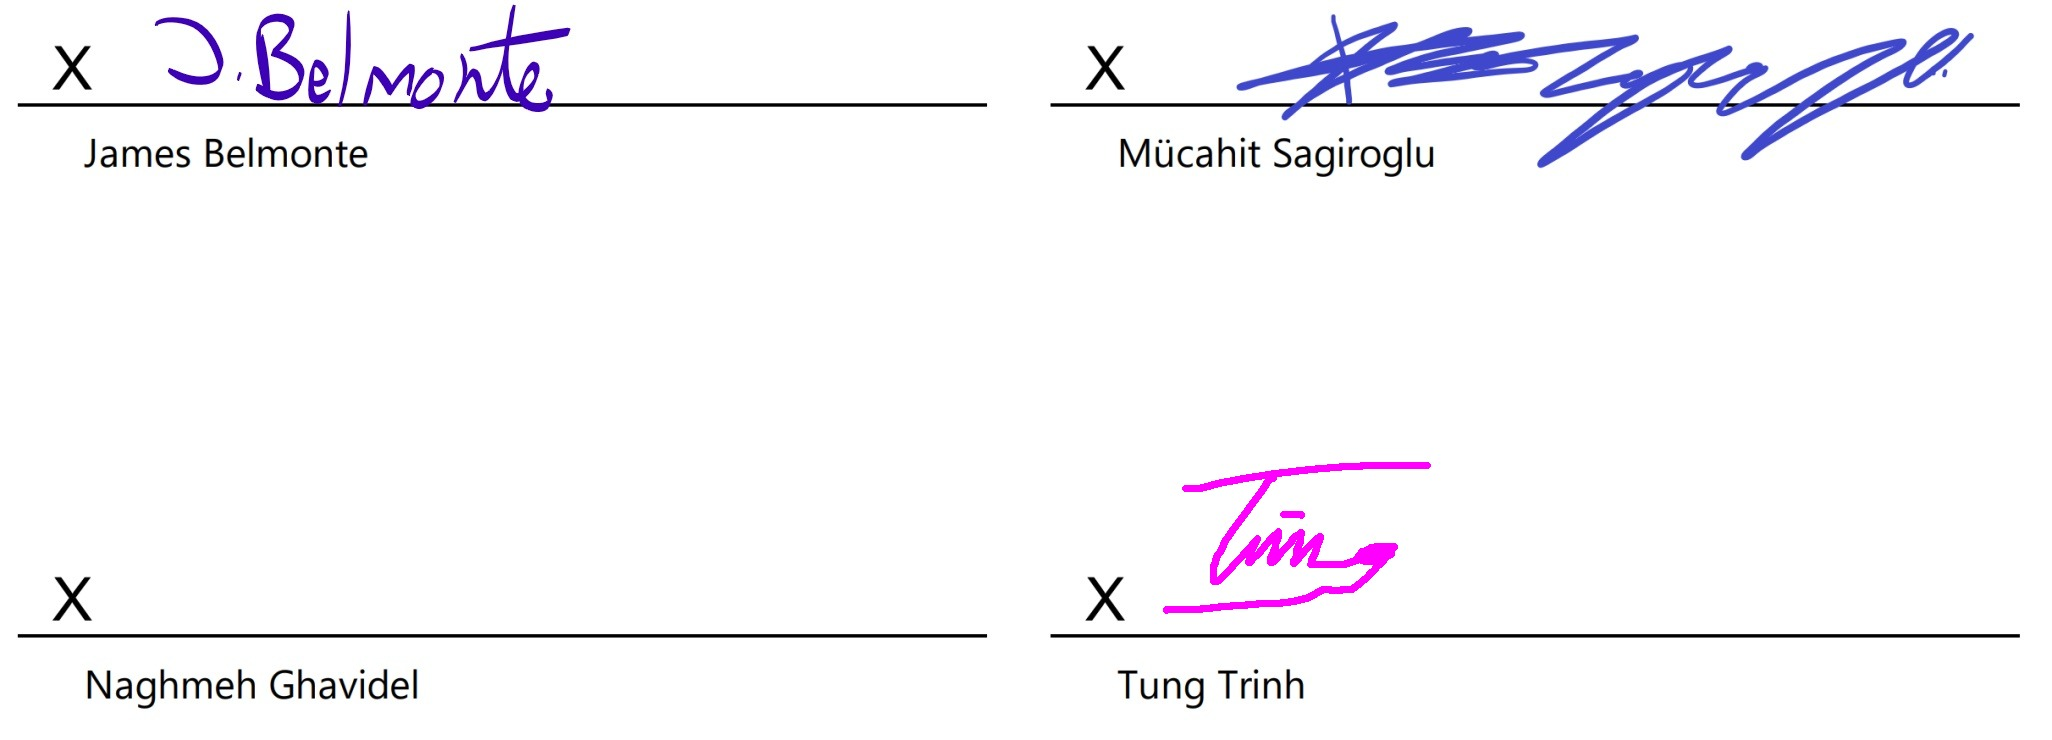
\includegraphics[width=1\linewidth]{Bilder/unterschrift}
\end{figure}

%Inhaltsverzeichnes & Abbildungsverzeichnis & Tabellenverzeichnis
\tableofcontents
\listoffigures
\listoftables
%\lstlistoflistings
%ABKÜRZUNGSVERZECIHNIS
\chapter{Abkürzungsverzeichnis}
\begin{acronym}
	\acro{k}[ADSL]{Asymmetric Digital Subscriber Line}
	\acro{k}[bzw.]{beziehungsweise}
	\acro{k}[CLI]{Command Line Interface}
	\acro{k}[DHCP]{Dynamic Host Configuration Protocol}
	\acro{k}[DNS]{Domain Name System}
	\acro{k}[ESP]{Encapsulating Security Payload}
	\acro{k}[HTTP]{Hypertext Transfer Protocol }
	\acro{k}[HTTPS]{Hypertext Transfer Protocol Secure}
	\acro{k}[ISP]{Internet Service Provider}
	\acro{k}[LAN]{Local Area Network}
	\acro{k}[MTU]{Maximum Transmission Unit}
	\acro{k}[NAT]{Network Address Translation}
	\acro{k}[OF]{OpenFlow}
	\acro{k}[OSI-Modell]{Open Systems Interconnection model}
	\acro{k}[SDN]{Software Defined Network}
	\acro{k}[SDSL]{Symmetric Digital Subscriber Line}
	\acro{k}[usw.]{und so weiter}
	\acro{k}[VPN]{Virtual Private Network}
	\acro{k}[WAN]{Wide Area Network}
\end{acronym}


%Aktivierung arabische Seitenzahlen
\mainmatter % Seite fängt mit 1 an

%Kapitel: Einleitung
\chapter{Abstract}
{\tiny Verfasst von: Name, Name\par}
Der vorliegende Projektbericht dient als Dokumentation des Informatikprojekts „Software-Defined Network mit OpenFlow“ an der Frankfurt University of Applied Sciences im Bachelorstudiengang Informatik im Wintersemester 2021/2022.\par
Das Aufkommen des Internets hat eine Revolution in der Informationstechnologie geschaffen. Durch eine neue Art der Kommunikation kann der Mensch auf nationaler wie auch auf internationaler Ebene effizienter und effektiver Informationen weitervermitteln. Dies bildet die Grundlage für die heutige Wissensökonomie.\par
Die traditionelle Netzwerkarchitektur ist jedoch seit einem halben Jahrhundert unverändert geblieben und wird für die Geschäftsanforderungen von Unternehmen, Netzwerkbetreibern und Endbenutzern zunehmend ungeeignet. Gegenwärtig werden die Geschäftsanforderungen von Unternehmen immer komplexer und die Anwendungsvielfalt der Endbenutzer nimmt zu, was zu unterschiedlichen Anforderungen der Benutzer an Verbindungsnetzwerke führt. Das Netzwerk muss auf sich schnell ändernde Parameter von Latenz, Bandbreite, Routing, Sicherheit und so weiter (usw.) entsprechend den Anforderungen der Anwendungen reagieren \cite{case}.\par
In den letzten Jahren hat die dramatische Zunahme der Netzwerkkomplexität Schwierigkeiten bei der traditionellen Netzwerkadministration mit sich gebracht. Das Konfigurieren von Computernetzwerksystemen unter Verwendung vordefinierter Richtlinien, das Rekonfigurieren von Netzwerken, um auf Änderungen zu reagieren, die Fehlerkorrektur und der Lastausgleich sind zu gewaltigen Aufgaben geworden. Wenn die Parameter des Netzwerks neu konfiguriert wurden, musste jedes Gerät manuell vollständig neu konfiguriert werden, anstatt einfach nur den Teil der Steuerungsebene zu ändern (vgl. Kim/Feamster 2013: 114f). Dies führte zu einem revolutionären Wandel in der Netzwerktechnologie durch die Zentralisierung der Netzwerkadministration. Seitdem wurde das Konzept des Software-Defined Network (SDN) geboren \cite[114-115]{improve}. 


\section{Software-defined Networking}\label{sdn}
Im folgenden Abschnitt werden die jeweiligen Einleitungen jedes Mitgliedes vorgestellt. Sie dienen als separate Einleitungen zum Projektbericht.

\subsection{Einleitung von James}\label{einl-james}
asddsa
\subsection{Einleitung von Naghmeh}\label{einl-naghmeh}
asddsa
\subsection{Einleitung von Tung}\label{einl-tung}
asddsa
\subsection{Einleitung von Mücahit}\label{einl-müco}
asddsa

\section{Motivation}
{\tiny Verfasst von: Name, Name\par}
Das Modul “Informatik Projekt” wird im 5. Semester des Bachelorstudiengangs Informatik durchgeführt. Nach erfolgreichem Abschluss des Moduls sollten Studierende gewisse Kompetenzen erlernt haben, wie beispielsweise den Software-Engineering Prozess planen und durchführen, als auch auf einem vertieften Niveau gemeinsam programmieren zu können. Außerdem sollten Studierende fähig sein, gemeinsam ein Team zu bilden und einen selbsterstellten Zeitplan einzuhalten sowie auf einem technisch hohen Niveau zu kommunizieren, um als Team auf Ergebnisse zu kommen. Falls unerwartete Komplikationen sowohl technischer als auch sozialer Art entstehen, sollte als Team diese Hürde überwunden werden. Infolgedessen entstand dieser Projektbericht, der als Projektergebnis und als Dokumentation dient, um die erlernten Kompetenzen widerzuspiegeln.\par
Durch das Thema “Software-Defined Networking mit Openflow” konnte Freizeit mit Studium verbunden werden, da viele selbsterlernte Kenntnisse und Vorkenntnisse aus anderen Modulen praktisch angewendet werden konnten. Zugleich dient die Dokumentation durch ausführliche Erklärungen und Abbildungen auch als Tutorial, dass den Einstieg in das Thema SDN durch Praxis vereinfachen soll.
\section{Problemstellung}
{\tiny Verfasst von: Name, Name\par}
Innerhalb des Informatikprojekts muss sich folgendes Szenario vorgestellt werden:\par
Ein Unternehmen plane eine Netzwerkkommunikation zwischen vier Standorten mittels Sofware-Defined Networking Funktionen. Die Hauptverwaltung befinde sich in Frankfurt am Main, die drei weiteren Niederlassungen seien in München, Berlin, Hamburg. Zudem sollte jede Lokation einen Asymmetric Digital Subscriber Line Zugang (ADSL) zum Internet haben.\par
Darüber hinaus müssen im Netzwerk bestimmte Funktionen und Aufgaben realisiert werden. Es solle nicht nur für jede Lokation jeweils ein privater IP-Adressenbereich genutzt werden, sondern auch ein Netzwerkplan vom gesamten Netzwerk erstellt werden. Außerdem solle jede Kommunikation zwischen den einzelnen Lokationen über eine Virtual Private Network Verbindung (VPN) laufen, somit sei der gesamte Datenverkehr über das Internet und zwischen den Lokationen verschlüsselt. Anschließend müsse ein Service-Provider gefunden werden, der die gewünschte Konfiguration und Anforderungen realisiere. Jedoch sollen der Preis und die benötigte Bandbreite nicht nur für den Internetzugang, sondern auch für die Wide Area Network-Verbindungen (WAN) beachtet und verglichen werden. Ebenfalls solle durch SDN sowohl eine Network Address Translation-Firewall-Funktion (NAT) als auch eine Webproxy-Funktion in allen Lokationen implementiert werden. Ergänzend dazu solle mithilfe des SDN-Controllers sowohl eine graphische Darstellung der Netzwerkstruktur durch einen Topologieviewer realisiert werden als auch eine Monitoring-Lösung. Zudem müsse eine Quality of Service -Funktion implementiert werden, die genügend Bandbreite für Audio beziehungsweise (bzw.) Video-Konferenzen habe, auch wenn diese über die WAN-Verbindung mit Symmetric Digital Subscriber Line (SDSL) 20 Megabit begrenzt sei. Anschließend wird ein weiteres Szenario beschrieben:\par
“Für eine Spezialanwendung muss eine Software in Berlin wichtige Daten an einem Server in der Zentrale senden, dazu kann diese Software über die API mit dem Controller kommunizieren und diesem dies mitteilen. Dadurch wird der Controller nun alle Knoten auf diesem Weg durchs Netzwerk anweisen, diesen Flow zu priorisieren und alle anderen Datenströme zu drosseln.” 
Schließlich sollen die Netzwerkfunktionen Hub (Repeater), Bridge, Layer-2-Switch, Layer-3-Switch, Dynamic Host Configuration Protocol (DHCP) und Domain Name System (DNS) analysiert und realisiert werden.\par
In Kapitel 3 wird für die Implementierungen der Netzwerk Funktionalitäten Screenshots von Mininet in VirtualBox gezeigt, die als Nachweis der einzelnen Funktionalitäten dienen sollen.


\section{Aufbau der Arbeit}
{\tiny Verfasst von: Name, Name\par}
In Kapitel 2 dieser Projektarbeit wird über das generelle Vorgehen in dem Projekt geschrieben. Nach einer kurzen Vorstellung unseres Projektziels, wird das konkrete Vorgehen innerhalb der Gruppe erläutert. Weiterhin wird sowohl über die Festlegung der Meilensteine, als auch über die genutzten Werkzeuge eingegangen. In Kapitel 3 wird die Projektdurchführung erklärt und in den Unterkapiteln werden die erreichten Ergebnisse vorgestellt, die auch die einzelnen Thematiken der jeweiligen Funktionalitäten ergänzen. Anschließend dient Kapitel 4 mit einer kurzen Analyse aller Ergebnisse, als auch eine kritische Betrachtung der Projektanforderung, als Auswertung und Selbstreflektion, was im Rahmen der Projektarbeit nicht funktionierte und umgesetzt werden konnte, in Bezug auf Netzwerkanforderungen, sowie intern zwischen allen Gruppenmitgliedern. Kapitel 5 bildet mit dem Fazit einen Ausblick in die mögliche Zukunft für SDN.


\chapter{Projekt}
\section{Projektziel}
{\tiny Verfasst von: Name, Name\par}
Ziel des Projekts war es, ein Netzwerk für ein Unternehmen mit vier Lokationen aufzubauen. Dabei war es besonders wichtig, dass das gesamte Netzwerk mit SDN Funktionen realisiert wurde.\par
Ein stabiles Netzwerk vom ersten Tag an wird die Grundlage für den Erfolg von Unternehmen sein. Damit Unternehmen gut funktionieren, muss auch das Netzwerksystem gut funktionieren. Das Netzwerk arbeitet mit der richtigen Kapazität und bringt Effizienz. Die Aufgabe war es, ein gutes stabiles Netzwerk aufzubauen, dass zu 100 Prozent bei Datenverkehr funktionierte und unerwartete Sicherheitsprobleme vermeidete.\par
Das Netzwerksystem musste eng verwaltet und überwacht werden. Zudem musste es leicht unterstützt werden, um Probleme auf die effektivste Weise behandeln und beheben zu können. Es war zwingend erforderlich, dass das Netzwerksystem sicher und verschlüsselt war. Denn Unternehmensdaten sind das Wichtigste. Bei der Netzwerksicherheit ging es auch um den Schutz von Unternehmensressourcen. Je nach Verwendungszweck und Anzahl der Nutzer sollten genügend Bandbreite zur Verfügung gestellt werden.\par
Im Laufe des Projektberichtes werden die erfolgreichen sowie erfolglosen Ergebnisse des Projekts dokumentiert und dargestellt. Am Ende des Projektes wird ein lauffähiges Produkt entstehen, dass alle benötigten Funktionalitäten erfüllt.  

\section{Vorgehen}
{\tiny Verfasst von: Name, Name\par}
Angemessene Aufgabenverteilung im Kollektiv, brachte viele Vorteile für die Arbeitssituation und den Teammitgliedern. Die Nutzung der maximalen Kapazität jedes Teammitglieds war ein effektiver Weg, um die Arbeitseffizienz zu verbessern.\par
Um die Wünsche und Fähigkeiten jedes einzelnen Mitglieds zu verstehen, wurden Gespräche und Diskussionen frühzeitig durchgeführt. Die Zuweisung von Aufgaben, die der Produktivität jeder Person entsprachen, half den Mitgliedern, effektiver und mit einem angenehmeren Geist zu arbeiten. Den Mitgliedern wurden bestimmte Aufgaben mit Fristen zugewiesen. Es wurde jede Woche ein permanentes Treffen über Discord gehalten. Spontane Treffen konnten mit dem höchsten Geist und der höchsten Konzentration ebenfalls durchgeführt werden.\par
Die Analyse von Aufgabenzuweisungen war wichtig, um zu verstehen, was getan werden muss und welche Tools notwendig seien. Der Wissensaustausch half den Mitgliedern, sich Wissen sofort anzueignen und effektiv zu nutzen. Nach einer erfolgreichen Analyse begann unser Team mit der Ausarbeitung eines Plans. Die Arbeit wurde vom Projektleiter aufgeteilt und kontrolliert.

\section{Festlegen von Meilensteinen}
{\tiny Verfasst von: Name, Name\par}
In dem ersten Treffen der Gruppe wurde entschieden, drei zentrale Meilensteine zu definieren (siehe Abbildung \ref{milestones}). Grund dafür sei, einen klaren Faden in der Projektarbeit zu konstruieren, um mit der Menge an Informationen strukturiert umgehen zu können. Die Meilensteine wurden mithilfe der Aufgabenstellungen konkretisiert:

\begin{figure}[H]
 \centering
 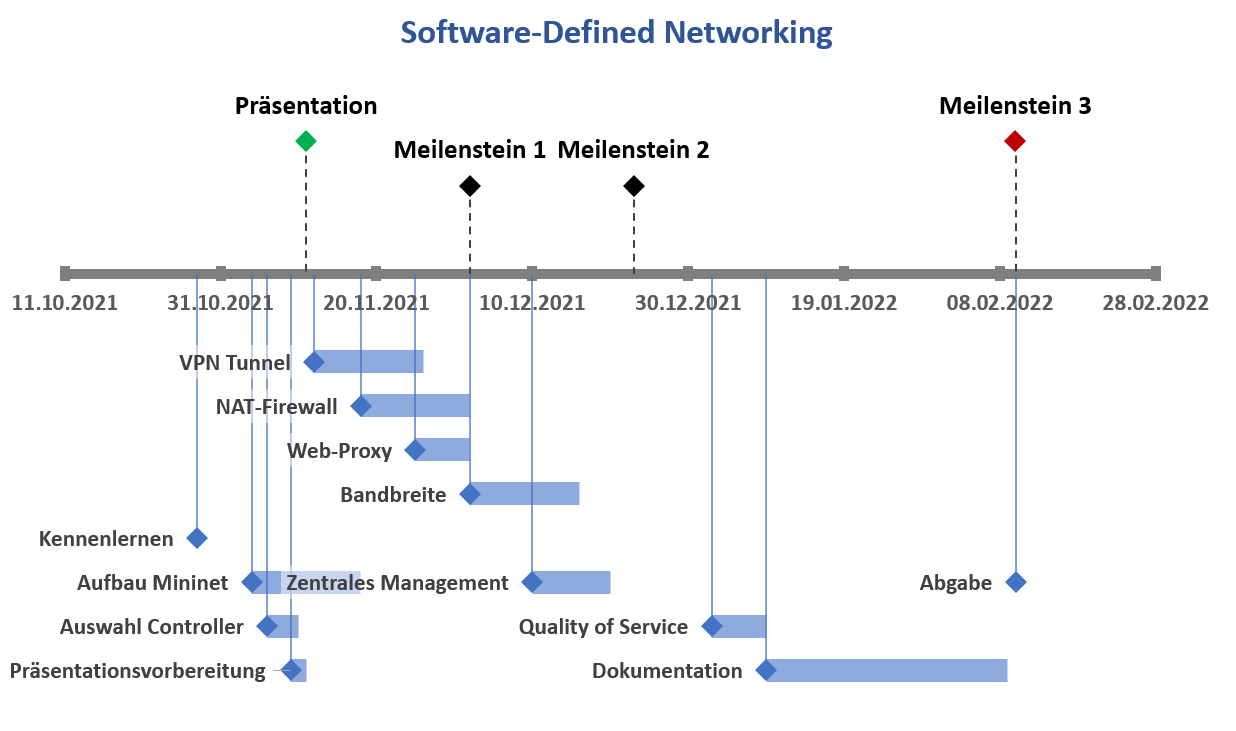
\includegraphics[width=1.0\textwidth]{Bilder/meilensteine}
 \captionsetup{justification=centering,margin=2cm}
 \caption{Zeitplan des Projektes}
 \label{milestones}
\end{figure}

\textbf{Meilenstein 1}
\begin{itemize}
 \item Erstellung eines Netzwerkplans für das gesamte Netzwerk
 \item Kommunikation zwischen Lokationen soll über eine VPN Verbindung realisiert werden
 \item Produktauswahl bei einem ISP zur Realisierung des Netzwerkes
 \item Implementierung einer NAT-Firewall-Funktion in allen Lokationen
 \item Deadline: 02.12.2021
\end{itemize}

\textbf{Meilenstein 2}
\begin{itemize}
 \item Implementierung einer Webproxy-Funktion für den Internet-Zugang in den einzelnen Lokationen
 \item Implementierung eines Topologie-Viewers und einer Monitoring-Lösung
 \item Implementierung einer Quality of Service Funktion für Audio- und Videokonferenzen
 \item Deadline: 23.12.2021
\end{itemize}

\textbf{Meilenstein 3}
\begin{itemize}
 \item Priorisierung von einem Datenflow mithilfe des Controllers
 \item Analyse und Umsetzung der Netzwerkfunktionen von Hub, Bridge, Layer-2-Switch, Layer-3-Switch, DHCP und DNS
 \item Deadline: 10.02.2022
\end{itemize}

Durch gängige IT-Projektmanagementmethoden, wie beispielsweise die Scrum-Methode, konnten frühzeitig Ergebnisse erzielt werden. Infolgedessen gab es am Ende der Projektarbeit mehr Zeit, um über Kleinigkeiten zu reflektieren.

\section{Verwendete Werkzeuge}
{\tiny Verfasst von: Name, Name\par}
Im Folgenden werden die für die Implementierung und Evaluierung verwendeten Hardware- und Softwareumgebungen kurz beschrieben.\par
Dieses Projekt wurde auf VirtualBox Oracle VM Version 6.1 durchgeführt. Unter der Verwaltung von VirtualBox wurde Mininet-Emulator Version 2.3 und Floodlight Controller Version 1.2 installiert. Zur Ausführung von Programmen zur Evaluation wurde außerdem Python3 installiert. Weitere Programme sind auch installiert und sie werden im Ablauf von Kapitel 3 bekannt gegeben und ausführlicher erklärt.

\subsection{Mininet}
{\tiny Verfasst von: Tung\par}
Der Mininet-Emulator implementiert die Verbindung zwischen Switches und Controllern. Diese ermöglicht es Entwicklern, die an der Erstellung und dem Testen von Controller-Ressourcen interessiert sind, Mininet zur Durchführung ihrer Simulationen zu nutzen \cite{mininetoverview}.

\subsubsection{Einführung}
{\tiny Verfasst von: Tung\par}
Mininet ist ein Netzwerk Emulator, mit der Netzwerke simuliert werden können. Bei Mininet handelt es sich um eine kostenlose Open-Source-Software, die die virtuelle Maschine und dem Controller die Recherche in SDN und OpenFlow ermöglicht. Mininet ermöglicht eine sehr groß angelegte Topologie, wodurch ein Netzwerk von Hosts, Switches, virtuellen Links und einem Controller erstellt wird \cite[139]{mininetdefinition}. Das Ausführen von Tests mit den Komponenten ist unkompliziert und kann über Python-Schnittstelle erledigt werden. Benutzer können ihre eigene Netzwerktopologie-Struktur nach ihren eigenen Bedürfnissen aufbauen\cite[141]{mininetdefinition}.

\subsubsection{Funktionalität}
{\tiny Verfasst von: Tung\par}
Mininet:
\begin{itemize}
 \item stellt ein einfaches Netzwerk Testbed dar, welches aber auch gleichzeitig günstig ist. Da der OpenFlow Switch in Mininet alle Eigenschaften wie ein echter OpenFlow Switch hat, ist die Anwendung von einem Netzwerkemulator mit Mininet praktisch sinnvoll.
 \item ermöglicht das Debuggen und Ausführen von Tests größerer Netzwerke mithilfe von Command Line Interface (CLI).
 \item unterstützt das Einrichten beliebiger benutzerdefinierter Diagramme. Die Anwendungen im Mininet können im echten Netzwerk realisiert werden, ohne dass der Code geändert werden muss.
 \item bietet eine benutzerfreundliche und erweiterbare Python-API.
 \item ermöglicht mehreren gleichzeitigen Entwicklern, unabhängig voneinander an derselben Topologie zu arbeiten.
 \item ermöglicht komplexe Topologietests, ohne dass ein physisches Netzwerk verkabelt werden muss \cite{mininetoverview}.
\end{itemize}

\subsubsection{Nachteile}
{\tiny Verfasst von: Tung\par}
Aktuell ist Mininet nur unter Linux lauffähig. Nutzer eines anderen Betriebssystems müssen auf Linux entweder durch Simulierung oder Installation zurückgreifen. Zudem könnte der Sourcecode effizienter und sauberer implementiert werden.\par
Mininet schreibt Ihren OpenFlow-Controller nicht für Benutzer. Wenn Benutzer benutzerdefiniertes Routing- oder Schaltverhalten benötigen, müssen Benutzer einen Controller mit den erforderlichen Funktionen finden oder entwickeln.\par
Standardmäßig ist Mininet-Netzwerk von Local Area Network (LAN) und vom Internet isoliert - das ist normalerweise eine gute Sache! Benutzer können jedoch das NAT-Objekt und/oder die Option --nat verwenden, um Ihr Mininet-Netzwerk über Network Address Translation mit Ihrem LAN zu verbinden. Benutzer können Ihrem Mininet-Netzwerk auch eine echte (oder virtuelle) Hardware-Schnittstelle hinzufügen (siehe Beispiele/hwintf.py für Details).\par
Standardmäßig teilen sich alle Mininet-Hosts das Host-Dateisystem und den PID\hyp{}Speicherplatz. Das bedeutet, dass Benutzer möglicherweise vorsichtig sein müssen, wenn sie Daemons ausführen, die eine Konfiguration in /etc erfordern, und Benutzer müssen darauf achten, dass sie nicht versehentlich die falschen Prozesse beenden. \par
Im Gegensatz zu einem Simulator hat Mininet keine starke Vorstellung von virtueller Zeit. dies bedeutet, dass Timing-Messungen auf Echtzeit basieren und dass Ergebnisse schneller als Echtzeit (z. B. 100-Gbit/s-Netzwerke) nicht einfach emuliert werden können \cite{mnnachteile}.

\subsubsection{Komponenten}
{\tiny Verfasst von: Tung, Naghmeh, James, Mücahit\par}
Ein Mininet-Netzwerk besteht aus den folgenden Komponenten:
\begin{itemize}
 \item \textbf{Link:} Links sind virtuelle Ethernets, die zwei virtuelle Schnittstellen verbinden. Jeder Link verhält sich für das gesamte System wie ein echter funktionsfähiger Ethernet-Anschluss. Die Datenrate jedes Links wird von Linux Traffic Control (TC) festgelegt.
 \item \textbf{Hosts:} Ein emulierter Host ist eine Reihe von Prozessen auf Benutzerebene, die in einen Netzwerk-Namespace verlagert wird. Netzwerk-Namespaces bieten Prozessgruppen privaten Besitz von Schnittstellen, Ports und Routing-Tabellen.
 \item \textbf{Switch:} Mininet verwendet Open vSwitches, die im Kernelmodus ausgeführt werden, um Pakete zwischen verschiedenen virtuellen Netzwerkschnittstellen auszutauschen. Open vSwitches sind OpenFlow-fähig und bieten die gleiche Semantik für das Senden von Paketen wie einen realen Switch.
 \item \textbf{Controller:} Ein Controller ist in der Mininet-Simulation ein Knoten, der einen OpenFlow-Controller darstellt. Mininet bietet die Möglichkeit einen internen oder externer Controller zu benutzten. Für den externen Controller wird die IPv4-Adresse und der Port benötigt.
\end{itemize}


\subsubsection{Installation}
{\tiny Verfasst von: Tung\par}
Mininet kann auf verschiedene Weisen installiert werden. In unserer Arbeit wurde die Option: Native Installation from Source ausgewählt. Die Installation wird Schritt für Schritt aufgeführt \cite{mnapi}:
\begin{itemize}
\item[1.] Git wird über das Linux-Terminal installiert
\end{itemize}
\colorbox{CadetBlue}{\textcolor{white}{\textbf{\textsf{\$ sudo apt-get install git}}}}
\begin{itemize}
\item[2.] Über das git Kommando wird die aktuellste Version von Mininet installiert
\end{itemize}
\colorbox{CadetBlue}{\textcolor{white}{\textbf{\textsf{\$ git clone git://github.com/mininet/mininet}}}}
\begin{itemize}
\item[3.] Mit install.sh die Installation starten
\end{itemize}
\colorbox{CadetBlue}{\textcolor{white}{\textbf{\textsf{\$ sudo mininet/util/install.sh -a}}}}

\subsubsection{Aufbau}
{\tiny Verfasst von: Tung\par}
Durch die Eingabe von dem Befehl \textit{\textbf{sudo mn}} wird ein Standardnetzwerk mit zwei Hosts, einer Switch und einem Controller gestartet (siehe Abbildung \ref{sudomn}).

\begin{figure}[H]
 \centering
 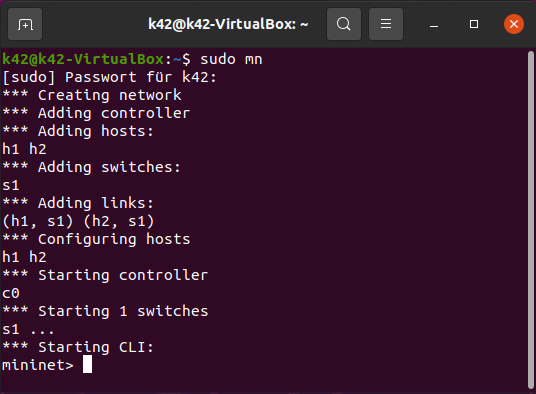
\includegraphics[width=0.5\textwidth]{Bilder/sudomn}
 \captionsetup{justification=centering,margin=2cm}
 \caption{Erstellung eines Standardnetzwerkes mit Mininet}
 \label{sudomn}
\end{figure}

\subsection{Floodlight}
{\tiny Verfasst von: Mücahit, Tung\par}
Floodlight ist ein sogenannter SDN-Controller in der Control Plane. Dieser kommuniziert mit der Data Plane über ein Kommunikationsprotokoll namens OpenFlow und verwaltet diesen \cite[161]{floodlightdefinition}.

\subsubsection{Einführung}
{\tiny Verfasst von: Mücahit, Tung\par}
In den letzten Jahren wurde eine Vielzahl unterschiedlicher SDN-Controller entwickelt. Aus diesem Grund gibt es mittlerweile eine riesige Auswahl an SDN-Controllern für die breit gefächerten Einsatzzwecke, wo unteranderem OpenDaylight, Ryu, POX, NOX und Floodlight dazugehören. Mit allen Controllern sollten alle Projektziele der Projektarbeit erreichbar sein \cite{controllers}.\par
{\tiny Verfasst von: Mücahit\par}
Floodlight wurde als Controller ausgewählt, da einige Punkte und das daraus resultierende Gesamtprodukt die Gruppe überzeugen konnte. Dazu gehört unteranderem die einfache und gut beschriebene Installation. Die moderne Webbenutzeroberfläche und die verständliche, gut dokumentierte REST-API sind sehr benutzerfreundlich und leicht zu verstehen. Daraus resultiert auch die Option, die REST-API über ein Python-Skript zu benutzen. Die Einbindung des Floodlight-Controllers in Eclipse ermöglicht die Implementierung, Untersuchung und das Debuggen verschiedenster Controller-Funktionen. Die gute Dokumentation des in Java geschriebenen Controllers und einige mit der Installation mitgelieferten Module geben dem Entwickler einen guten Start zur Entwicklung von Netzwerkfunktionen.

\subsubsection{Funktionalität}
{\tiny Verfasst von: Mücahit\par}
Die Funktionalitäten des Floodlight-Controllers unterscheiden sich anhand der Ausführung und der Implementierung. Funktionen können über die Webbenutzeroberfläche per Eingabe ausgeführt werden (siehe Abbildung \ref{webui}). Das Einstellen der Firewall und der Access Control List sind zwei dieser Funktionen. Nach Aktivierung der Firewall werden alle Pakete, die nicht in der Liste eingetragen sind, fallen gelassen. Die Access Control List arbeitet ähnlich wie die Firewall, wohingegen nur eine Liste mit erwünschten und nicht erwünschten Quellen existiert. Die Quellen werden anhand der Paket-Informationen angegeben. Bei einem Treffer wird die Quelle je nach Einstellung zugelassen oder verweigert. Folglich verweigert die Firewall jegliche Verbindung nach Aktivierung, wohingegen die Access Control List nur bestimmte Zugriffe auf ein Netzwerk zulässt oder ablehnt \cite{firewall}. \par
Auf der Webbenutzeroberfläche sind Informationen zu dem vom Controller gesteuerten Netzwerk einsehbar. Dazu gehört die Anzahl der Switches, Hosts und Links sowie der verbrauchten Ressourcen des Controllers und der Netzwerktopologie. Die Statistikfunktion des Controllers kann auf der Benutzeroberfläche aktiviert werden. Dieser dient zur ausführlichen Weiterverarbeitung und der Anzeige der vom Controller gesammelten Statistik. Dazu gehören die Flow, meter, queue, aggregate, table und port Statistiken. Die Sammlung benutzerdefinierter Statistiken sind ebenfalls möglich und müssen vom Entwickler nachimplementiert werden. Über die REST-API können sogenannte Flows eingetragen werden, die zur Steuerung des Netzwerkes beitragen. Dabei können Datenpakete modifiziert, zwischengespeichert und umgeleitet werden \cite{statistik}.

\begin{figure}[H]
 \centering
 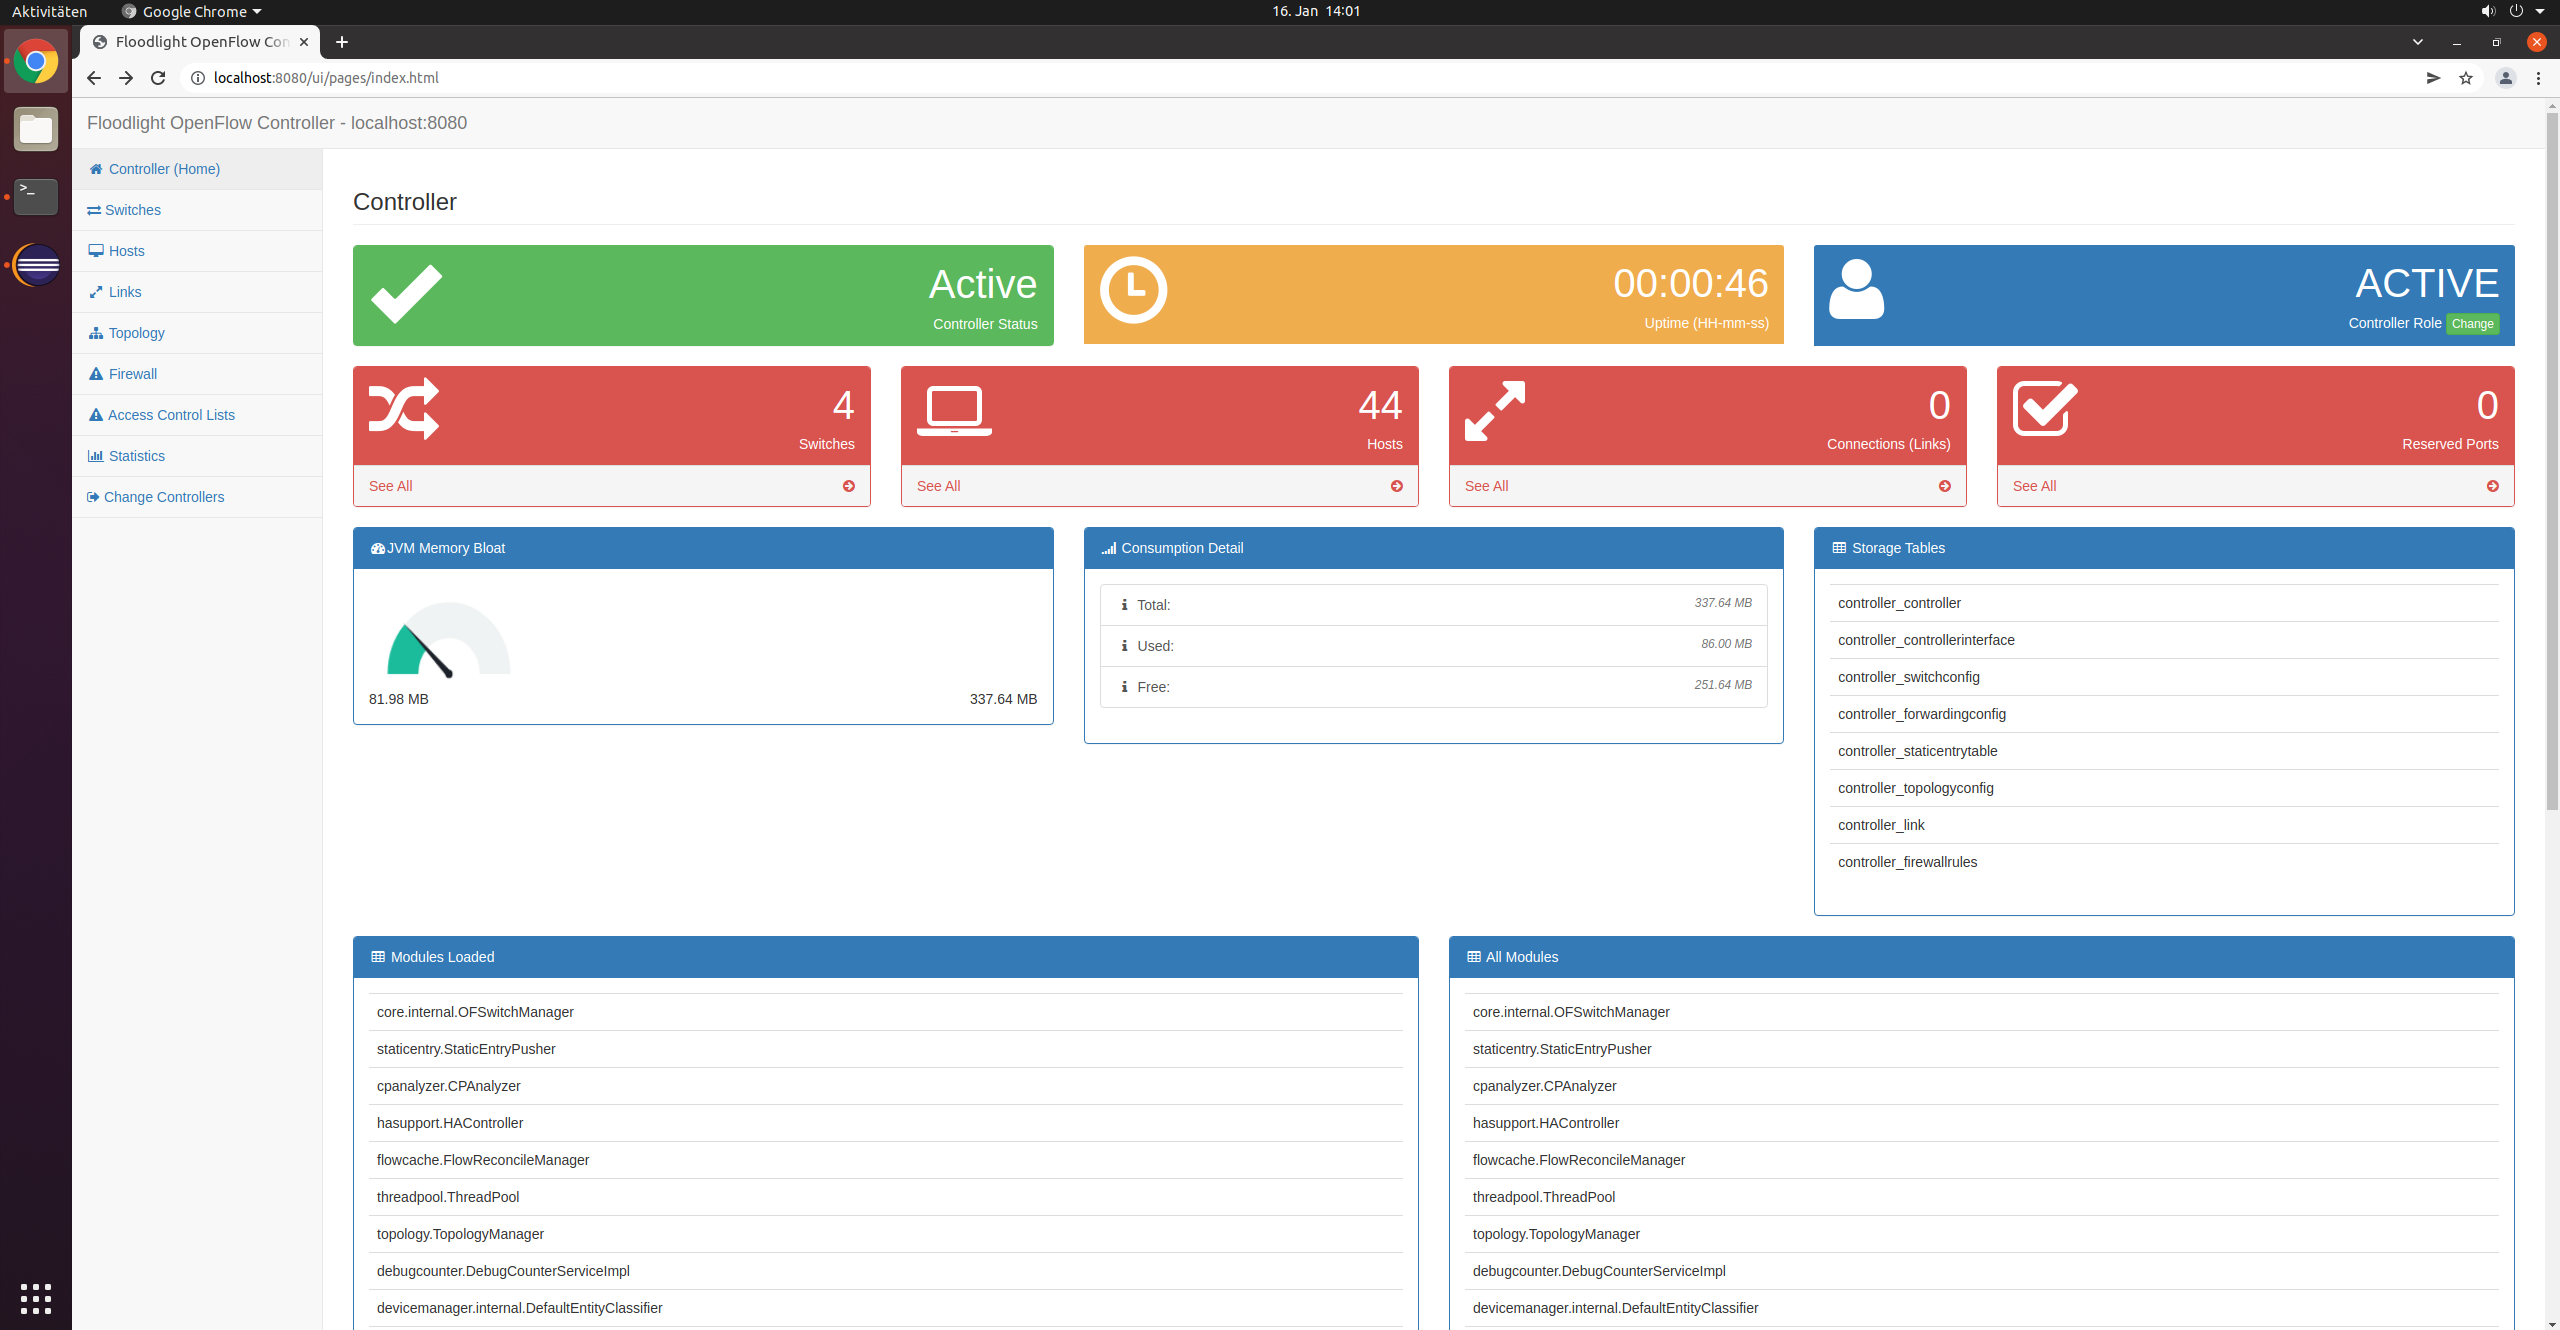
\includegraphics[width=1.0\textwidth]{Bilder/webui}
 \captionsetup{justification=centering}
 \caption{Webbenutzeroberfläche vom Floodlight-Controller}
 \label{webui}
\end{figure}


\subsubsection{Nachteil}
{\tiny Verfasst von: Mücahit\par}
Das ganze Netzwerk ist betroffen, wenn Floodlight ausfällt oder nicht erreichbar ist. Dieser Single Point of Failure gilt für alle Controller und stellt ein Risiko für Netzwerke, die eine hohe Verfügbarkeit und Zuverlässigkeit fordern\cite{failure}. Die Wartung und Konfiguration eines Controllers für komplexe Netzwerkstrukturen erfordern viele geschulte Angestellte \cite{floodlightnachteil}.

\subsubsection{Komponenten}
{\tiny Verfasst von: Mücahit\par}
Mit der Installation von Floodlight kommen sogenannte Module zum Einsatz. Die meisten der Module sind bereits aktiviert und stellen bestimmte Funktionen zur Verfügung. Einer davon ist die Learning Switch, welcher für die Speicherung der Routen zu den Hosts zuständig ist. Wenn ein Host einen anderen Host im gleichen Netzwerk erreichen will und der Switch die Route nicht kennt, wird ein Broadcast ausgeführt, der die Anfrage auf allen Ports ausgibt. Wenn der Host antwortet, speichert der Switch die MAC-Adresse des jeweiligen Hosts ab und muss somit keinen Broadcast durchführen \cite{broadcast}. Weitere Beispielmodule wären der Load Balancer, der für einen Ausgleich des Datenverkehrs im gesamten Netzwerk sorgt \cite{loadbalance}. Über die REST-API stellt Floodlight die Netzwerktopologie über die Webbenutzeroberfläche grafisch dar. Es existieren noch weitere Module, wobei auch eigene programmiert werden können \cite{restapi}.

\subsubsection{Installation}
{\tiny Verfasst von: Mücahit\par}
Die Installation des Floodlight-Controllers kann auf den Betriebssystemen Linux, Mac oder Windows erfolgen. Es wird das Java Development Kit 8, Maven, Git, build-essential und das Python Development Paket benötigt. Da Floodlight in Java geschrieben wurde, wird auch zur Ausführung Java verwendet. Maven wird zum sogenannten Builden benutzt, bei dem die Software Floodlight aus mehreren Dateien zusammengestellt wird. Das Python Development Paket wird zur Ausführung und Git zum Herunterladen von Floodlight vorausgesetzt. Build-essential werden zum Kompilieren einiger Software verwendet. Im Folgenden wird die Installation auf Linux Schritt für Schritt erklärt. Befehle müssen im Linux-Terminal zeilenweise eingegeben werden.

\begin{itemize}
\item[1.] Alle benötigten Abhängigkeiten installieren.
\end{itemize}
\colorbox{CadetBlue}{\textcolor{white}{\textbf{\textsf{\$ sudo apt-get install build-essential git maven python-dev openjdk-8-jdk}}}}
\begin{itemize}
\item[2.] Java Compiler als Alternative festlegen. Befehl eingeben und JDK 8 Auswählen.
\end{itemize}
\colorbox{CadetBlue}{\textcolor{white}{\textbf{\textsf{\$ sudo update-alternatives --config javac}}}}
\begin{itemize}
\item[3.] Programmcode per Github herunterladen und aktualisieren
\end{itemize}
\colorbox{CadetBlue}{\textcolor{white}{\textbf{\textsf{\$ git clone git://github.com/floodlight/}}}}\\
\colorbox{CadetBlue}{\textcolor{white}{\textbf{\textsf{\$ floodlight.git}}}}\\
\colorbox{CadetBlue}{\textcolor{white}{\textbf{\textsf{\$ cd floodlight}}}}\\
\colorbox{CadetBlue}{\textcolor{white}{\textbf{\textsf{\$ git submodule init}}}}\\
\colorbox{CadetBlue}{\textcolor{white}{\textbf{\textsf{\$ git submodule update}}}}
\begin{itemize}
\item[4.] Floodlight Ordnerrechte zuweisen und Builden
\end{itemize}
\colorbox{CadetBlue}{\textcolor{white}{\textbf{\textsf{\$ cd ..}}}}\\
\colorbox{CadetBlue}{\textcolor{white}{\textbf{\textsf{\$ sudo chown -hR Benutzername:Gruppenname floodlight/}}}}\\
\colorbox{CadetBlue}{\textcolor{white}{\textbf{\textsf{\$ cd floodlight/}}}}\\
\colorbox{CadetBlue}{\textcolor{white}{\textbf{\textsf{\$ mvn package -DskipTests}}}}
\begin{itemize}
\item[5.] Floodlight im Terminal ausführen (siehe Abbildung \ref{floodlight})
\end{itemize}
\colorbox{CadetBlue}{\textcolor{white}{\textbf{\textsf{\$ java -jar target/floodlight.jar}}}}\par
{\tiny Verfasst von: James\par}
Es besteht die Möglichkeit, den Floodlight Controller mithilfe von Eclipse zu starten, somit muss Floodlight nicht im Terminal ausgeführt werden. Außerdem ist Floodlight durch die Entwicklungsumgebung Eclipse leichterer auszuführen und eine Bearbeitung ist übersichtlicher. Zudem hat man eine schnelle Übersicht vom kompletten Conroller, da alle Klassen in einem Eclipse Ordner einzusehen sind. Mit sudo mvn package –Declipse werden mehrere Dateien erstellt. Mit den neu erstellten Dateien kann ein neues Eclipse Projekt importiert werden. Anschließend wird Eclipse gestartet und eine neue Arbeitsumgebung erstellt. \textit{\textbf{File -> import -> General -> Existing Projects into Workspace}} und auf \textit{\textbf{Next}} klicken. Von \textit{\textbf{Select root directory}} auf \textit{\textbf{Browser}} klicken und Verzeichnis das Floodlight enthält auswählen. Das Projekt mit \textit{\textbf{finish}} ausführen und damit sollte Floodlight auf Eclipse importiert sein.\par
Um Floodlight auf Eclipse auszuführen, wählt man \textit{\textbf{run configuration}} aus, rechts klickt auf \textit{\textbf{java application}} und \textit{\textbf{new}}. Anschließend wird die neue Java Application \textit{\textbf{FloodlightLaunch}} genannt, es nutzt das Projekt Floodlight und \textit{\textbf{net.floodlight.controller-\\.core.Main}} in der Main-Klasse. Nachdem dies konfiguriert wurde, kann das Programm in Eclipse ausgeführt werden.


\subsubsection{Aufbau}
{\tiny Verfasst von: Mücahit\par}
Nach erfolgreicher Installation und Ausführung von Floodlight läuft der Controller standardmäßig auf Port 6653. Im Terminal werden alle informativen Ereignisse ausgegeben. Um den Controller zu stoppen, wird die Tastenkombination Steuerung und C gleichzeitig gedrückt (siehe Abbildung \ref{floodlight}).

\begin{figure}[H]
 \centering
 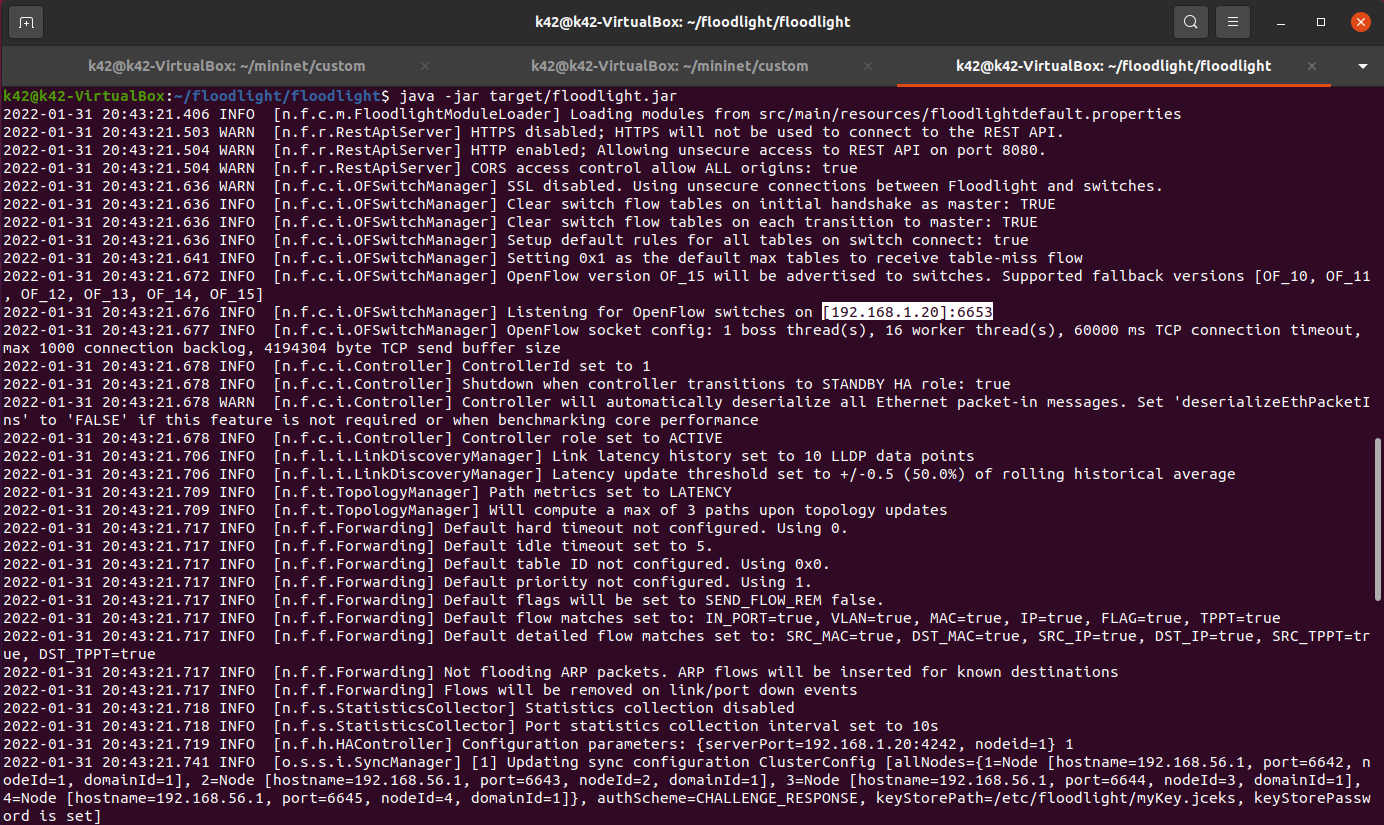
\includegraphics[width=1.0\textwidth]{Bilder/floodlight}
 \captionsetup{justification=centering,margin=1cm}
 \caption{Ausführung von Floodlight über den Linux-Terminal}
 \label{floodlight}
\end{figure}

\newpage
\subsection{Ergebnis}
{\tiny Verfasst von: Tung\par}
%\setlength{\intextsep}{0pt}
%\setlength{\columnsep}{15pt}
\begin{wrapfigure}{R}{0.5\textwidth}
	\vspace{-\baselineskip}
    \centering
    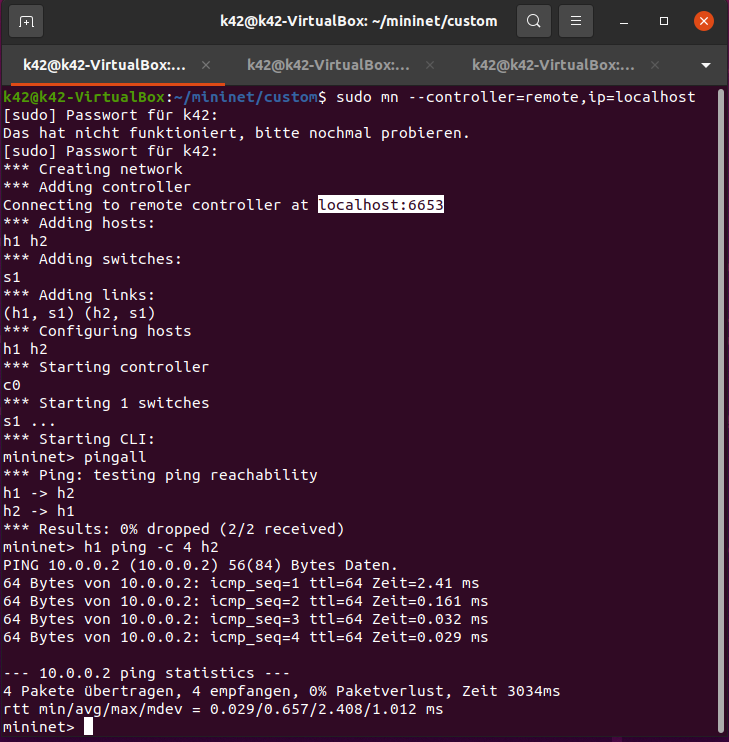
\includegraphics[width=0.5\textwidth]{Bilder/ping}
    \caption{Mininet Controller Verbindung und Ping-Test}
    \label{ping}
\end{wrapfigure}

Nach der Ausführung von Floodlight, wurde dieser mit einer OpenFlow-fähigen Switch verbunden. Der Switch wurde mit Mininet mit der Angabe des Controllers simuliert. Die Konsole zeigt die erfolgreiche Verbindung mit dem Controller. Die Konnektivität im Netzwerk kann mit dem Befehl \textit{\textbf{pingall}} überprüft werden. Die Konnektivität zwischen Host 1 und Host 2 wird durch den Befehl \textit{\textbf{h1 ping h2}} getestet. Durch Wireshark kann der ausgelöste Datenverkehr betrachtet werden (siehe Abbildung \ref{ping}).



\chapter{Durchführung des Projektes}
{\tiny Verfasst von: James?\par}
Die in Kapitel 1.3 dargestellten Problemstellungen werden in diesem Kapitel behandelt und realisiert. Mit den im vorherigen Kapitel erläuterten Werkzeugen wird dieses Projekt umgesetzt. Durch Abbildungen, Code Ausschnitte und Erläuterungen soll die Dokumentation die Vorgehensweise und Überlegungen der Gruppe wiedergeben. 



\section{Netzwerkplan}
{\tiny Verfasst von: Tung, Naghmeh, James, Mücahit\par}
Die topologische Struktur des Netzwerks, die in Mininet erstellt wird, ist in Abbildung \ref{netzwerkplan} dargestellt. Das Netzwerkdiagramm enthält 40 Hosts, 4 Switches, 4 Router und einen Controller. Der Floodlight-Controller hat einen globalen Überblick über die physikalische Topologie. Die 4 Switches sind mit dem Controller verbunden. Zehn Hosts in den jeweiligen Lokationen sind mit einem Switch verbunden. Um die Hosts in jeder Lokation mit dem Internet und mit anderen Lokationen zu verbinden, wird ein Router benötigt. Durch die grüne Linie und den Tunnel wird gezeigt, dass die Kommunikation zwischen Lokationen verschlüsselt sind. Ebenfalls sind alle Router der Lokationen mit dem Internet verbunden, welches durch eine Cloud visualisiert wird.

\begin{figure}[H]
 \centering
 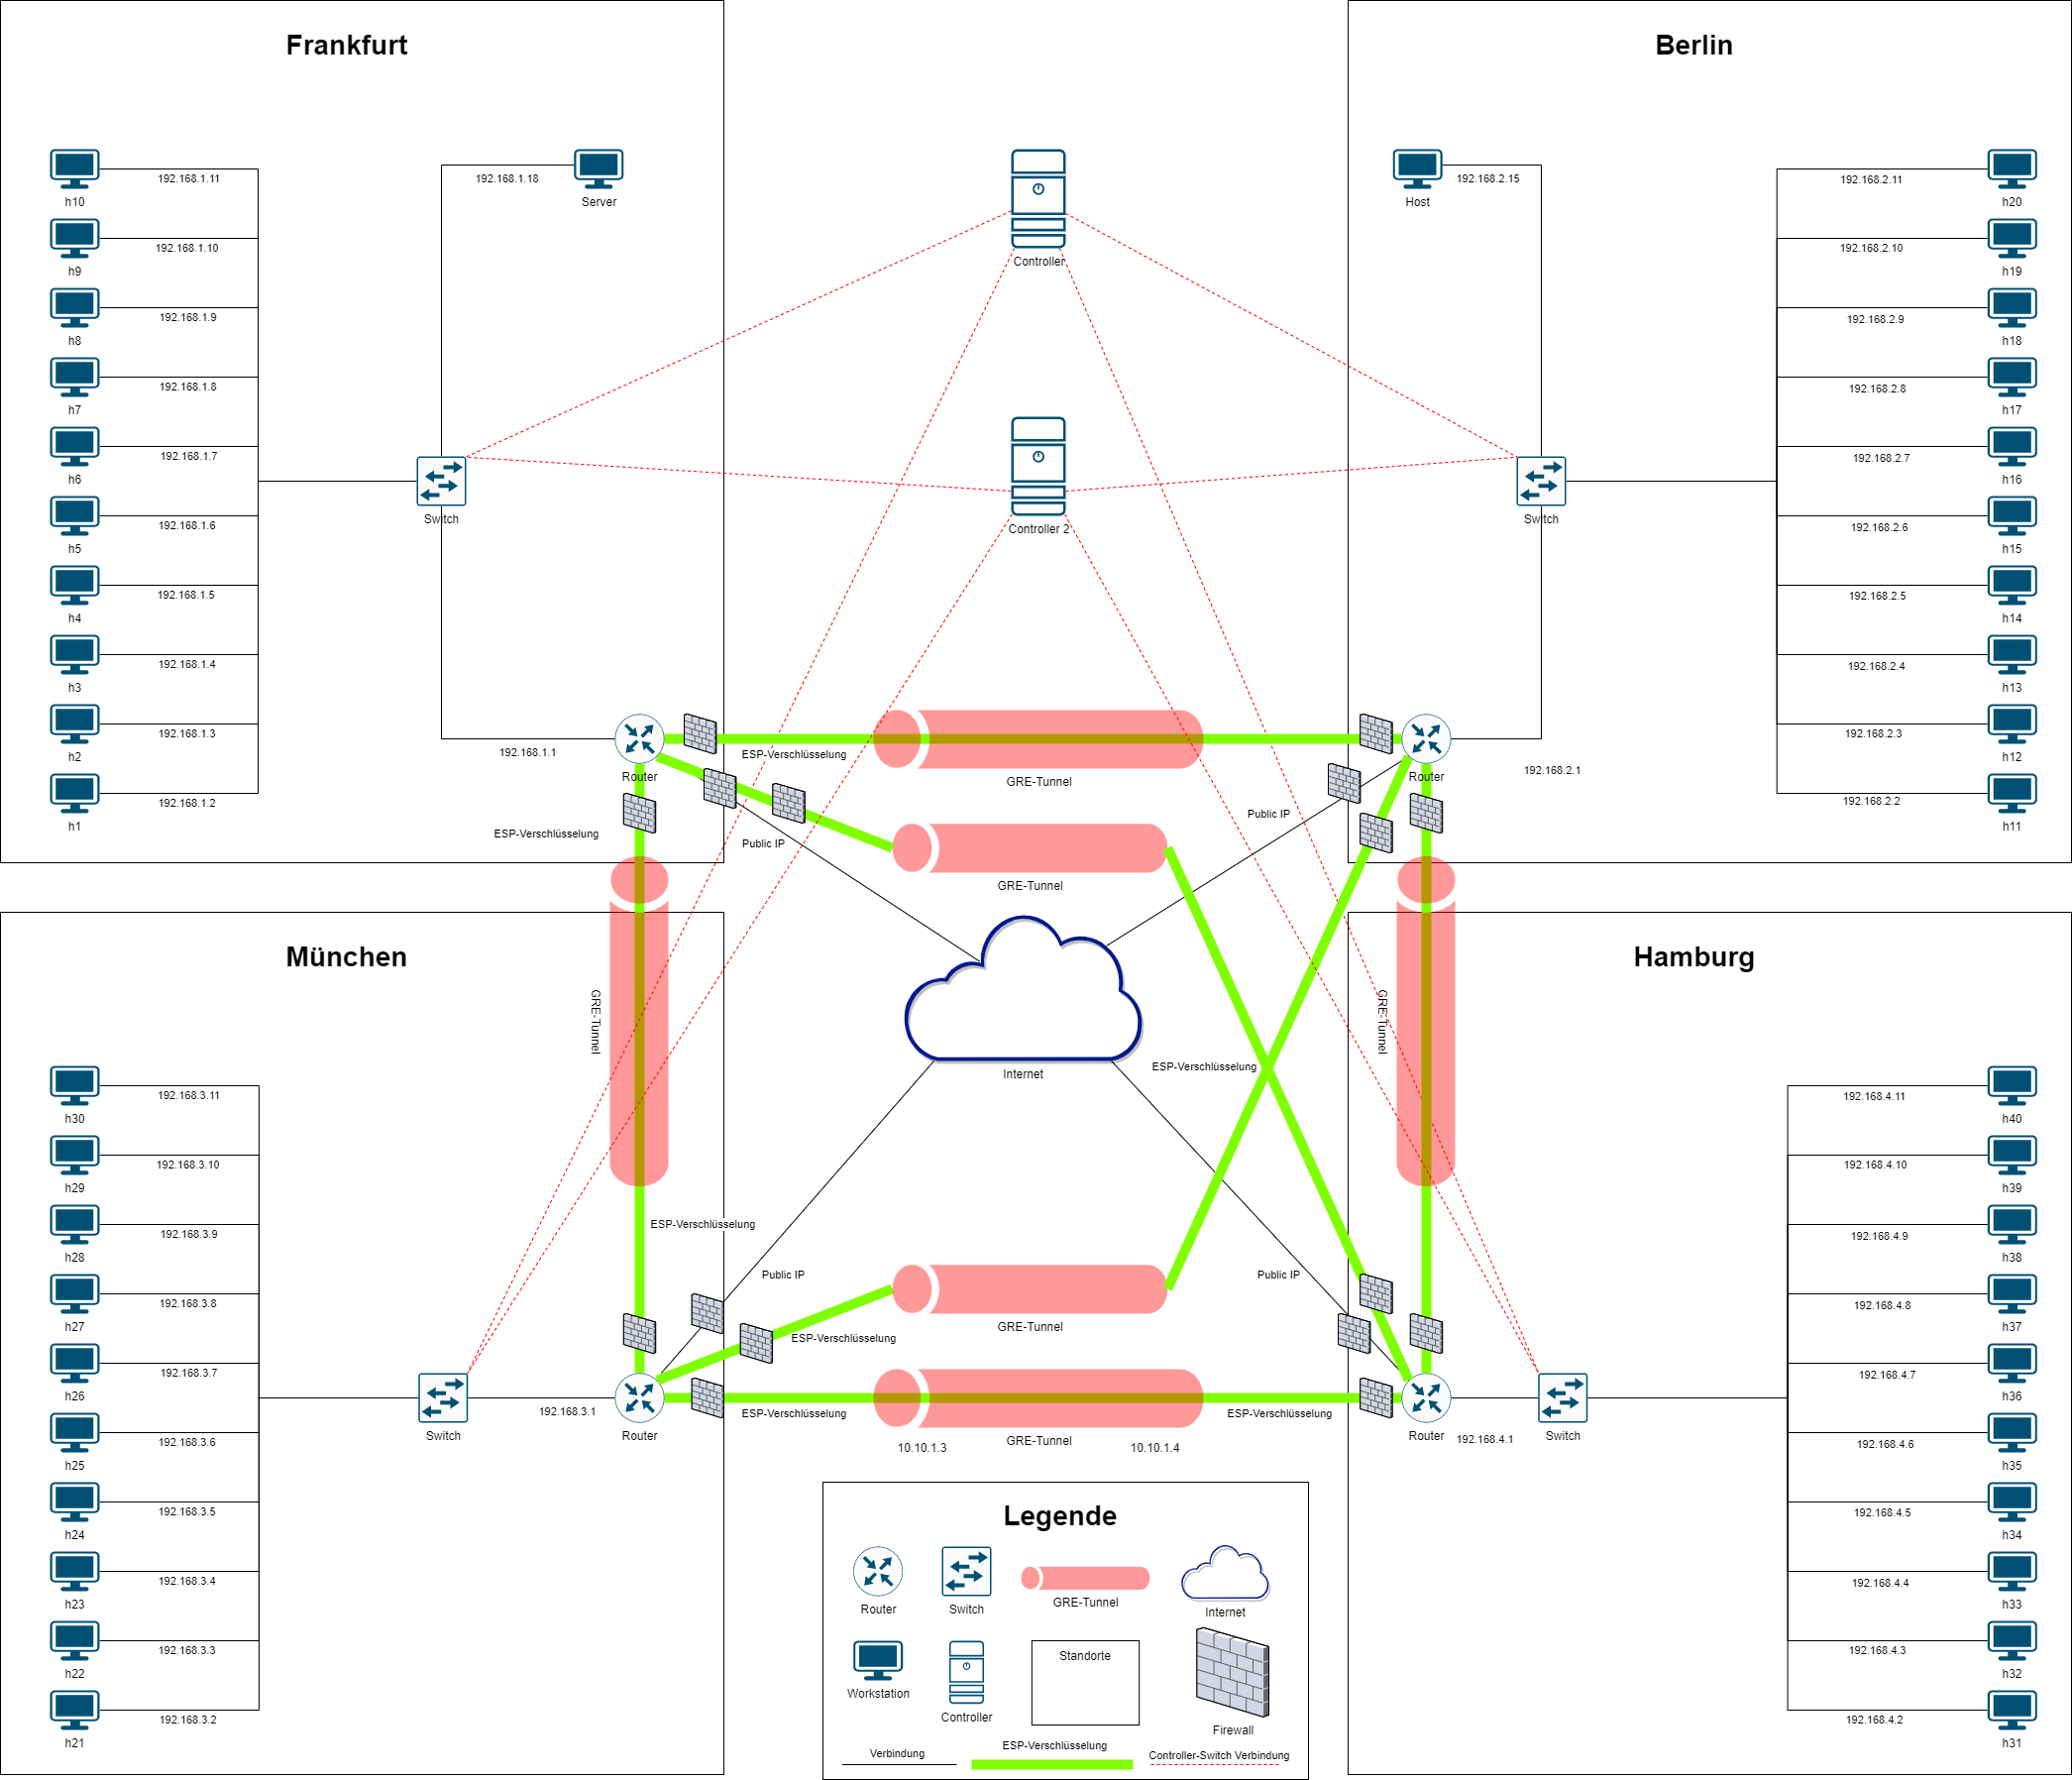
\includegraphics[width=1.0\textwidth]{Bilder/netzwerkplan}
 \captionsetup{justification=centering,margin=1cm}
 \caption{Netzwerkplan aller Lokationen}
 \label{netzwerkplan}
\end{figure}

\begin{table}[H]
	\caption{Vergabe von IPv4-Adressen im Netzwerk}
	\label{netzwerkplan}
	\centering
	\hspace*{-1cm}
	\begin{tabular}{p{3.5cm} p{3cm} p{3cm} p{3cm} p{3cm}}
		\toprule
		 Standort & Frankfurt & Berlin  & München & Hamburg \\
		\midrule 
		Subnetz & 192.168.1.0/24 &  192.168.2.0/24 & 192.168.3.0/24 & 192.168.4.0/24\\
		
		Netzwerkmaske	&255.255.255.0& 255.255.255.0& 255.255.255.0	& 255.255.255.0 \\
		
		Broadcast & 192.168.1.255 &	192.168.2.255 &	192.168.3.255 & 192.168.4.255\\
		
		Router & 192.168.1.1&192.168.2.1& 192.168.3.1 &192.168.4.1\\
		
		Switch & 192.168.1.20& 192.168.2.20&192.168.3.20&	192.168.4.20\\
		
		erster Host& 192.168.1.2& 192.168.2.2& 192.168.3.2&192.168.4.2\\
		
		letzter Host& 192.168.1.254 & 192.168.2.254 & 192.168.3.254 & 192.168.4.254\\
		
	\end{tabular}
	
\end{table}

\section{Aufbau des Netzwerkgerüstes in Mininet}
In diesem Abschnitt wird die beschriebene Topologie unter Verwendung von Mininet simuliert und erklärt.

\subsection{Durchführung}
{\tiny Verfasst von: Tung?\par}
In der Main-Funktion werden die Komponenten eines Netzwerks deklariert und aufgerufen. Das sind eine Topologie, ein Controller mit zugewiesenem Port und ein Mininet Objekt mit der deklarierten Topologie. Anschließend wurde für unsere Router Routing-Regeln und Informationen gegeben.

\subsection{Aufbau der Topologie}
{\tiny Verfasst von: Tung, Mücahit\par}
Die Klasse Netzwerk bildet die Netzwerktopologie. Diese befindet sich in der Main-Funktion des Mininet-Skripts. Das Mininet-Skript besteht aus einer Main-Funktion. Die Main-Funktion enthält eine definierte Klasse \textit{\textbf{Netzwerk()}}. Mithilfe dieser Klasse wird das Netzwerk beziehungsweise eine Topologie erstellt (siehe Abbildung \ref{mininet1}). Die Klasse übernimmt ein Topo-Objekt an dem er mit der in ihm definierten \textit{\textbf{build()}} Methode die Konfiguration des Netzwerkes vornimmt. In der \textit{\textbf{build()}} Methode wird zuerst ein String definiert, der den privaten-IP-Bereich der vier Lokationen enthält. Der \textit{\textbf{defaultIP}} String bleibt in unvollständiger Form \textit{\textbf{192.168.\%s.1/24}}. Somit kann er später durch passende Stellen ersetzt und genutzt werden. Lediglich ist hier im dritten Block ein Platzhalter eingesetzt der beim Erstellen der Router in einer Schleife durch die Zahl der Iteration ersetzt wird. Zunächst wird ein leeres Array/Liste unter dem Namen Routers deklariert. Dies wird dann später genutzt und mit den Router-Objekten gefüllt. Später für die Verlinkung der Router mit dem jeweiligen Switch wird die Liste aufgerufen. Für größere Anzahl von Router ist die Bedeutung der Liste sehr praktisch.

\begin{figure}[H]
 \centering
 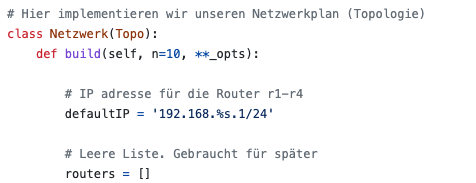
\includegraphics[width=0.6\textwidth]{Bilder/mininet1}
 \captionsetup{justification=centering,margin=1cm}
 \caption{Netzwerk-Klasse zur Topologie Erstellung}
 \label{mininet1}
\end{figure}

Im nächsten Teil der Klasse Netzwerk, werden die Komponenten des Netzwerks implementieren. Dies ist mit Hilfe einer Schleife mit 4 Durchläufen ausgeführt worden. Jeder Durchlauf entspricht einer Lokation, der jeweils einen Switch, einen Router und zehn Hosts erstellt. Dabei wird bei jeder Iteration erst ein Router-Objekt mit der Methode \textit{\textbf{self.addNode()}} erstellt, bei dem der Name, der private IP-Adressen-Bereich, die MAC-Adresse und der benutzerdefinierte Parameter für die Konfiguration, dass der Router IP-Forwarding aktiviert bekommt, übergeben. Danach wird der Router der vorher erstellten Liste eingefügt. Mit der Methode \textit{\textbf{self.addSwitch()}} wird ein Switch erstellt der einen Namen erhält. Anschließend wird mit der Methode \textit{\textbf{self.addLink()}} eine Verbindung zwischen dem Router und der Switch erstellt. Dabei wird auch die Netzwerkschnittstelle des Routers benannt und der private-IP-Adressenbereich vergeben  (siehe Abbildung \ref{mininet2}).

\begin{figure}[H]
 \centering
 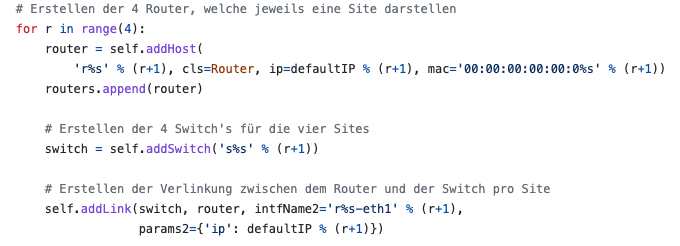
\includegraphics[width=0.7\textwidth]{Bilder/mininet2}
 \captionsetup{justification=centering,margin=1cm}
 \caption{Erstellung und Verbindung von Router und Switch}
 \label{mininet2}
\end{figure}

Danach folgt noch eine Schleife, bei der insgesamt n Hosts erstellt und mit dem Switch verbunden werden (siehe Abbildung \ref{mininet3}). Die Hosts erhalten für den jeweiligen privaten-IP-Bereich eine IP, eine MAC-Adresse und die IP des jeweiligen Routers als Standard-Route zugewiesen.
 
\begin{figure}[H]
 \centering
 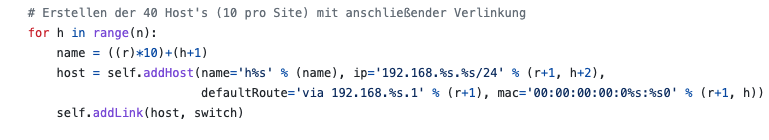
\includegraphics[width=0.8\textwidth]{Bilder/mininet3}
 \captionsetup{justification=centering,margin=1cm}
 \caption{Erstellung und Verbindung von Hosts und Switch}
 \label{mininet3}
\end{figure}

Nachdem für alle Lokationen der Rumpf erstellt worden ist, werden die Verbindungen zwischen den Routern mit dem Befehl \textit{\textbf{self.addLink()}} hergestellt. Dabei wird jeder Router mit allen anderen Routern verbunden. Dieser Vorgang wird das Internet simulieren, worauf ebenfalls der Tunnel und die Verschlüsselung implementiert wird. Dabei wird der Netzwerkschnittstellen-Name für beide Router und die jeweilige öffentliche-IP-Adresse definiert. Zusätzlich wird per \textit{\textbf{bw=20}} Befehl die Bandbreite der Leitung auf 20 Megabit gesetzt, wobei dies die geforderte SDSL-Leitung im Kapitel 3.8 darstellen soll (siehe Abbildung \ref{mininet4}).

\begin{figure}[H]
 \centering
 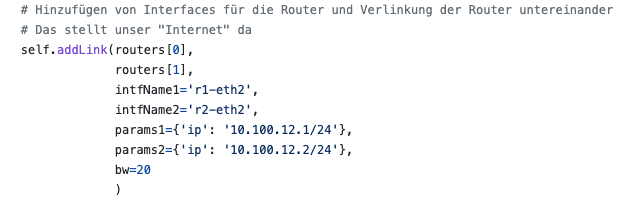
\includegraphics[width=0.7\textwidth]{Bilder/mininet4}
 \captionsetup{justification=centering,margin=1cm}
 \caption{Verbindung und Konfigurierung der Router}
 \label{mininet4}
\end{figure}




\newpage
\subsection{Controller Implementierung}
{\tiny Verfasst von: Tung, Mücahit\par}
Nach der Erstellung der Topologie geht es weiter bei der Main-Funktion. Es wird ein \textit{\textbf{RemoteController-Objekt}} erstellt, der einen Namen, die Konfiguration, um was für ein Controller es sich handelt, die IP-Adresse und den Port, wo er zu erreichen ist, bekommt (siehe Abbildung \ref{mininet5}). Hier ist wichtig zu erwähnen, dass der Controller auf Ubuntu läuft und zurzeit per \textit{\textbf{localhost}} zu erreichen ist. Der Controller könnte auf einer anderen VirtualBox-Maschine laufen und per \textit{\textbf{internes Netzwerk}} verbunden werden. Ebenfalls kann der Controller auf dem Hostsystem laufen und per \textit{\textbf{Host-Only-Adapter}} in Mininet eingebunden werden. 

\begin{figure}[H]
 \centering
 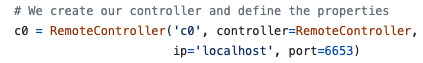
\includegraphics[width=0.7\textwidth]{Bilder/mininet5}
 \captionsetup{justification=centering,margin=1cm}
 \caption{Erstellung eines RemoteController's}
 \label{mininet5}
\end{figure}

Anschließend wird ein Mininet-Objekt erstellt, bei dem die erstellte Topologie, der erstellte Controller, ein \textit{\textbf{TCLink-Objekt}} für die Einstellung der Bandbreite der Netzwerkadapter und ein \textit{\textbf{OVSKernelSwitch-Objekt}} für die Erstellung der Switches als \textit{\textbf{Open vSwitches}} (siehe Abbildung \ref{mininet6}). Diese werden später verwendet, um den Quality of Service zu implementieren. Dabei werden per \textit{\textbf{ovs-vsctl-Befehle}} Queues an den Ports der Switches erstellt und die Priorisierung der Pakete vorgenommen.

\begin{figure}[H]
 \centering
 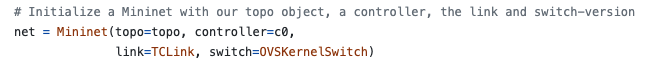
\includegraphics[width=1.0\textwidth]{Bilder/mininet6}
 \captionsetup{justification=centering,margin=1cm}
 \caption{Erstellung des Mininet-Objektes}
 \label{mininet6}
\end{figure}

\subsection{Ergebnis}
{\tiny Verfasst von: Tung\par}
Wenn das Mininet Skript ausgeführt wird, ist eine Topologie mit 40 Hosts über 4 Switches und 4 Routers zu sehen. Durch \textit{\textbf{pingall}} kann es festgestellt werden, dass alles richtig funktioniert hat (siehe Abbildung \ref{pingall}).

\begin{figure}[H]
 \centering
 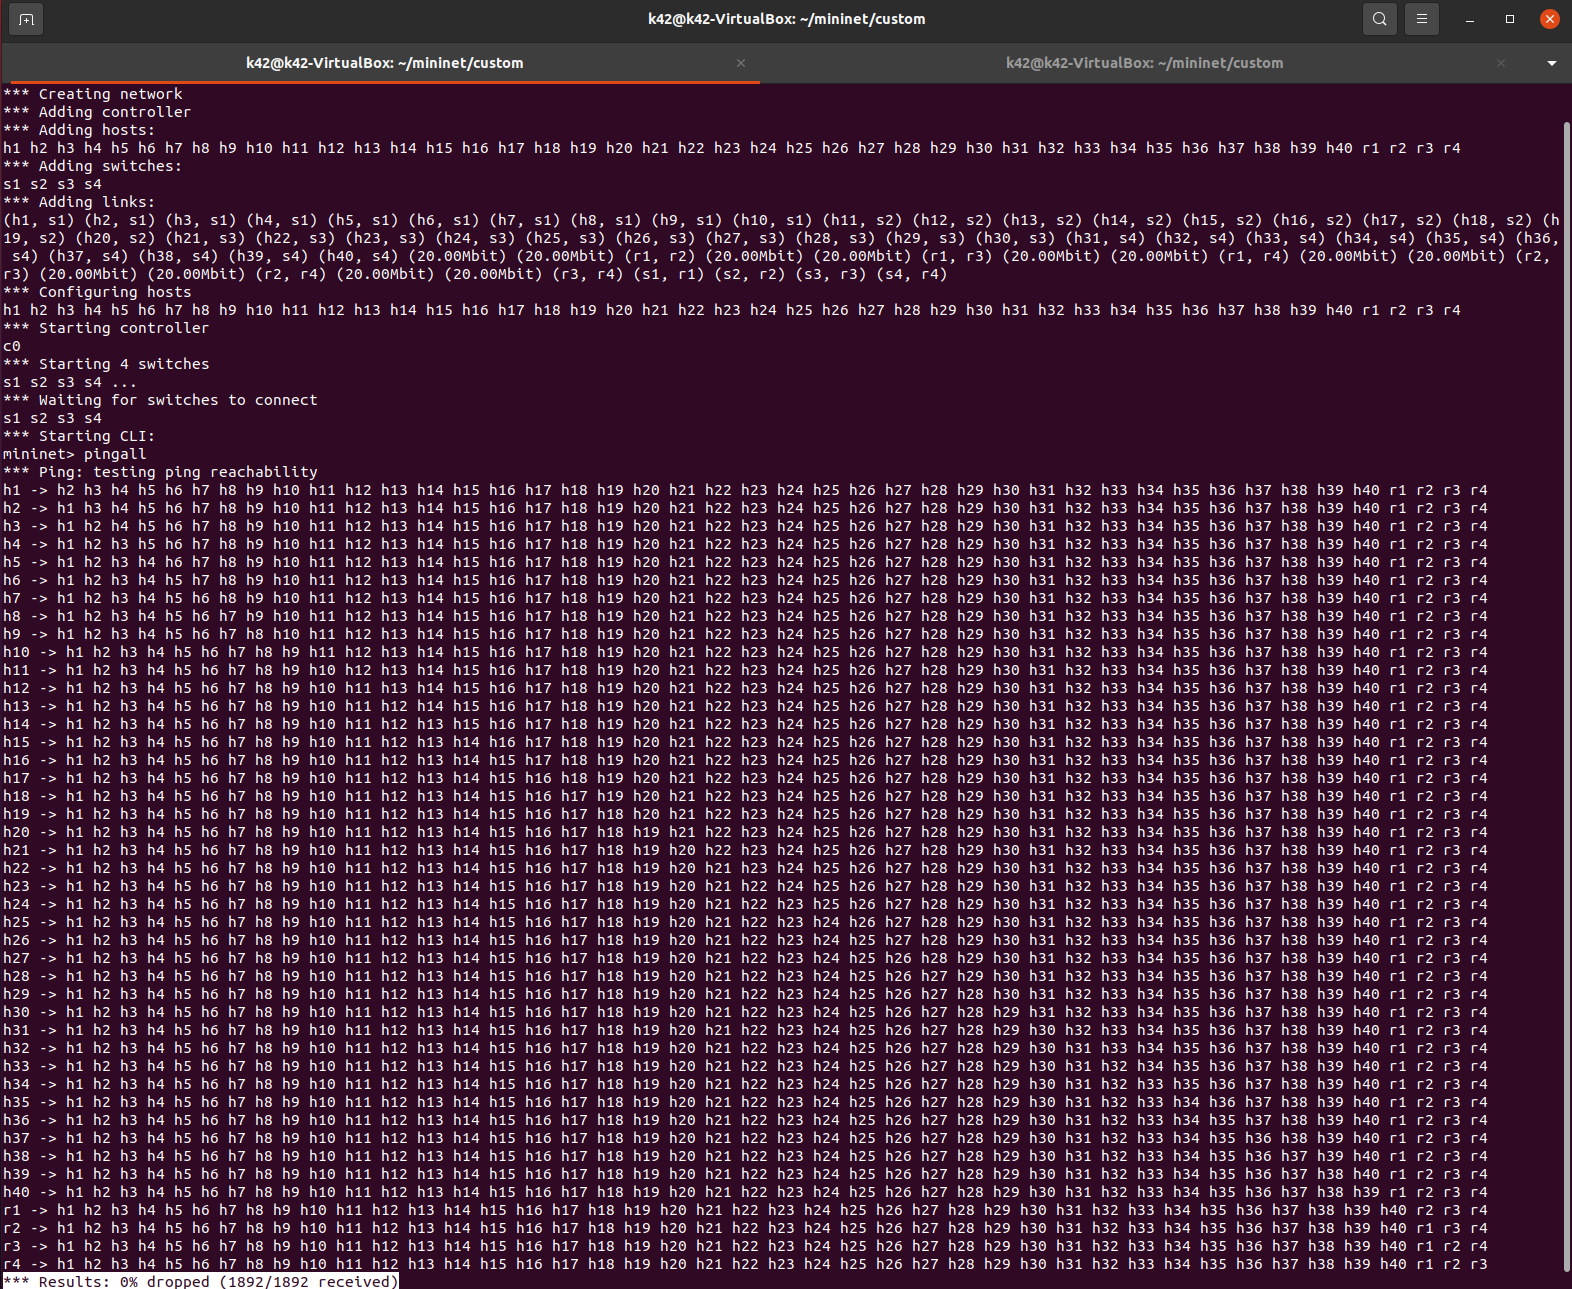
\includegraphics[width=1.0\textwidth]{Bilder/pingall}
 \captionsetup{justification=centering,margin=1cm}
 \caption{Ausführung und Testen vom Mininet-Skript}
 \label{pingall}
\end{figure}

\section{Verschlüsselung der Netzwerkverbindung zwischen den Lokationen}
{\tiny Verfasst von: Mücahit\par}
Zwischen den vier Lokationen soll ein Tunnel über das Internet konfiguriert werden. Dieser wird auch Virtual Private Network (VPN) genannt. Der gesamte Datenverkehr durch den Tunnel soll verschlüsselt und für unbeteiligte nicht einsehbar sein.

\subsection{Vorüberlegung}
{\tiny Verfasst von: Mücahit\par}
Der Tunnel wird zwischen den Routern r1-r4 entstehen und für eine Verbindung der Netzwerke der Lokationen sorgen. Damit soll eine \textit{\textbf{Site-to-Site-VPN}} Verbindung zwischen allen Lokationen hergestellt werden. Dieser zeichnet sich durch die Verschlüsselung ab den Schnittstellen, also den Routern der Lokationen, aus. Zudem werden aus dem privaten Netzwerk eingehende Pakete an den Routern verschlüsselt und weiterverschickt. Der Router an der Ziellokation wird das Paket entschlüsseln und an die Zieladresse weiterleiten. Die Methode, die implementiert werden soll, heißt \textit{\textbf{IPSEC over GRE}} und soll alle angestellten Vorüberlegungen ermöglichen.

\subsection{Durchführung}
{\tiny Verfasst von: Mücahit\par}
Für die Durchführung folgt in der Main-Funktion des Mininet-Skripts die Einrichtung der Tunnel zwischen den Routern beziehungsweise den Lokationen. Dafür baut jeder Router mit jedem Router einen GRE-Tunnel auf, für den der Befehl \textit{\textbf{ip tunnel add Tunnel-Name mode gre local Schnittstelle\hyp{}Router\hyp{}Lokation\hyp{}A remote Schnittstelle\hyp{}Router\hyp{}Lokation\hyp{}B ttl 255}} bei jedem Router über die Mininet-Methode \textit{\textbf{info(net[‘Router\hyp{}Name'].cmd(Befehl))}} ausgeben und ausgeführt wird (siehe Abbildung \ref{gre}). Nachdem die Verbindung definiert wurde, wird der Tunnel-Adapter per \textit{\textbf{ip link set Tunnel-Name up}} hochgefahren. Anschließend wird dem Tunnel Adapter mit dem Befehl \textit{\textbf{ip addr add Tunnel-IP dev Tunnel-Name}} die Tunnel IP vergeben. Hier ist wichtig, dass der IP-Adressbereich zwischen zwei Lokationen im selben Bereich liegt. Hier erfolgt das gleiche Prinzip wie bei der Erstellung und Simulierung des Internets zwischen den Lokationen.

\begin{figure}[H]
 \centering
 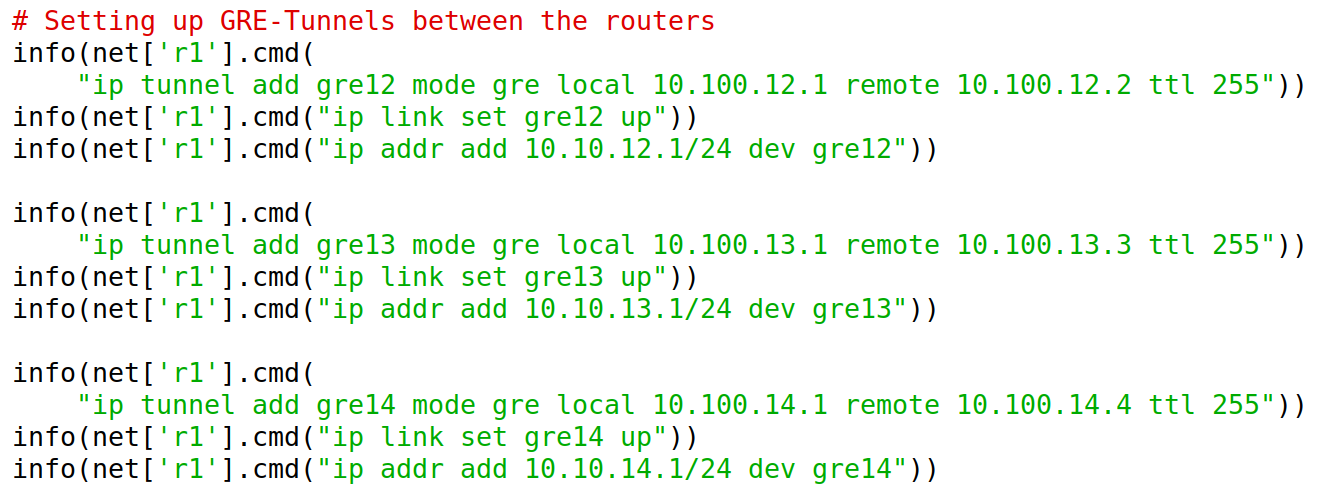
\includegraphics[width=1.0\textwidth]{Bilder/gre}
 \captionsetup{justification=centering,margin=2cm}
 \caption{Aufstellen der GRE-Tunnel}
 \label{gre}
\end{figure}

Nachdem der Tunnel aufgesetzt worden ist, sind alle Pakete, die durch den Tunnel versendet werden, nun als Payload eines neuen Paketes, wo der neue IP-Header der IP des Tunnels entspricht (siehe Abbildung \ref{ipsecgre}). Daraus folgt, dass nun Pakete, die die Maximum Transmission Unit (MTU) erreichen, jetzt eine geringere Länge annehmen müssen, da der neue Payload aus dem ursprünglichen Payload und IP-Header besteht. Wenn der Fall eintritt, schickt der Router eine Aufforderung an den Absender zurück, das Paket kleiner zu gestalten.

\begin{figure}[H]
	\centering
	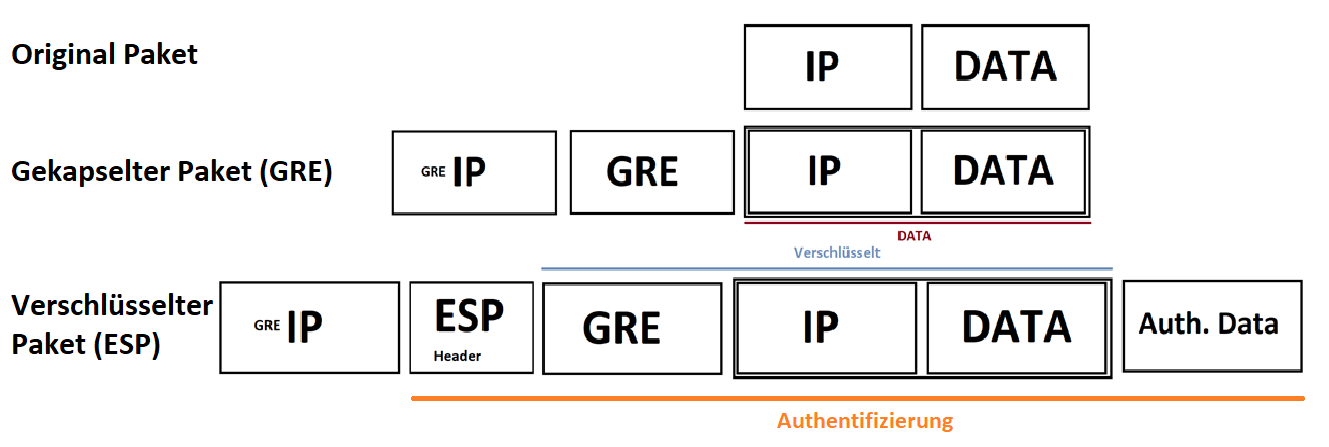
\includegraphics[width=1.0\textwidth]{Bilder/ipsecgre}
	\captionsetup{justification=centering,margin=2cm}
	\caption{Wandlung der Pakete bei IPSEC over GRE}
	\label{ipsecgre}
\end{figure}

Im nächsten Schritt wird die Route zum jeweils anderen Subnetzwerkadressenbereich per \textit{\textbf{ip route add IP-anderen-Lokation via IP-Adapter dev Adapter-Name}} Befehl in die Routing-Tabelle eingefügt (siehe Abbildung \ref{route}). Da es sich hierbei um eine Simulation handelt, sollten alle Lokationen einen jeweils anderen privaten Adressenbereich besitzen. Bei Überschneidungen könnte es zu Problemen führen. Bei einer echten Umgebung mit echten öffentlichen IP-Adressen könnten dieselben privaten IP-Adressen für verschiedene Lokationen genutzt werden. Dies wird in der Realität üblicherweise so gemacht.

\begin{figure}[H]
 \centering
 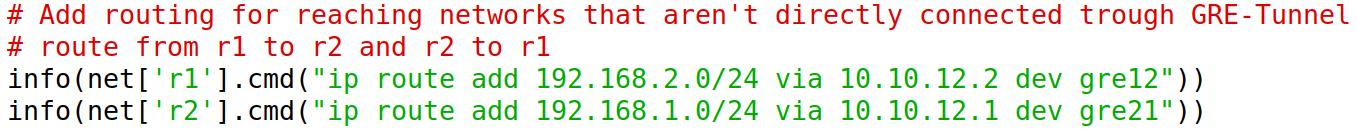
\includegraphics[width=1.0\textwidth]{Bilder/route}
 \captionsetup{justification=centering,margin=2cm}
 \caption{Konfiguration der Routen}
 \label{route}
\end{figure}


Der Tunnel von und zu den Lokationen ist nun aufgesetzt. Als Nächstes sollen alle Pakete aus dem privaten IP-Adressenbereich bei der Übermittlung durch den Router verschlüsselt und weitergeleitet werden. Dazu sollen alle Pakete von außen entschlüsselt und zum Zielort weitergeleitet werden. Für diese Methode wird die Verschlüsselung und Entschlüsselung über IPSEC im Transport-Modus mit dem Encapsulating Security Payload (ESP) Protokoll benutzt. Dafür wird zuerst der Befehl \textit{\textbf{ip xfrm state add src IP-Adresse-des-Routers dst IP-Adresse-des-Ziel-Routers proto esp Security-Parameter-Index-Key enc ‘cbc(aes)‘ 256bit-Key mode transport}} ausgeführt, um Regeln für die Ver- und Entschlüsselung auf dem Router einzufügen. Jeder Router bekommt zwei Regeln für jeweils einen anderen Router. Eine Regel ist für die Entschlüsselung bei ankommenden Paketen und die andere Regel für die Verschlüsselung bei abgehenden Paketen (siehe Abbildung \ref{state}).

\begin{figure}[H]
 \centering
 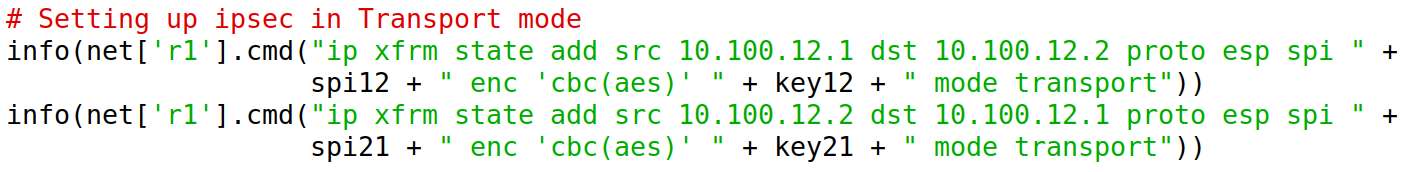
\includegraphics[width=1.0\textwidth]{Bilder/state}
 \captionsetup{justification=centering,margin=2cm}
 \caption{Erstellung der States für die Ver- und Entschlüsselung}
 \label{state}
\end{figure}

Der Befehl legt für Pakete mit bestimmter IP-Quelladresse, IP-Zieladresse, einem Security-Parameter-Index Key (SPI) und einer 256 Bit Verschlüsselung fest, bei einer Übereinstimmung das Paket zu verschlüsseln oder zu entschlüsseln. Auf Abbildung \ref{ipsecgre} kann der Wandel von der ursprünglichen Paketstruktur auf die verschlüsselte Paketstruktur nachvollzogen werden. Es wird für eingehende und ausgehende Pakete jeweils eine Regel festgelegt. Der Unterschied ist, dass die IP-Ziel- und Quelladresse, der Security-Parameter-Index-Key und die 256 Bit Verschlüsselung verschieden sind. Durch die States wurden die Ver- und Entschlüsselungen auf den Routern installiert. Die Keys und SPI’s wurden zufällig gewählt. 

Nun muss den Routern angewiesen werden, auf welchem Datenverkehr die installierten States angewandt werden sollen. Dies geschieht über Policies. Dort wird über den \textit{\textbf{ip xfrm policy add dir out src IP-Adresse-des-Routers dst IP-Adresse-des-Ziel-Routers tmpl proto esp mode transport}} Befehl die Anweisung erteilt, dass auf den IP-Ziel- und Quelladressen die Ver- und Entschlüsselung stattfinden soll. Dabei muss der Befehl zweimal eingegeben werden, wobei die IP-Adressen vertauscht werden (siehe Abbildung \ref{policy}). Es wird nicht die Tunnel-IP, sondern die Router-IP angegeben.

\begin{figure}[H]
 \centering
 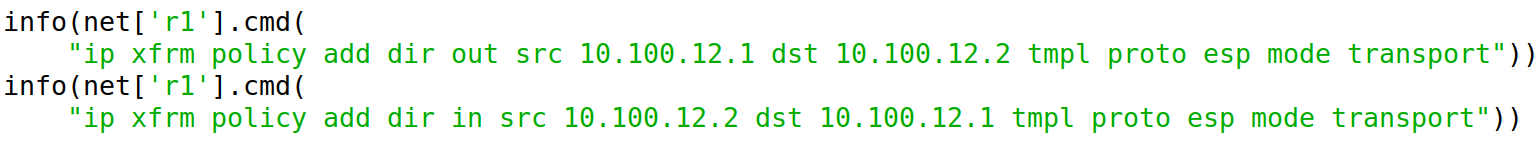
\includegraphics[width=1.0\textwidth]{Bilder/policy}
 \captionsetup{justification=centering,margin=2cm}
 \caption{Erstellung der Policies für die Ver- und Entschlüsselung}
 \label{policy}
\end{figure}

\subsection{Ergebnis}
{\tiny Verfasst von: Mücahit\par}
Durch die Erstellung der Tunnel und der Verschlüsselung der Pakete wurde die komplette Kommunikation zwischen den Lokationen sicherer. Dazu gehört unter anderem die Authentifizierung des Kommunikationspartners und der Verhinderung unautorisierter Veränderungen von Paketen. Zwischen den Lokationen war vorher der gesamte Datenverkehr ersichtlich, wohingegen jetzt nahezu alles verschlüsselt ist (siehe Abbildung \ref{esp}).

\begin{figure}[H]
 \centering
 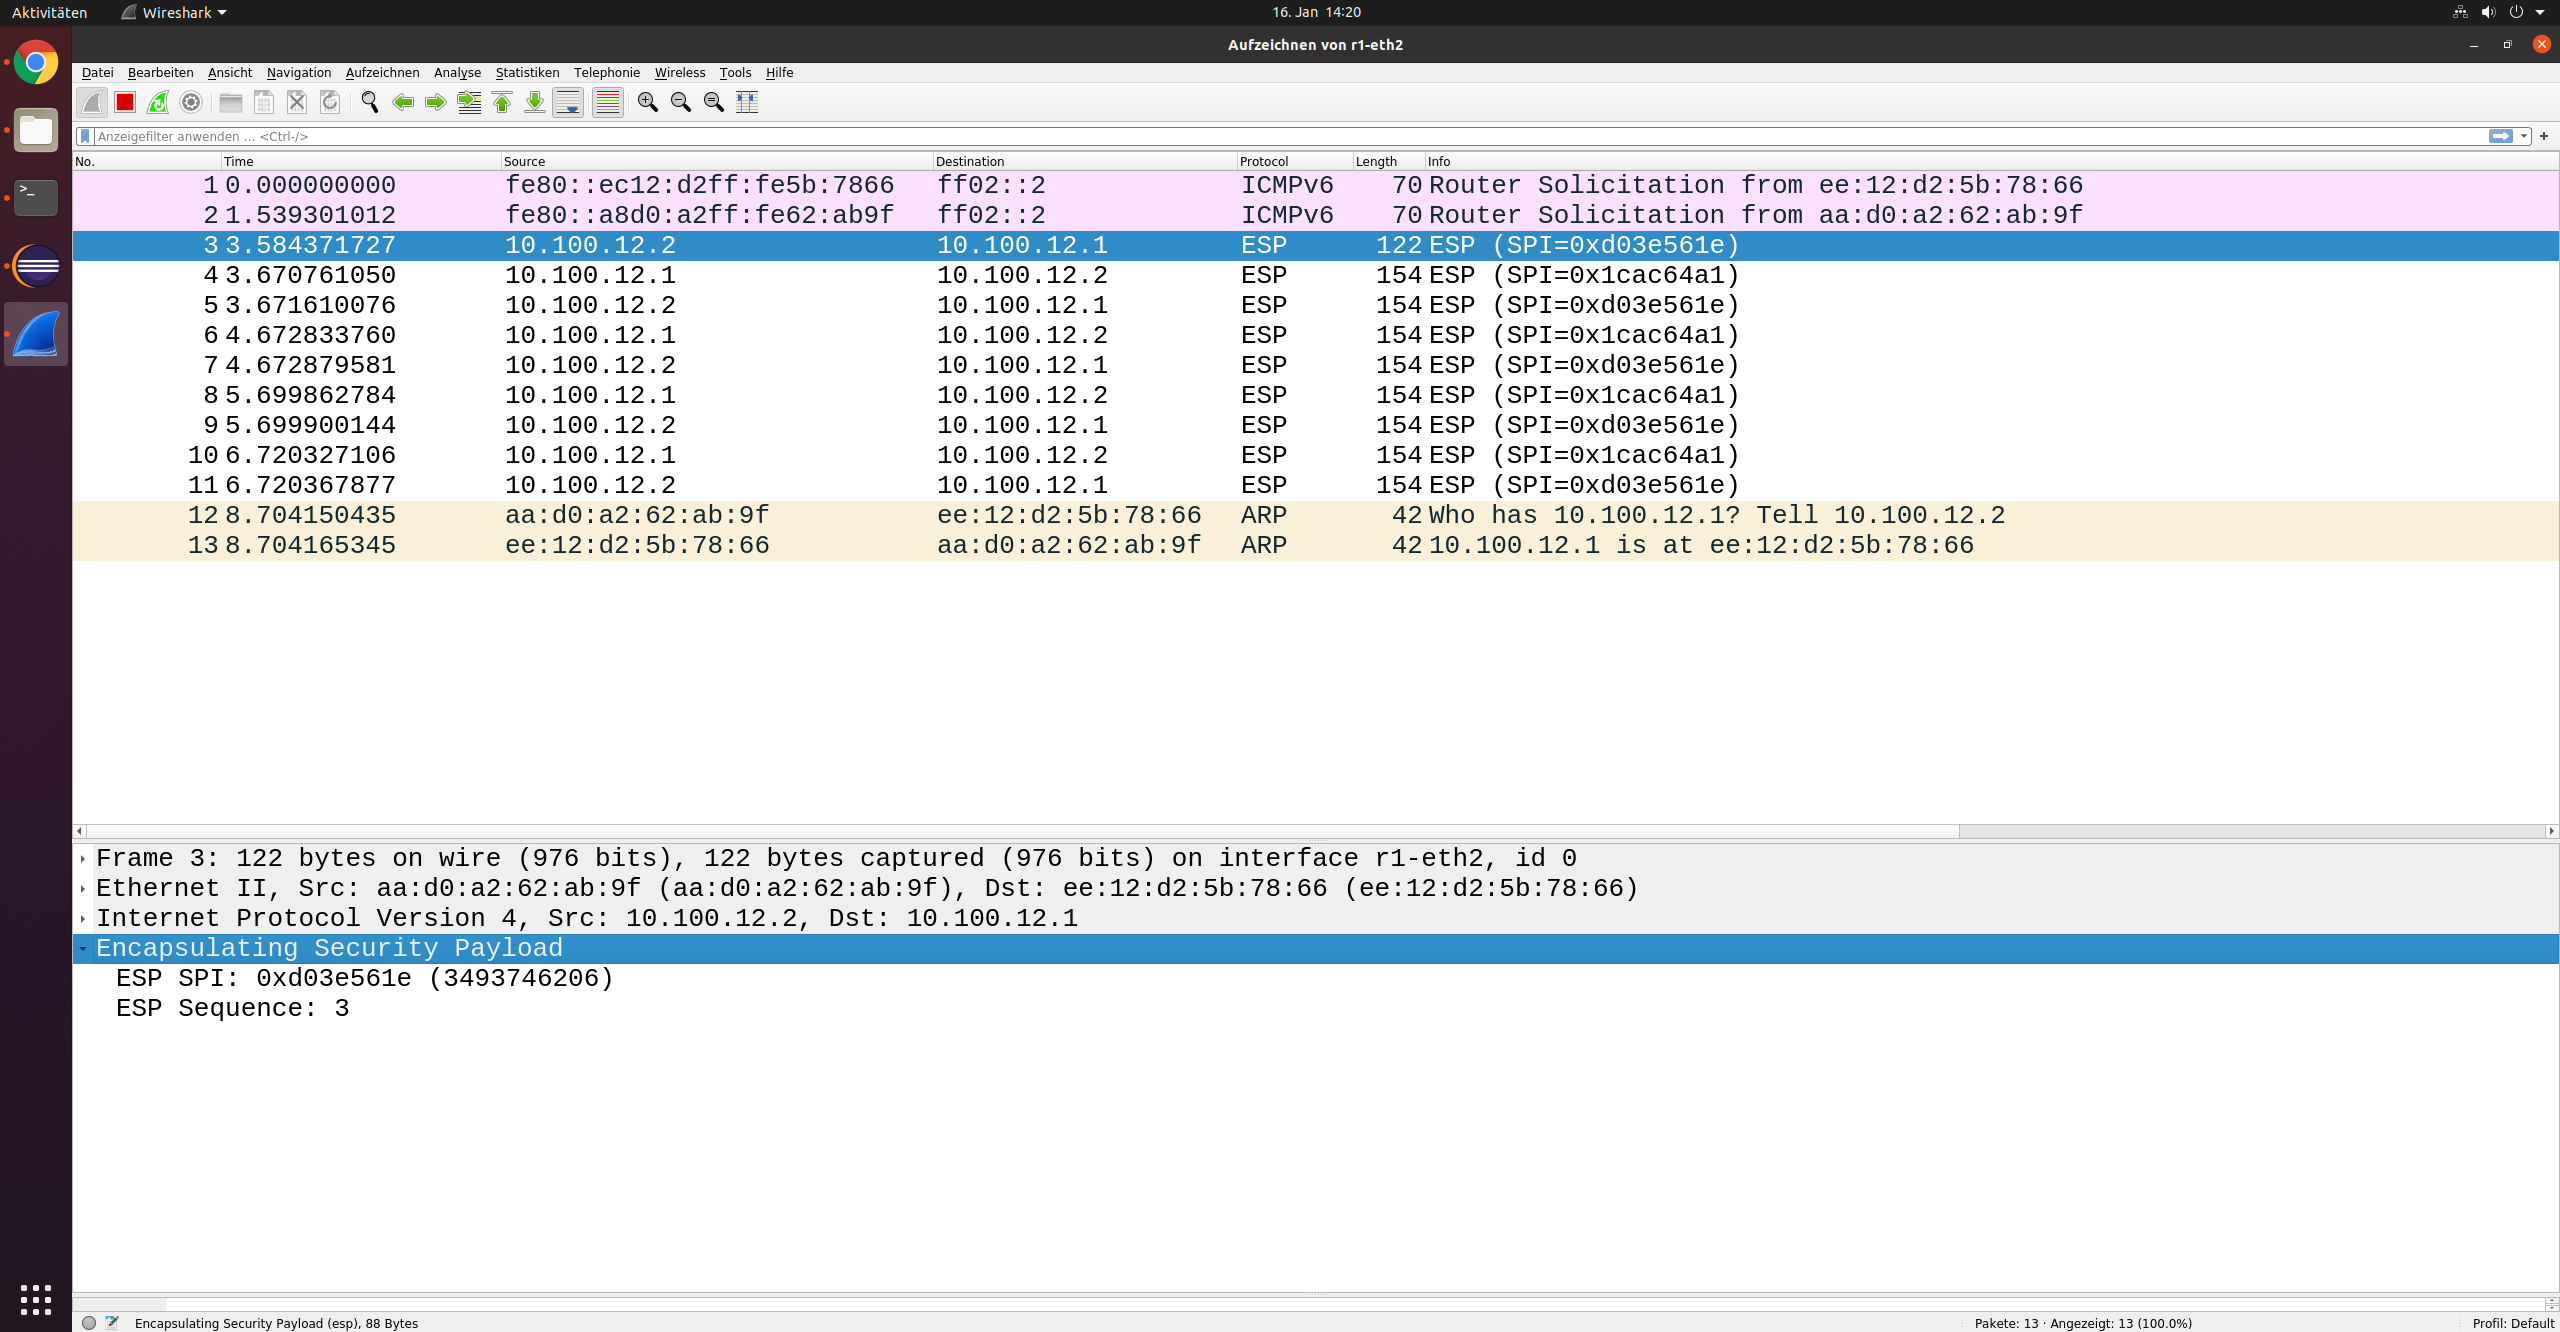
\includegraphics[width=1.0\textwidth]{Bilder/esp}
 \captionsetup{justification=centering,margin=2cm}
 \caption{Verschlüsselter Verkehr zwischen Standort Frankfurt und Berlin}
 \label{esp}
\end{figure}

\section{Auswahl des Service-Providers}
{\tiny Verfasst von: Tung, Naghmeh, James, Mücahit\par}
Alle Lokationen sind über einen Tunnel durch das Internet miteinander verbunden. Deswegen benötigen alle Lokationen eine DSL-Verbindung mit der richtigen Konfiguration zur Realisierung. Der Preis und die Bandbreite der DSL-Leitung zählen bei der Auswahl als primäre Faktoren. Zusätzlich können weitere Leistungen betrachtet werden. Im Folgenden sind in einer Tabelle die Internet-Service-Provider O2, Vodafone, 1\&1 und Telekom mit verschiedenen Bandbreiten und den dazugehörigen Nettopreisen aufgelistet (siehe Tabelle \ref{dsl}). Die Angebote sind aktuell und aus den originalen Webseiten der Provider entnommen worden.

\begin{table}[H]
\caption{DSL-Angebote verschiedener Internet-Service-Provider}
\label{dsl}
\centering
  \begin{tabular}{p{1.5cm} p{2.5cm} p{4cm} p{4cm} p{2.4cm}} 
\toprule
    Anbieter & Tarife & Download in Mbit/s (min/normal/max) & Upload in Mbit/s (min/normal/max)& Monatl. Preis (Netto, 24 Monate) \\
\midrule 
    	Telekom & Company Start 16 &  6,3 / 9,5 / 16 & 0,7 / 1,5 / 2,4 & 37 Euro\\
    	&Company Start 50&27,9 / 47 / 50&2,7 / 9,4 / 10& 42 Euro\\
	&Company Start 100&54 / 83,8 / 100&20 / 33,4 / 40& 47 Euro\\
	&Company Start 250&175/ 200 / 250&20 / 35 / 40& 57 Euro\\
	&Company Start 500&400 / 500/ 500&80/ 100/ 100& 70 Euro\\
	&Company Start 1000&700/ 850 / 1000&200 / 200 / 200& 100 Euro\\
	1\&1	&DSL 16	&6,6 / 11 / 16	&0,128 / 0,983 / 1		& 20 Euro\\
 	&DSL 50	&16,7/ 44 / 50&	1,6 / 9,6 / 10&		22,5 Euro\\
 	&DSL 100	&54 / 88,6 / 100	&20 / 36,9 / 40&		25 Euro\\
 	&DSL 250&	175/ 200/ 250	& 20 / 35 / 40		& 30 Euro\\
	&Glasfaser 500&	431/ 250/ 480	 &215/ 225/ 240	&	200 Euro\\
 	&Glasfaser 1.000&	860/ 900/ 1000	&430/ 450/ 500&	350 Euro\\
	Vodafone& Plus 16 Regio DSL&	6 / 9,5 / 16&	0,7 / 0,9 / 1&		20 Euro\\
 	&Plus 50 Regio DSL&	28 / 38 / 50&	2,7 / 7,5 / 10&		22,5 Euro\\
 	&Plus 100 Regio DSL&	54 / 87/ 100&	20 / 37 / 40&		25 Euro\\
 	&Plus 250 Regio DSL&	175/ 210/ 250& 	20/ 37/ 40	&	30 Euro\\

	
	O2 &MyOffice S&	0,3/ 8 / 10	& 0,3 / 1,5 / 2&		25 Euro\\
 	&MyOffice M&	3/ 38 / 50&	0,7 / 8 / 10&		27,5 Euro\\
 	&MyOffice L&	50/ 83/ 100&	10 / 33/ 40&		30 Euro\\
 	&MyOffice XL&	105/ 200 / 250&	12/ 33 / 40&		35 Euro\\

  \end{tabular}

\end{table}


Die notwendige Bandbreite für den Download und Upload wurde in der Gruppe abgestimmt. Vorher wurden kleine Tests zur Belegung und Stärkung der Argumente für die Abstimmung gemacht. Bei der Abstimmung wurde pro Arbeitsplatz mindestens 10 Megabit als Download und 5 Megabit als Upload für einen flüssigen Arbeitsrhythmus als notwendig gesehen. Demnach sind bei zehn Arbeitsplätzen ein Upload von mindestens 50 Megabit und ein Download von mindestens 100 Megabit nötig. Nach dem Preisleistungsverhältnis ist der Telekom Company Start 500 Angebot mit einer garantierten Uploadrate von mindestens 80 Megabit und einer garantierten Downloadrate von mindestens 400 Megabit die beste Wahl. Zusätzlich besitzt die Telekom jahrelange Erfahrung und beweist dadurch gute Qualitäten, welches die Entscheidung für das Produkt noch einmal gestärkt hat.\par
Neben einer DSL-Leitung benötigen die Lokationen eine Standleitung. Eine Standleitung ist sicherer als das Internet, weil der Datenverkehr über eine private Leitung verläuft. Es ist im Rahmen des Möglichen, dass bei der Leitung physikalisch von außen Pakete abgefangen werden können. Standleitungen sind meistens symmetrisch ausgelegt und besitzen die gleiche Uploadrate wie die Downloadrate. Die Preise für Standleitungen gibt es bei Service-Providern erst nach einer Anfrage mit der Angabe der Adressen der Lokationen. Demnach ist eine genauere Preisangabe nicht möglich. Die Kosten für eine Standleitung aller vier Lokationen würde nach Recherchen bei einer symmetrischen Geschwindigkeit von 100 Megabit ungefähr zwischen 500 und 1100 Euro liegen. Die Spanne zwischen den Preisen ist groß, da Preise sich selbst von Gebäude zu Gebäude ändern. Infolgedessen ist für einen genaueren Preis eine Anfrage unabdingbar.


\section{Einrichtung des NAT-Firewalls}
{\tiny Verfasst von: Mücahit\par}
Durch die Network Address Translation (NAT) Firewall Funktion werden private IPv4-Adressen beziehungsweise Geräte geheim gehalten. Es wird durch die Netzwerkadressenübersetzung keine Informationen über die privaten IPv4-Adressen ins World Wide Web geschickt. Dazu wird der IPv4-Header von IP-Paketen aus dem privaten Netzwerkbereich auf die öffentliche IPv4-Adresse verändert. Hinter jeder öffentlichen IPv4-Adresse können mehrere Tausende Geräte stehen und auf das Internet zugreifen. Des Weiteren ist die Anzahl der IPv4-Adressen durch den eigenen Aufbau begrenzt. Für die vier Lokationen würde der Internet-Service-Provider vier öffentliche IPv4-Adressen vergeben. Die Adressen werden vom Internet-Service-Provider in bestimmten Zeitintervallen immer wieder neu vergeben, welches ebenfalls zu einer gewissen Sicherheit beiträgt.

\subsection{Vorüberlegung}
{\tiny Verfasst von: Mücahit\par}
Die NAT-Firewall Funktion muss am Router einer Lokation implementiert werden, da alle Hosts über ihn Anfragen ins Internet verschicken werden. Dazu sollte jede Anfrage ins World Wide Web mit der öffentlichen IPv4-Adresse des Routers durchgeführt werden. Zusätzlich sollte der Router beziehungsweise die Hosts den Dynamic-Name-Server (DNS) konfiguriert bekommen, damit die Hosts nicht nur über die IPv4-Adressen aufs Internet zugreifen.

\subsection{Durchführung}
{\tiny Verfasst von: Mücahit\par}
\begin{wrapfigure}{R}{0.5\textwidth}
	\vspace{-\baselineskip}
 	\centering
 	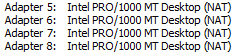
\includegraphics[width=0.5\textwidth]{Bilder/adapter}
 	\captionsetup{justification=centering}
 	\caption{VirtualBox NAT-Adapter}
	\label{adapter}
\end{wrapfigure}

Um den Hosts der Lokationen den Internetzugang zu ermöglichen, muss zuerst den Routern der Zugang zum Internet möglich sein. Dafür wurde in VirtualBox die vier Netzwerk-Adapter für die vier vorgesehenen Lokationen aktiviert und als NAT konfiguriert (siehe Abbildung \ref{adapter}). 
Die vier Schnittstellen wurden jeweils an die Router r1, r2, r3 und r4 per \textit{\textbf{Intf(„Schnittstellenbezeichnung“, node=Router-Objekt)}} Befehl zugewiesen. Die Schnittstellenbezeichnung kann vorher mit dem Befehl \textit{\textbf{ifconfig -a}} angezeigt werden. Die Router-Objekte werden vorher per \textit{\textbf{variabel = net.getNodeByName('Router-Bezeichnung')}} Befehl instanziiert. Jeder Router bekommt eine individuelle Schnittstelle zugewiesen. Die Router führen anschließend den \textit{\textbf{info(net['Router-Bezeichnung].cmd("dhclient Schnittstellenbezeichnung"))}} Befehl aus, um eine IPv4-Adresse des VirtualBox NAT-Services zu erhalten (siehe Abbildung \ref{interface}). Der IPv4-Adressenbereich, der vom NAT-Service vergeben wird, liegt bei \textit{\textbf{10.0.X.X/24}} und ändert sich je nach virtueller Maschine.

\begin{figure}[H]
 \centering
 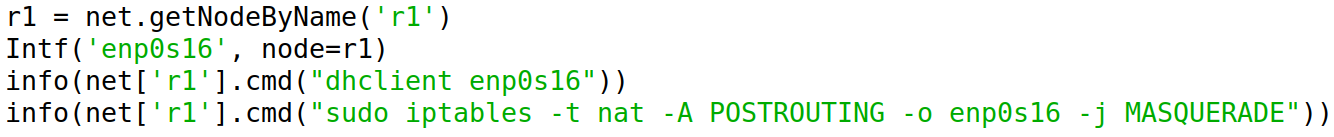
\includegraphics[width=1.0\textwidth]{Bilder/interface}
 \captionsetup{justification=centering,margin=2cm}
 \caption{Einbindung und Konfigurierung des NAT-Adapters}
 \label{interface}
\end{figure}

Da nun eine Internetverbindung für alle Router besteht, muss der Domain Name System Server auf dem Ubuntu-Host festgelegt werden, damit die Hosts nicht nur per IPv4 auf das Internet zugreifen können. Eine Möglichkeit besteht darin, die Datei \textit{\textbf{/etc/resolv.conf}} per Admin-Rechte zu bearbeiten und dort den Domain Name System Server festzulegen. Es kann der Domain Name Server von Google mit der IPv4 \textit{\textbf{8.8.8.8}} und/oder \textit{\textbf{8.8.4.4}} eingetragen werden. Ein Nachteil bei der Variante ist, dass nach jedem Neustart des Betriebssystems dieser Vorgang erneut durchgeführt werden muss, da der Eintrag nur temporär bis zum Ausschalten des Betriebssystems erhalten bleibt. Um dem entgegenzuwirken wurde das Paket Resolvconf per \textit{\textbf{sudo apt install resolvconf}} installiert. Dadurch wurden neue Dateien in der Konfigurationsebene von Ubuntu erstellt, wodurch ein permanenter Eintrag des DNS Servers möglich war. Dafür wurde die IPv4 des DNS Server in die Datei \textit{\textbf{/etc/resolvconf/resolv.conf.d/head}} eingetragen und gespeichert. Anschließend wurde der Netzwerkmanager per \textit{\textbf{sudo systemctl restart network-manager}} Befehl neu gestartet, um die Einstellungen zu übernehmen. Jetzt ist es den Routern möglich, das Internet auch per Domainnamen zu erreichen.

Die Default-Route der Hosts ist der jeweilige Router in der Lokation. Wenn ein Host eine Website aufruft, schickt er eine Anfrage an und über den Router. Im Moment wird die Anfrage beim Router fallengelassen, da der Router noch keine Regeln bezüglich solcher Anfragen besitzt. Die Regel wird über das im Ubuntu vorhandene Programm \textit{\textbf{iptables}} eingetragen, welches den Linux-Kernel umkonfiguriert. Dazu wird auf allen Routern der Befehl \textit{\textbf{sudo iptables -t nat -A POSTROUTING -o Schnittstellenbezeichnung -j MASQUERADE}} ausgeführt. Der Befehl vergibt jedem eingehenden Paket als Quelladresse die IPv4-Adresse der NAT-Schnittstelle des Routers (siehe Abbildung \ref{adapter}). Es wird \textit{\textbf{MASQUERADE}} genutzt, weil zum Zeitpunkt der Ausführung des Befehls die IPv4-Adresse der Schnittstelle unbekannt sein beziehungsweise sich ändern kann. Bei einer statischen IPv4-Adresse der NAT-Schnittstelle würde statt MASQUERADE direkt die IP eingegeben werden.

\subsection{Ergebnis}
{\tiny Verfasst von: Mücahit\par}
Zusammenfassend wurde die NAT-Firewall-Funktion an allen Lokationen konfiguriert. Den Hosts ist es nun möglich, Anfragen ins Internet zu versenden. Der Router führt die Anfragen mit der von VirtualBox zur Verfügung gestellten Schnittstelle aus und gibt dem Host die Antwort zurück (siehe Abbildung \ref{nat}).

\begin{figure}[H]
 \centering
 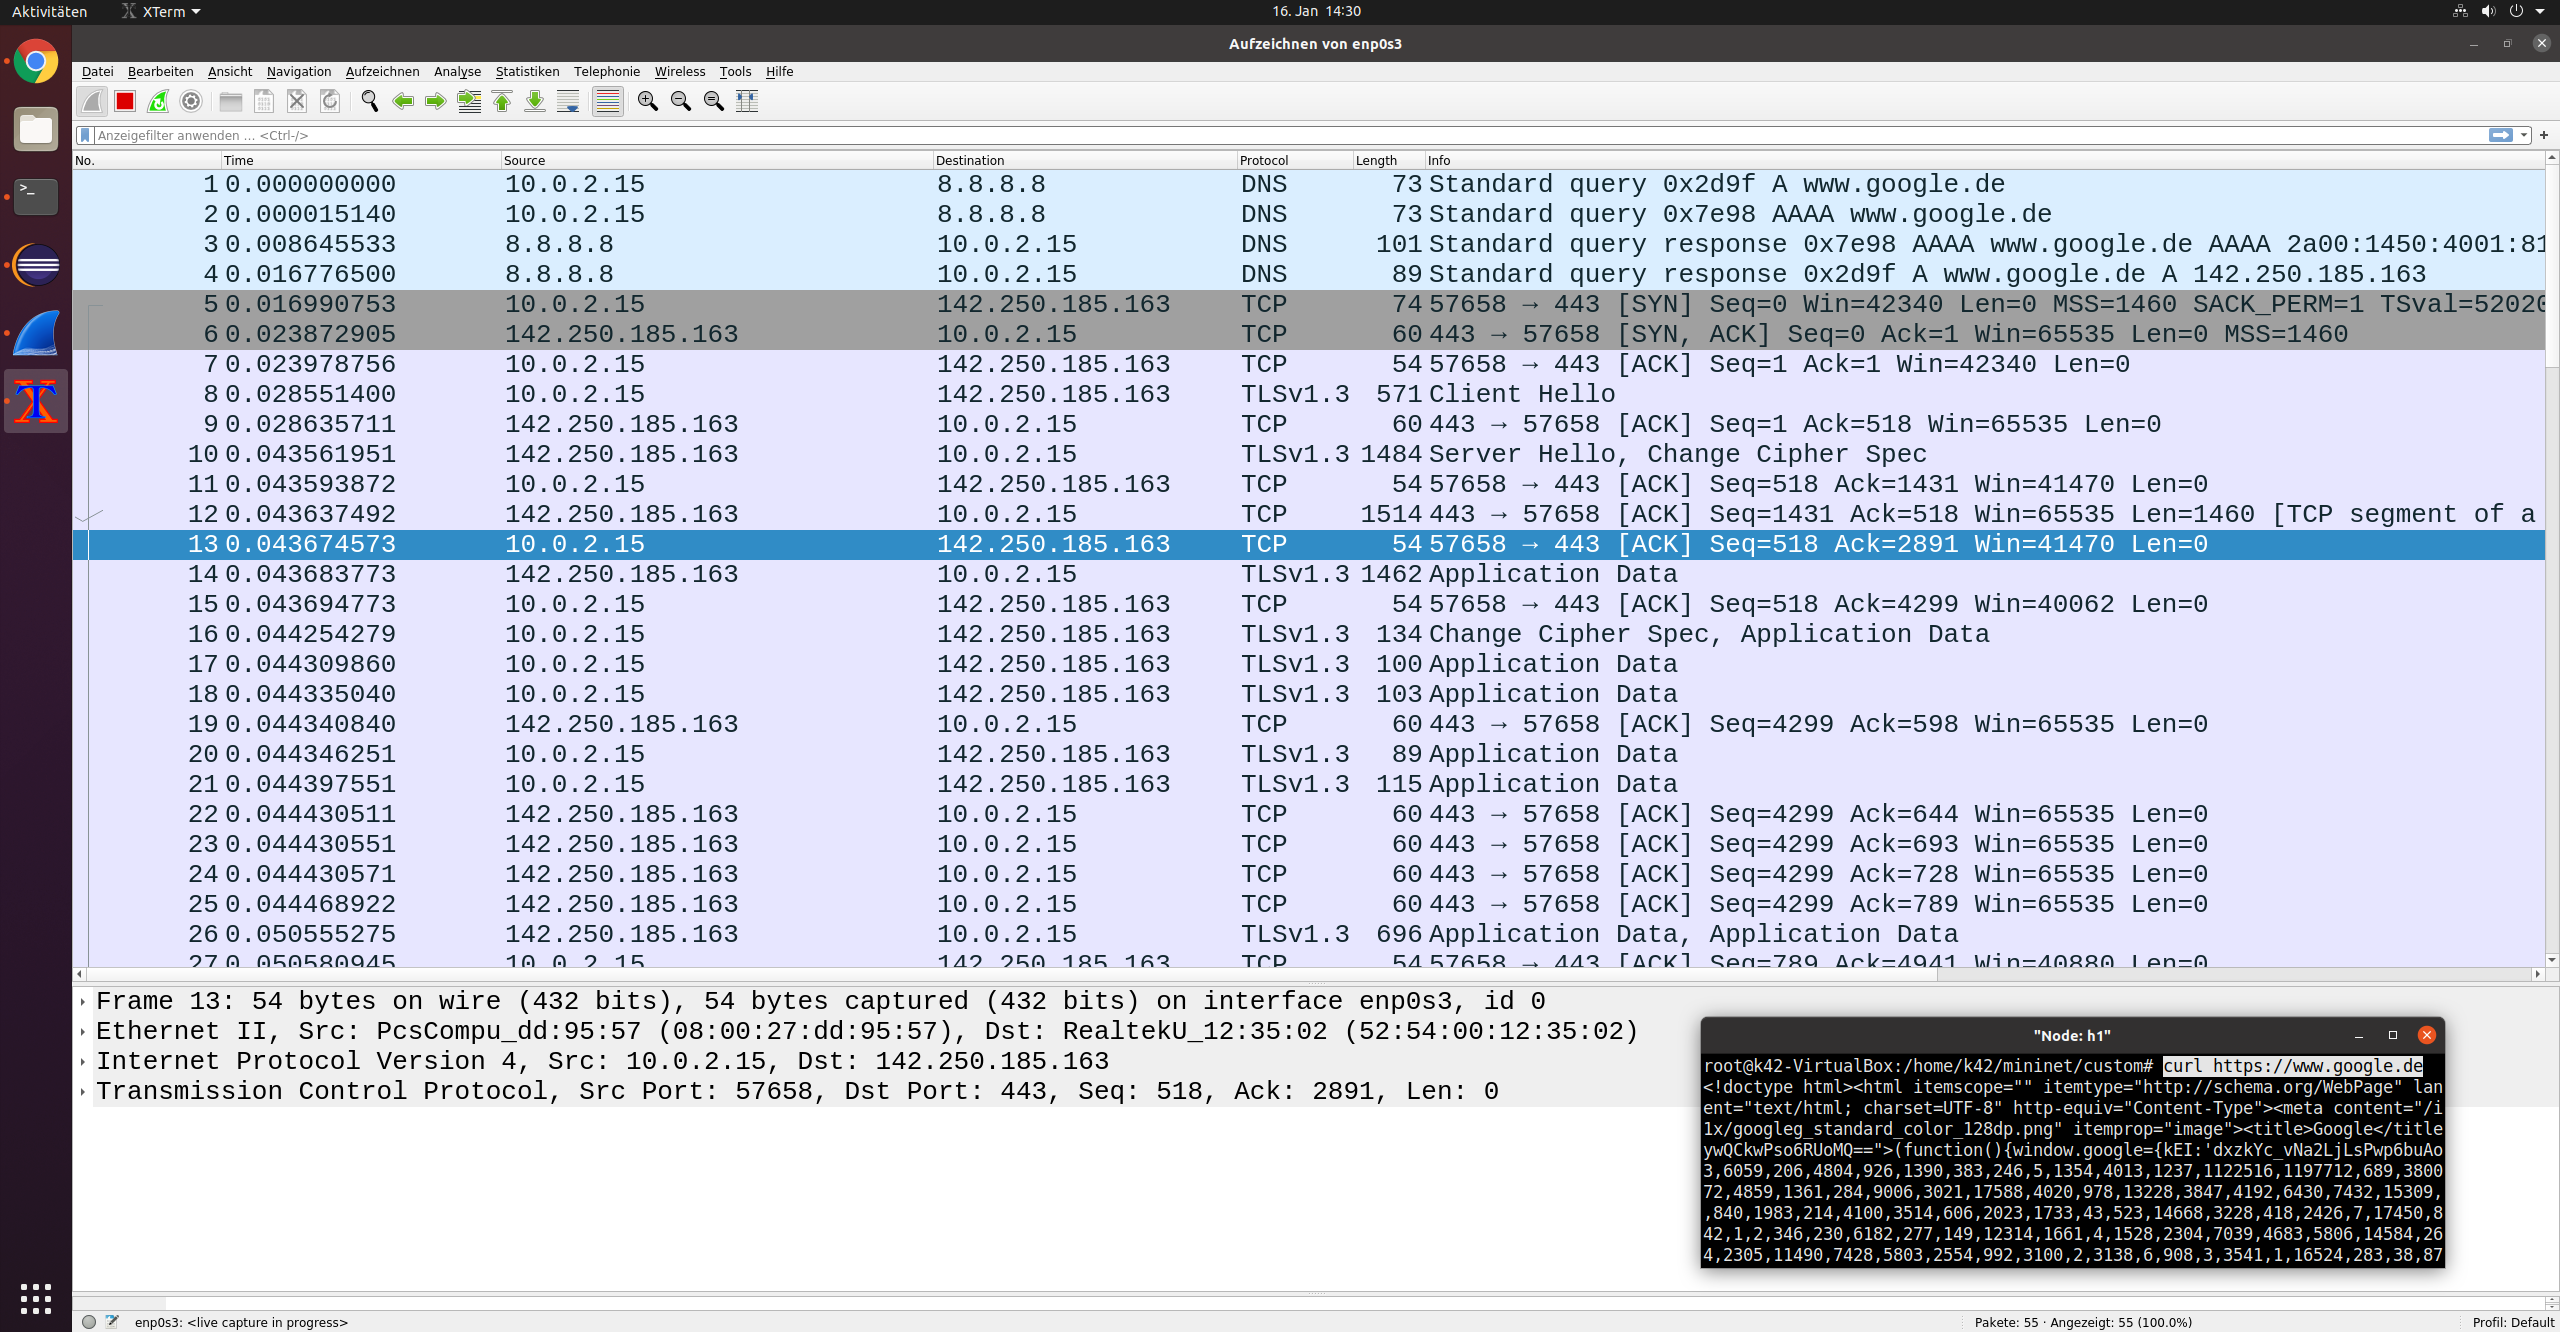
\includegraphics[width=1.0\textwidth]{Bilder/nat}
 \captionsetup{justification=centering,margin=2cm}
 \caption{Anfrage von H1 wird über Public IP des Routers durchgeführt}
 \label{nat}
\end{figure}

Ein Problem bei der Durchführung war, dass die Netzwerkschnittstellen beim Beenden von Mininet auch für Ubuntu nicht mehr verfügbar waren. Deshalb musste immer wieder die virtuelle Maschine beziehungsweise Ubuntu neu gestartet werden, wenn Mininet beendet wurde. Um dem entgegenzuwirken, wurde der Befehl \textit{\textbf{ip link set Schnittstellenbezeichnung netns 1}} im Mininet-Script kurz vor dem Beenden eingefügt, damit die Schnittstelle erneut für Ubuntu verfügbar war.

\section{Implementierung der Webproxy-Funktion}
{\tiny Verfasst von: Mücahit\par}
Der Proxy übernimmt jede Hypertext Transfer Protocol (HTTP) und Hypertext Transfer Protocol Secure (HTTPS) Anfrage der Hosts, führt sie selber durch und leitet die Antwort dem ursprünglichen Host wieder zurück. Der Vorteil hierbei ist, dass der Web-Proxy-Server für eine Sicherheit in allen Schichten des OSI-Modells sorgen kann. Es muss lediglich nur an dem Web-Proxy-Server Einstellungen bezüglich gewünschter Inhalte, IP-Adressen oder MAC-Adressen vorgenommen werden. Damit ist die Sicherheit für alle Geräte gewährleistet, die über den Web-Proxy-Server Anfragen verschicken. Des Weiteren wäre die Bandbreite weniger ausgelastet, da der Web-Proxy-Server jede neue Antwort in seinem Cache speichert. Bei gleicher Anfrage in einem benutzerdefinierten Zeitintervall wird die Antwort aus dem Cache statt durch erneute Anfrage ins Internet ausgegeben.

\subsection{Vorüberlegung}
{\tiny Verfasst von: Mücahit\par}
Für eine Webproxy-Funktion muss in allen Lokationen ein Webproxy-Server eingerichtet werden. Hosts müssen ohne vorher konfiguriert zu werden, Anfragen über den Proxy versenden können, wenn sie neu an das Netzwerk hinzukommen. Dem Host ist nicht bewusst, dass seine Anfragen über einen Proxy laufen. Anfragen würden über den Switch an den Webproxy weitergeleitet werden. Dieser führt die Anfrage durch und gibt dem Host die Antwort zurück. Die Umleitung sollte durch den Controller konfiguriert werden. 

\subsection{Durchführung}
{\tiny Verfasst von: Mücahit\par}
Um die Webproxy-Funktion zu realisieren, wurde in allen Lokationen jeweils ein weiterer Host in Mininet konfiguriert. Es wurde allen eine IPv4-Adresse im privaten Netzwerkadressenbereich vergeben und mit dem dazugehörigen Switch verbunden. Diese Hosts sollen nun als Webproxy-Server dienen. Es wurde zunächst per \textit{\textbf{Xterm Proxybezeichnung}} Befehl ein externes Terminal gestartet und die Internetverbindung durch das Aufrufen einer beliebigen Website als funktionsfähig getestet. Dazu wurde das Kommandozeilenprogramm \textit{\textbf{cURL}} verwendet, welcher vorher per \textit{\textbf{sudo apt install curl}} installiert werden muss.
Als Nächstes sollte eine weitere Schnittstelle des Webproxy-Servers mit einer Schnittstelle von VirtualBox verbunden werden. Dieser sollte dann als Bridge zwischen zwei VirtualBox-Maschinen genutzt werden. Auf der zweiten VirtualBox-Maschine sollte das Programm Squid installiert werden. Im Gesamtbild sollte eine Anfrage eines Hosts über den Proxy-Server auf eine andere VirtualBox-Maschine weitergeleitet, dort durchgeführt und die Antwort anschließend zurückgeleitet werden. Leider scheiterte dieser Versuch, da bei der Haupt-VirtualBox-Maschine der Promiscuous-Modus des Netzwerkbrückenadapters auf deny eingestellt war. Dadurch konnte keine gescheite Verbindung zwischen den zwei VirtualBox-Maschinen hergestellt werden. Aus diesem Grund haben wurde ein alternativer Proxy-Skript aus Github benutzt, um die Webproxy-Funktionalität direkt auf dem Host beziehungsweise Server einzurichten. Dazu wurde per Xterm ein Terminal gestartet und das Skript ausgeführt. Dieser nimmt nur HTTP Anfragen entgegen, führt sie selber durch und gibt für einen bestimmtes Zeitintervall die Antworten aus dem Cache zurück. Hier ist noch mal zu verdeutlichen, dass das Python-Skript für keine umfangreiche Web-Proxy-Funktionalität ausgelegt ist, jedoch dieser aus Testzwecken benutzt wurde. Als Nächstes wurden alle Pakete, die beim Switch eingehen und einen Ziel-Port als 80 besitzen, an den Proxy weitergeleitet. Hierfür wurde über den Controller die entsprechenden Flows als Match eingetragen, die dazugehörigen Actions implementiert und dem Switch die Anweisungen geschrieben. Dadurch bekommt der Webproxy-Server die Anfragen der Hosts, ohne dass die Geräte umkonfiguriert werden müssen. Der Proxy nimmt die Anfrage entgegen, führt sie selber durch und gibt die Antwort an das jeweilige Gerät weiter. Hier tritt das Problem auf, dass das Gerät eine Antwort von der Website erwartet, jedoch die Antwort vom Proxy geschickt bekommt. Die Antwort des Proxys könnte ebenfalls per Controller modifiziert und an das jeweilige Gerät weitergeleitet werden. Jedoch fehlte die Information des Absenders aus dem Internet zu dem Zeitpunkt, an dem die Antwort vom Proxy an den Host geschickt wurde.

\subsection{Ergebnis}
{\tiny Verfasst von: Tung, Naghmeh, James, Mücahit\par}
Resultierend war es nicht möglich, die Webproxy-Funktion zu implementieren. Alternativ könnte eine transparente Web-Proxy-Funktion an dem Router der jeweiligen Lokationen eingerichtet werden. Dieser führt die Anfragen selber durch, speichert und sendet die Antwort an den jeweiligen Host zurück. Auch das Eintragen des Proxyservers an den jeweiligen Hosts, die mit dem Switch verbunden sind, würde sich als funktionsfähig erweisen. Diese Art wird direkter Proxy genannt und trägt viel Aufwand mit sich.

\section{Aufbau eines zentralen Topologie-Viewers und einer Monitoring-Lösung}

\subsection{Topologie}
{\tiny Verfasst von: Mücahit\par}
Die Topologie unseres Netzwerkes kann auf dem Web User Interface des Floodlight-Controllers eingesehen werden. Ein mit der Standardinstallation geliefertes Floodlight-Modul stellt die Information der Topologie in einer Weboberfläche zur Verfügung. Zum Einsehen der Topologie muss auf einem Webbrowser die Benutzeroberfläche des Controllers über den Link \textit{\textbf{http://<controller-ip>:8080/ui/index.html}} aufgerufen werden. Anschließend wird auf dem linken Reiter die Option Topology angeklickt, wodurch die Topologie angezeigt wird (siehe Abbildung \ref{topo}). Durch die Benutzung einer VirtualBox werden vier getrennte Topologien angezeigt. Die Verbindungen zwischen den Routern werden bei der Visualisierung vom Controller ignoriert. Dies schränkt jedoch nicht die Funktionsweise des Netzwerkes ein. Bei der Nutzung vier getrennter VirtualBox-Maschinen, würde die Topologie korrekt dargestellt werden.

\begin{figure}[H]
 \centering
 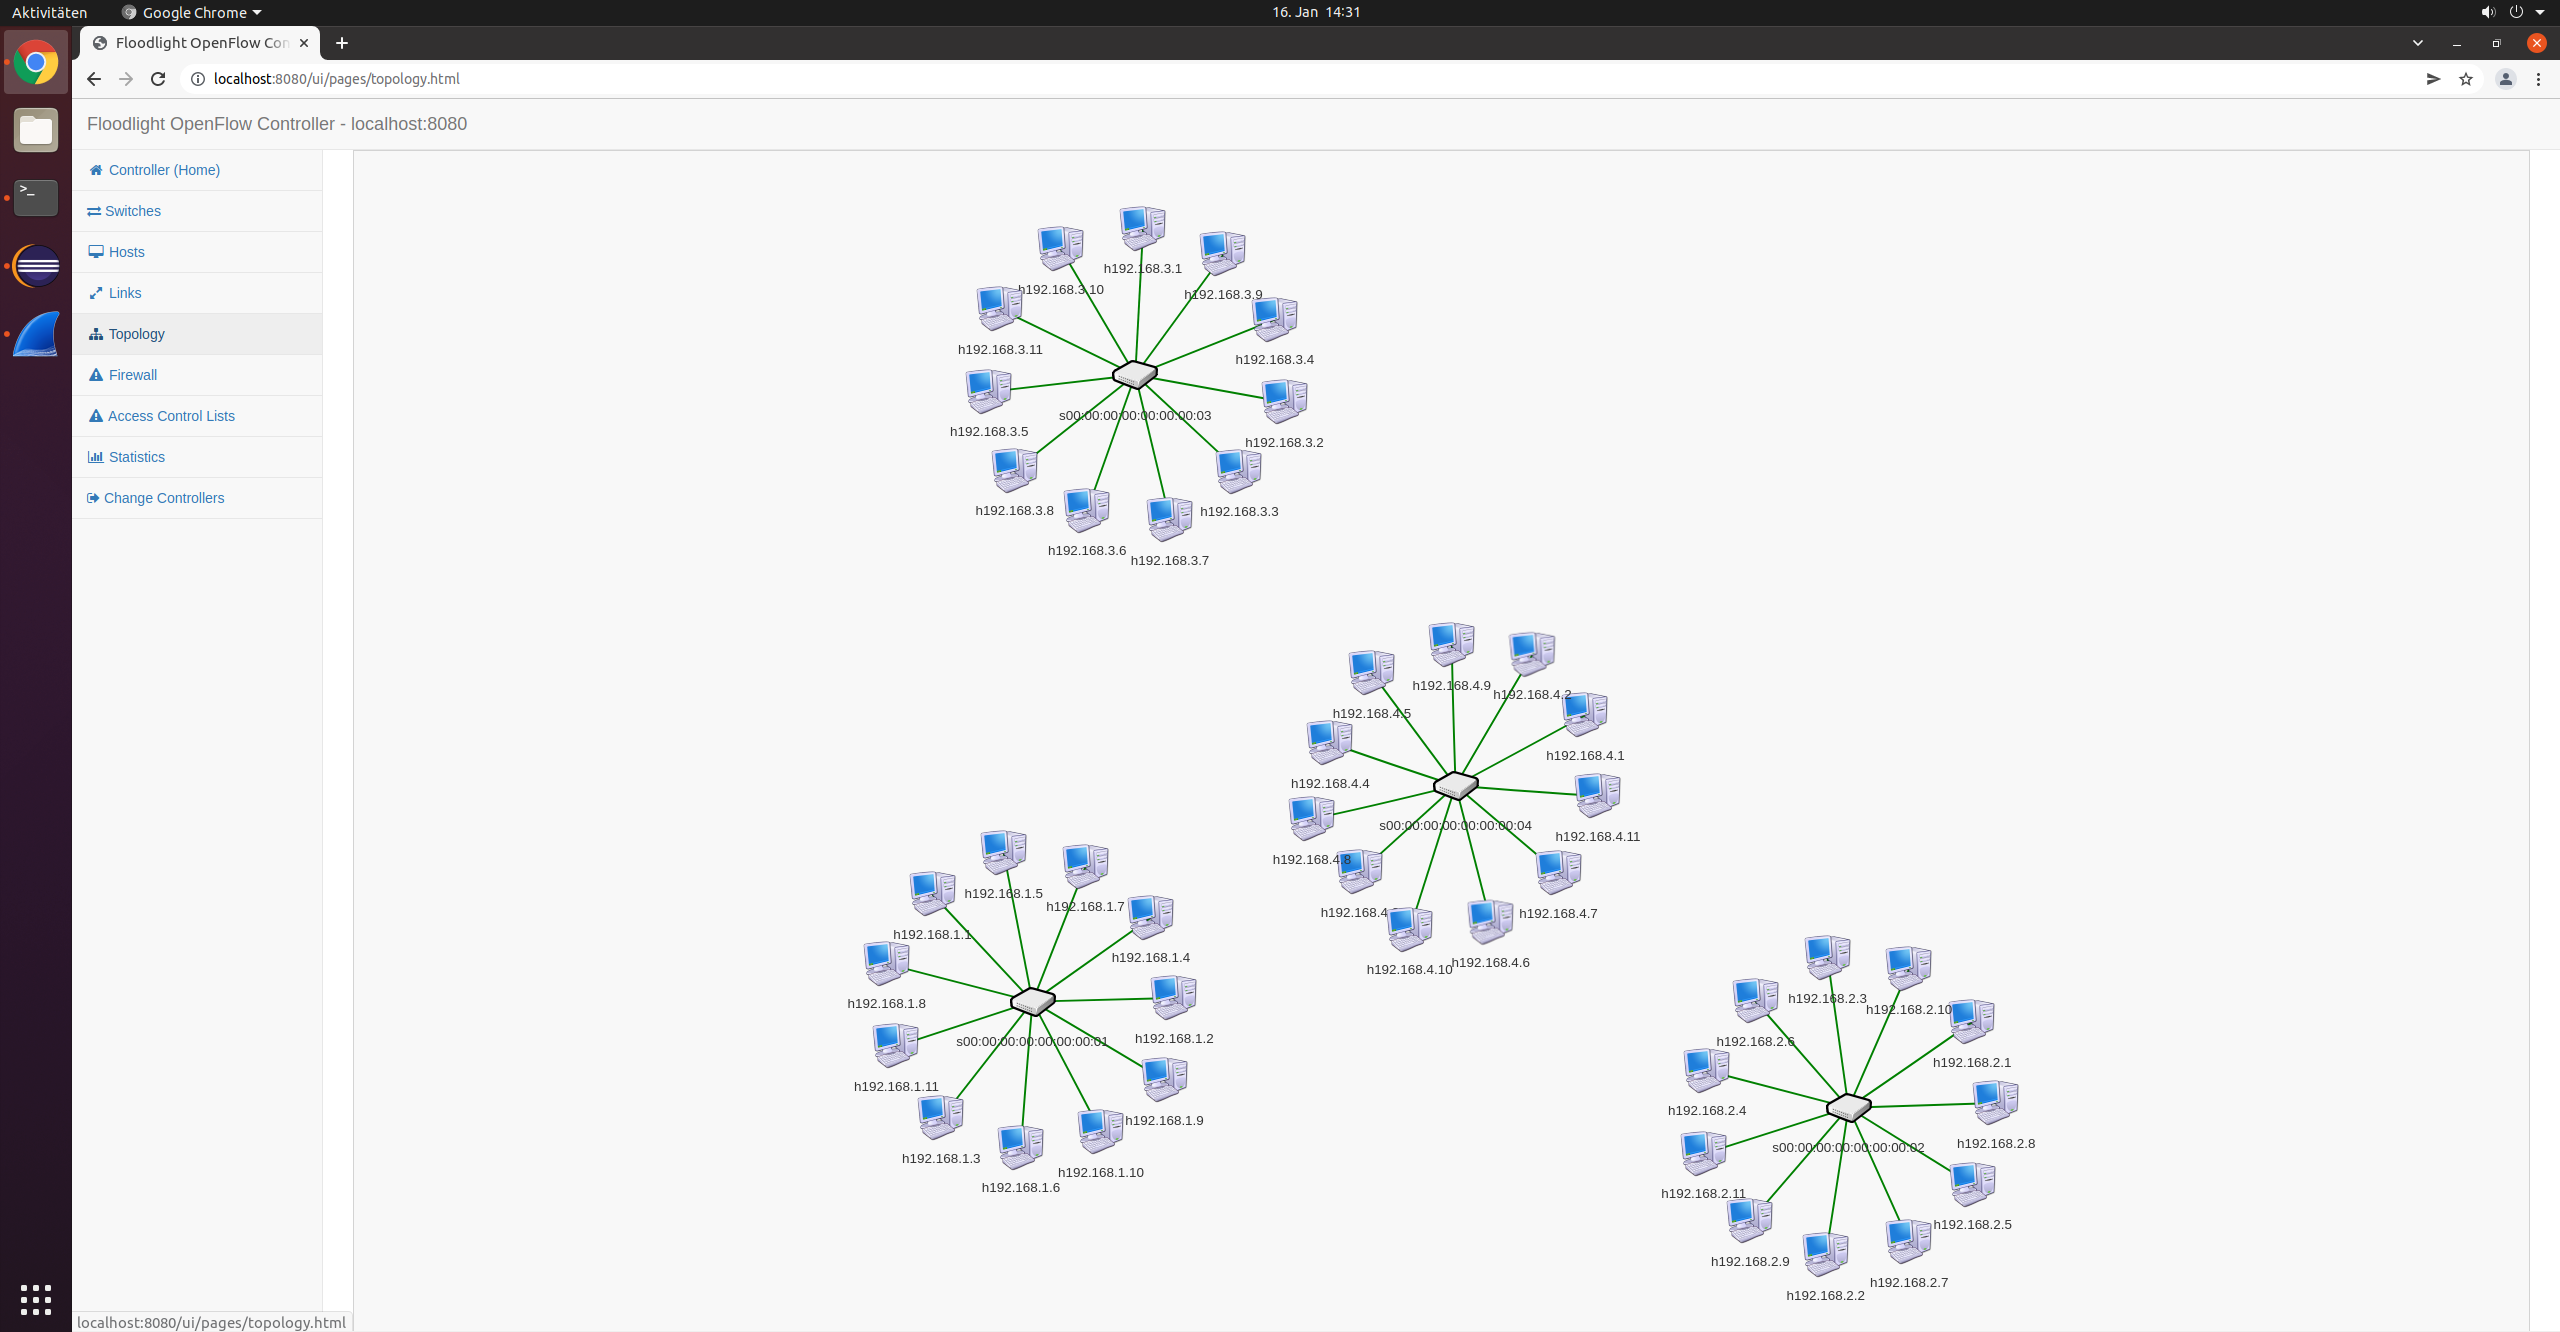
\includegraphics[width=1.0\textwidth]{Bilder/topo}
 \captionsetup{justification=centering}
 \caption{Topologie des Netzwerkes auf der Webbenutzeroberfläche von Floodlight}
 \label{topo}
\end{figure}


\subsection{Monitoring-Lösung}
{\tiny Verfasst von: Mücahit\par}
Für das zentrale Monitoring wird Nagios Core zum Einsatz kommen. Es kann auf einer großen Anzahl an Umgebungen installiert werden. Die Software bietet eine Weboberfläche, die von allen Netzwerkteilnehmern erreicht werden kann. Dabei kann die Verfügbarkeit, Geschwindigkeit und Dienste der Netzwerkkomponenten überprüft werden. Bei entstehenden Fehlern können Administratoren benachrichtigt werden, um die Fehler zu beheben. Bei großen Netzwerken spielt dies eine wichtige Rolle, da die Verfügbarkeit bei kritischen Anwendungen von großer Bedeutung ist.\par
Zunächst wird Nagios Core auf der VirtualBox-Maschine installiert, wo auch Mininet und Floodlight laufen. Bis jetzt lief Floodlight auf dem localhost, also der \textit{\textbf{127.0.0.1}} IP, welches nun geändert werden muss damit die Netzwerkteilnehmer auf die Floodlight REST-API und im Moment wichtiger auf den Nagios Core Dienst zugreifen können. Dafür werden im Mininet-Skript Befehle eingefügt, um den Switches 1-4 eine IP-Adresse zuzuweisen (siehe Abbildung \ref{switch}). Ebenfalls wird die Default-Route als \textit{\textbf{192.168.1.1}} hinzugefügt, da Nagios Core auf der IP \textit{\textbf{192.168.1.20}} laufen wird. Der Controller wurde auch konfiguriert auf dieser IP zu laufen. Nagios Core und der Controller sind nun von allen Netzwerkteilnehmern erreichbar.

\begin{figure}[H]
 \centering
 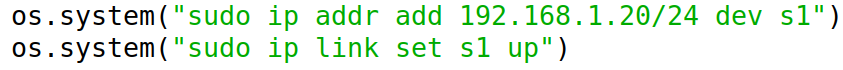
\includegraphics[width=0.7\textwidth]{Bilder/switch}
 \captionsetup{justification=centering, margin=2cm}
 \caption{Hinzufügen der Switch IP für s1}
 \label{switch}
\end{figure}
 
Die Installation von Nagios Core findet auf der Haupt-VirtualBox-Maschine statt und wird Schritt für Schritt erklärt. Die Befehle sollten nacheinander im Linux-Terminal ausgeführt werden.

\newlength\myboxwidth

\setlength{\myboxwidth}{\dimexpr\textwidth-2\fboxsep}

\begin{itemize}
\item[1.] Das Betriebssystem auf den neuesten Stand bringen
\end{itemize}
\colorbox{CadetBlue}{\textcolor{white}{\textbf{\textsf{\$ sudo apt update \& \& upgrade -y}}}}
\begin{itemize}
\item[2.] Alle benötigten Abhängigkeiten installieren
\end{itemize}
\colorbox{CadetBlue}{\parbox{\myboxwidth}{\textbf{\textsf{\textcolor{white}{\$ sudo apt install \hyp{}y build\hyp{}essential apache2 php openssl perl makephp\hyp{}gd libgd\hyp{}dev libapache2\hyp{}mod\hyp{}php libperl\hyp{}dev libssl\hyp{}dev daemonwget apache2\hyp{}utils unzip}}}}}
\begin{itemize}
\item[3.] Nagios Benutzer und Gruppe hinzufügen
\end{itemize}
\colorbox{CadetBlue}{\textcolor{white}{\textbf{\textsf{\$ sudo useradd nagios}}}}\\
\colorbox{CadetBlue}{\textcolor{white}{\textbf{\textsf{\$ sudo groupadd nagcmd}}}}\\
\colorbox{CadetBlue}{\textcolor{white}{\textbf{\textsf{\$ sudo usermod -a -G nagcmd nagios}}}}\\
\colorbox{CadetBlue}{\textcolor{white}{\textbf{\textsf{\$ sudo usermod -a -G nagcmd www-data}}}}
\begin{itemize}
\item[4.] Nagios in einen beliebigen Ordner herunterladen
\end{itemize}
\colorbox{CadetBlue}{\parbox{\myboxwidth}{\textbf{\textsf{\textcolor{white}{\$ wget https://assets.nagios.com/downloads/nagioscore/releases/nagios-4.4.5.tar.gz}}}}}
\begin{itemize}
\item[5.] Die Datei extrahieren und in den Ordner wechseln
\end{itemize}
\colorbox{CadetBlue}{\textcolor{white}{\textbf{\textsf{\$ tar -zxvf /tmp/nagios-4.4.5.tar.gz}}}}\\
\colorbox{CadetBlue}{\textcolor{white}{\textbf{\textsf{\$ cd /nagios-4.4.5/}}}}
\begin{itemize}
\item[6.] Nagios einstellen (hierbei wird der Benutzer und die Gruppe angegeben)
\end{itemize}
\colorbox{CadetBlue}{\parbox{\myboxwidth}{\textbf{\textsf{\textcolor{white}{\$ sudo ./configure --with-nagios-group=nagios--with-command-group=nagcmd --with-httpd\_conf=/etc/apache2/sites-enabled/}}}}}
\begin{itemize}
\item[7.] Die Dateien vorbereiten und installieren
\end{itemize}
\colorbox{CadetBlue}{\textcolor{white}{\textbf{\textsf{\$ sudo make all}}}}\\
\colorbox{CadetBlue}{\textcolor{white}{\textbf{\textsf{\$ sudo make install}}}}\\
\colorbox{CadetBlue}{\textcolor{white}{\textbf{\textsf{\$ sudo make install-init}}}}\\
\colorbox{CadetBlue}{\textcolor{white}{\textbf{\textsf{\$ sudo make install-config}}}}\\
\colorbox{CadetBlue}{\textcolor{white}{\textbf{\textsf{\$ sudo make install-commandmode}}}}
\begin{itemize}
\item[8.] Optional: Kontaktdaten in die contacts.cfg einfügen, um Notifications zu erhalten
\end{itemize}
\colorbox{CadetBlue}{\textcolor{white}{\textbf{\textsf{\$ sudo gedit /usr/local/nagios/etc/objects/contacts.cfg}}}}
\begin{itemize}
\item[9.] Webinterface installieren und Module aktivieren
\end{itemize}
\colorbox{CadetBlue}{\textcolor{white}{\textbf{\textsf{\$ sudo make install-webconf}}}}\\
\colorbox{CadetBlue}{\textcolor{white}{\textbf{\textsf{\$ sudo a2enmod cgi}}}}
\begin{itemize}
\item[10.] Nagios-Benutzer erstellen
\end{itemize}
\colorbox{CadetBlue}{\textcolor{white}{\textbf{\textsf{\$ sudo htpasswd -c /usr/local/nagios/etc/htpasswd.users nagiosadmin}}}}
\begin{itemize}
\item[11.] Webserver neustarten
\end{itemize}
\colorbox{CadetBlue}{\textcolor{white}{\textbf{\textsf{\$ sudo systemctl restart apache2}}}}
\begin{itemize}
\item[12.] Optional: Nagios Plugins herunterladen und installieren
\end{itemize}
\colorbox{CadetBlue}{\textcolor{white}{\textbf{\textsf{\$ wget https://nagios-plugins.org/download/nagios-plugins-2.3.3.tar.gz}}}}\\
\colorbox{CadetBlue}{\textcolor{white}{\textbf{\textsf{\$ tar -zxvf /tmp/nagios-plugins-2.3.3.tar.gz}}}}\\
\colorbox{CadetBlue}{\textcolor{white}{\textbf{\textsf{\$ cd /nagios-plugins-2.3.3/}}}}\\
\colorbox{CadetBlue}{\textcolor{white}{\textbf{\textsf{\$ sudo ./configure --with-nagios-user=nagios --with-nagios-group=nagios}}}}\\
\colorbox{CadetBlue}{\textcolor{white}{\textbf{\textsf{\$ sudo make}}}}\\
\colorbox{CadetBlue}{\textcolor{white}{\textbf{\textsf{\$ sudo make install}}}}
\begin{itemize}
\item[13.] Nagios bei Systemstart starten und Nagios ausführen
\end{itemize}
\colorbox{CadetBlue}{\textcolor{white}{\textbf{\textsf{\$ sudo systemctl enable nagios}}}}\\
\colorbox{CadetBlue}{\textcolor{white}{\textbf{\textsf{\$ sudo systemctl start nagios}}}}


Mit all den Schritten wurde Nagios Core inklusive der Plugins installiert. Der Webserver von Nagios läuft nach Neustarten des Dienstes auf den IP-Adressen der Switches. Dazu muss die IP inklusive des Pfades \textit{\textbf{/nagios}} aufgerufen werden. Dort sind im Moment nur Informationen über das System, welches Nagios ausführt, enthalten. Die Netzwerkkomponenten müssen manuell in Nagios eingefügt werden. Bevor das funktioniert, muss für die Switches eine Einstellung in der \textit{\textbf{nagios.cfg}} vorgenommen werden. Dort muss die Raute vor dem \textit{\textbf{cfg\_file=/usr/local/nagios/etc/objects/switch.cfg}} Befehl entfernt werden, damit die \textit{\textbf{switch.cfg}} in Nagios mitübernommen wird. Nun werden in der \textit{\textbf{switch.cfg}} alle Switches mit der Bezeichnung, deren IP und der zugehörigen Gruppe aufgelistet (siehe Abbildung \ref{nagios-switch}). Danach können sogenannte Services für die Überwachung der Verfügbarkeit, der Geschwindigkeit und weitere Informationen hinzugefügt werden (siehe Abbildung \ref{nagios-service}). Anschließend muss der Nagios Dienst neu gestartet werden. Um Fehler zu vermeiden, sollte per \textit{\textbf{sudo /usr/local/nagios/bin/nagios -v /usr/local/nagios/etc/nagios.cfg}} Befehl geschaut werden, ob Unstimmigkeiten bei den geänderten Konfigurationen existieren.\par

\begin{figure}[H]
 \centering
 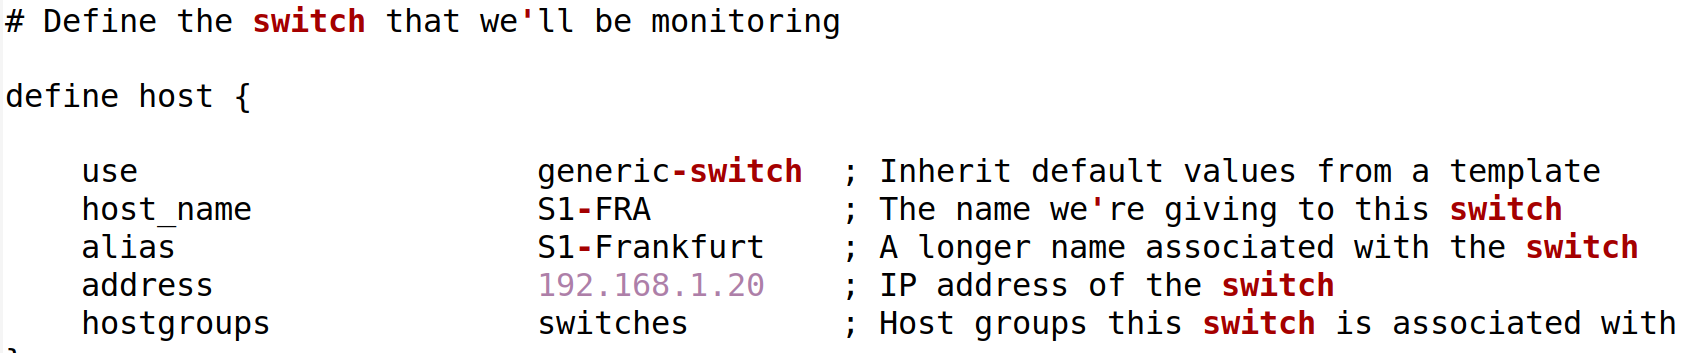
\includegraphics[width=1.0\textwidth]{Bilder/nagios-switch}
 \captionsetup{justification=centering, margin=2cm}
 \caption{Definition der Switch für Nagios}
 \label{nagios-switch}
\end{figure}

\begin{figure}[H]
 \centering
 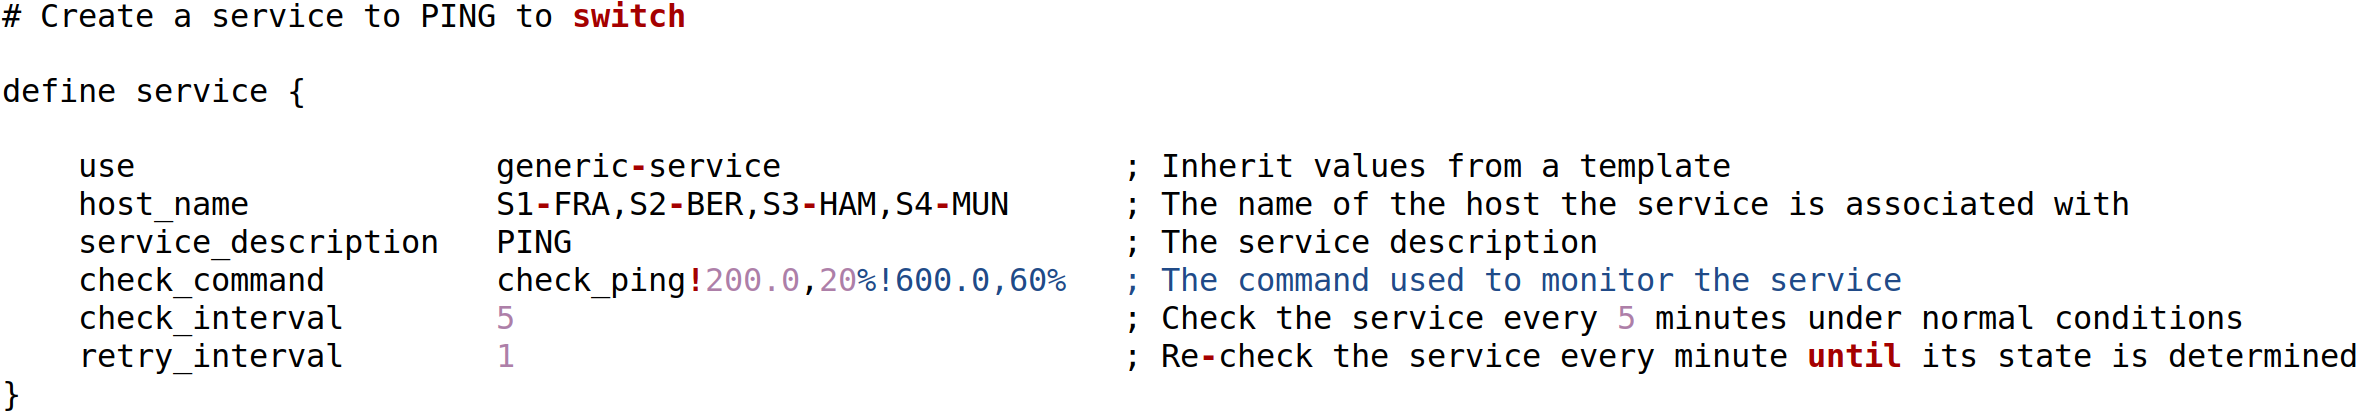
\includegraphics[width=1.0\textwidth]{Bilder/nagios-service}
 \captionsetup{justification=centering, margin=2cm}
 \caption{Definition der Services für die Switch}
 \label{nagios-service}
\end{figure}
Nachdem alle Netzwerkteilnehmer und -komponenten hinzugefügt und die gewünschten Services eingestellt worden sind, werden alle Informationen auf der Webbenutzeroberfläche angezeigt (siehe Abbildung \ref{nagios}). Unter dem Reiter Hosts kann die Verfügbarkeit aller Teilnehmer angezeigt werden. Die Verfügbarkeit kann unter mehreren Zuständen unterscheiden. Ein Host kann daher den Zustand \textit{\textbf{Up, Down, Unreachable}} und \textit{\textbf{Pending}} haben, welche auch mit Farben visualisiert werden. Unter Services werden alle Teilnehmer mit den konfigurierten Services angezeigt. Die Services haben ebenfalls Zustände. Dazu gehört unteranderem \textit{\textbf{Ok, Warning, Unknown, Critical}} und \textit{\textbf{Pending}}, die ebenfalls mit Farben visualisiert werden. Bei Host Groups werden die Teilnehmer gruppiert und die Informationen zusammengefasst angezeigt. Des Weiteren können viele weitere Einstellungen bezüglich der Benachrichtigungen und der Services über die Webbenutzeroberfläche vorgenommen werden. Dazu klickt man auf einen Teilnehmer und kann auf dem rechten Abschnitt sogenannte \textit{\textbf{Host Commands}} benutzen. Beispielsweise können Kommentare zu Hosts oder Services verfasst werden, damit andere Nutzer bestimmte Vorgänge nachvollziehen können. Zusammenfassend kann über Nagios das gesamte Netzwerk zentral überwacht werden.


\begin{figure}[H]
 \centering
 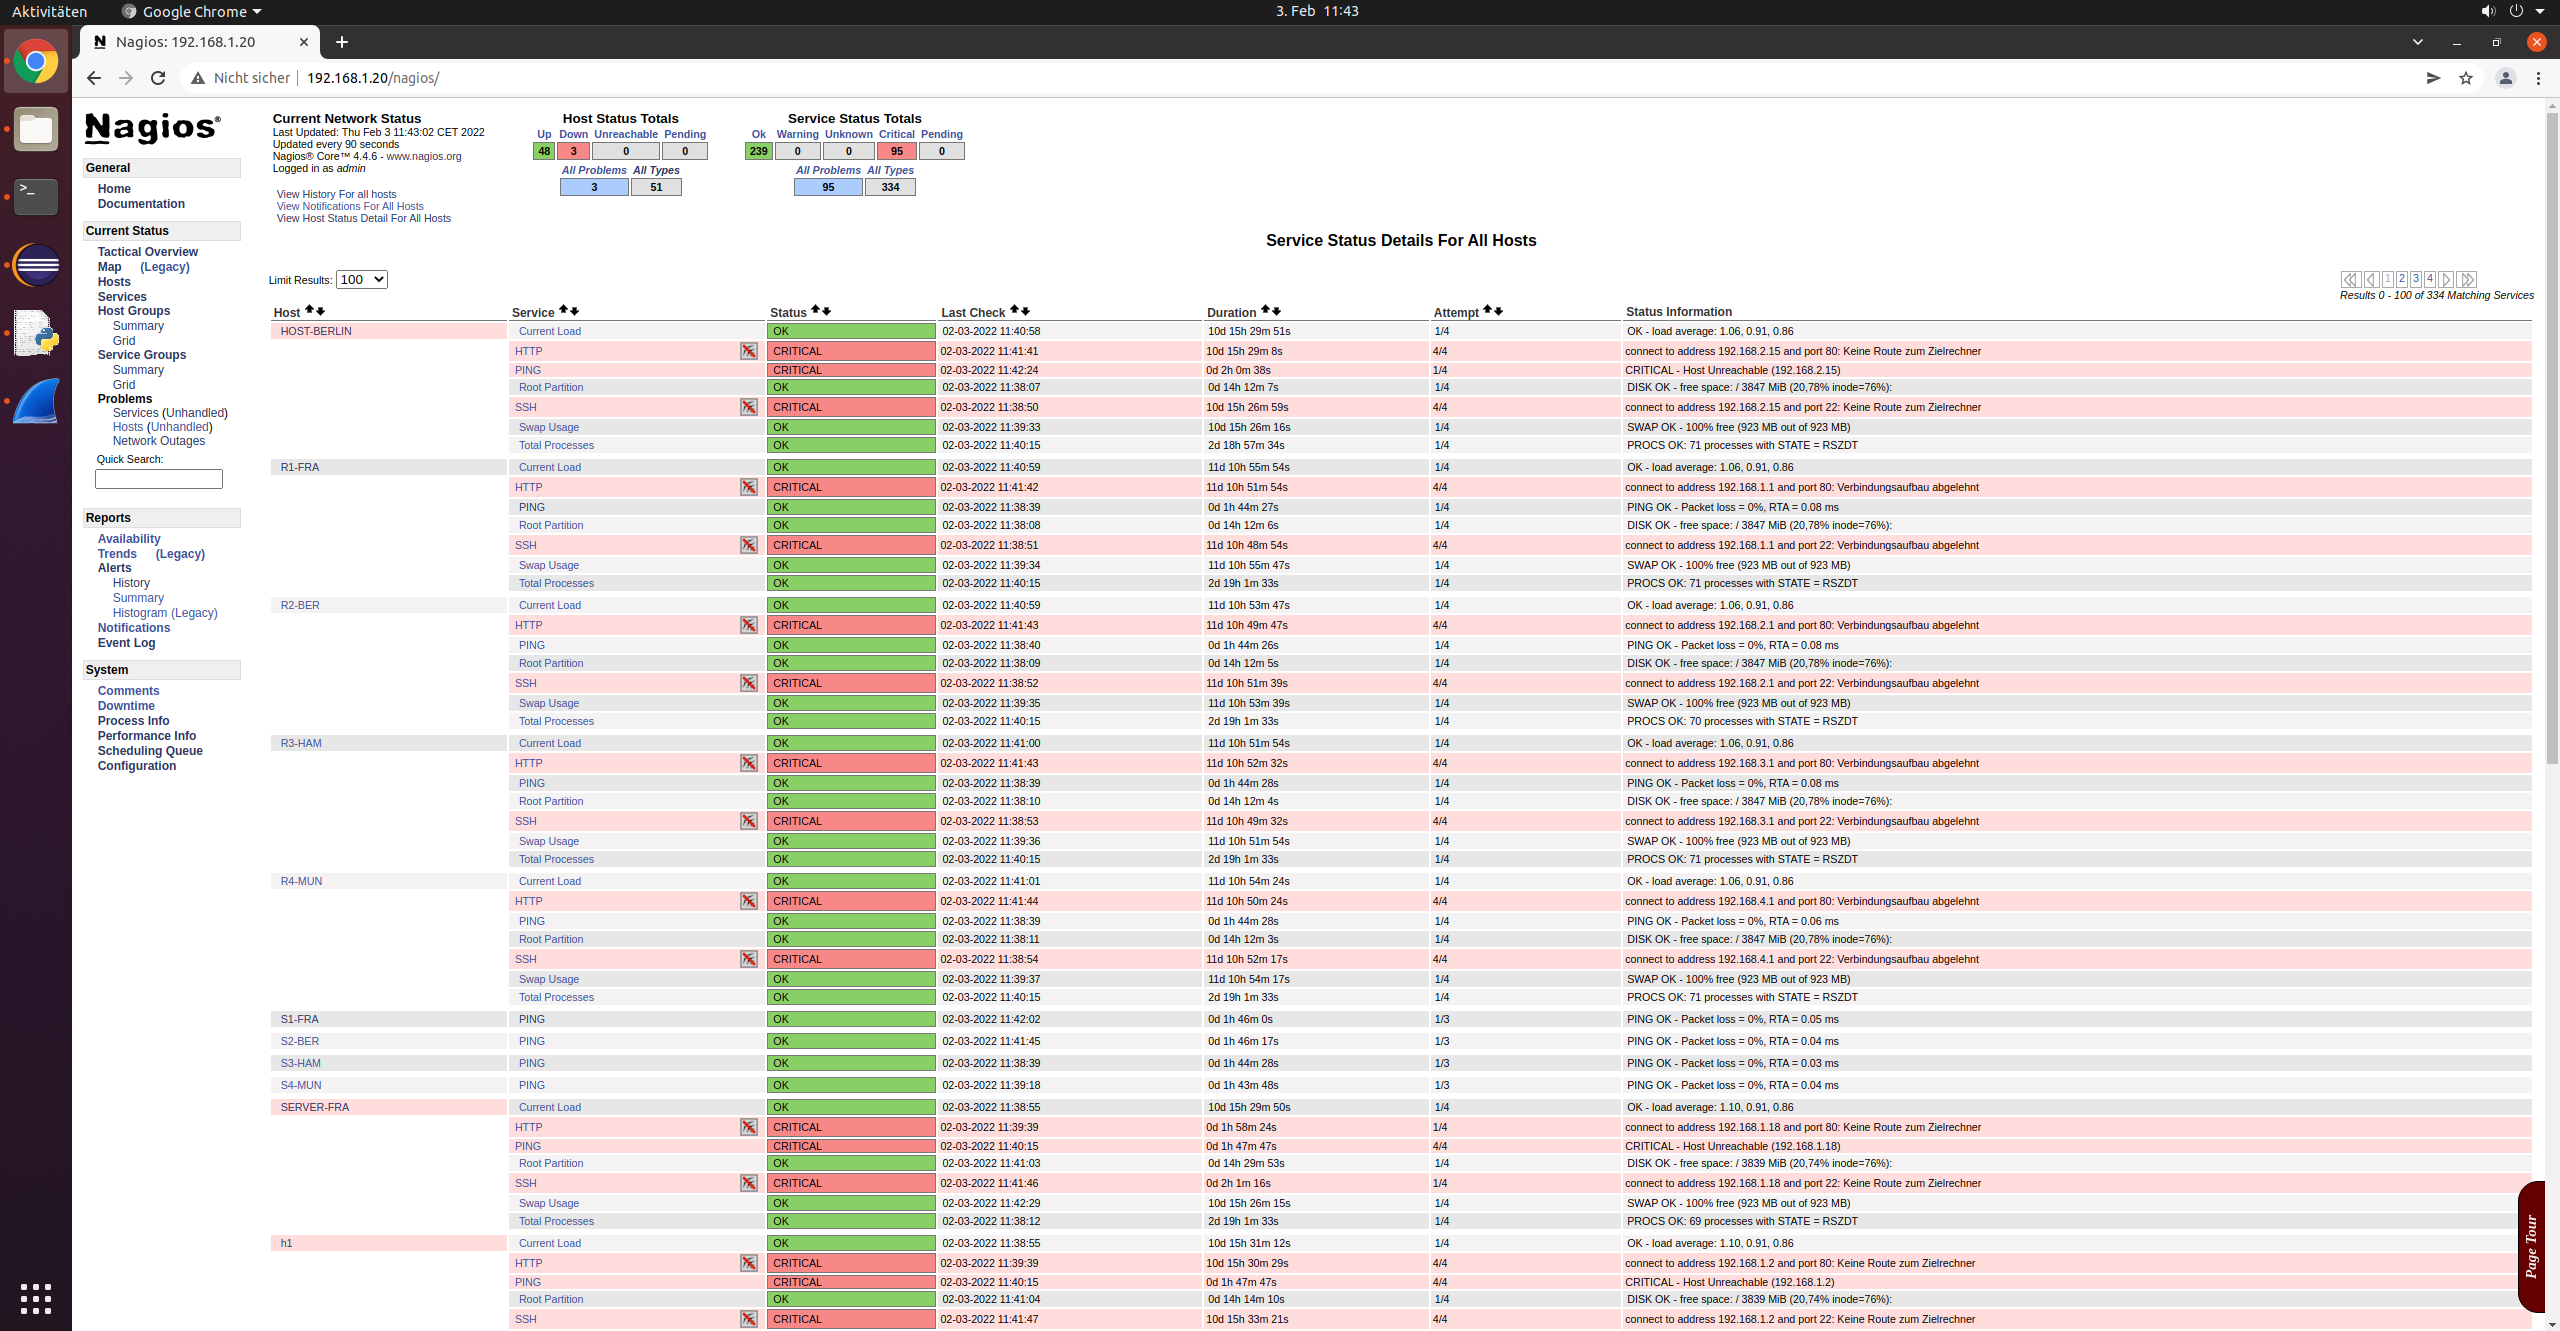
\includegraphics[width=1.0\textwidth]{Bilder/nagios}
 \captionsetup{justification=centering, margin=2cm}
 \caption{Webbenutzeroberfläche von Nagios Core}
 \label{nagios}
\end{figure}


\section{Realisierung einer Quality of Service Funktion}
{\tiny Verfasst von: Mücahit\par}
Die Quality of Service Funktion gewährleistet die Fähigkeit des Netzwerkes, Anwendungen und Datenverkehr selbst bei begrenzter Netzwerkkapazität zuverlässig mit hoher Priorität auszuführen. Das Netzwerkes muss für alle Audio- und Video-Konferenzen innerhalb der Lokationen genügend Bandbreite zur Verfügung stellen. Die Verbindung zwischen den Lokationen besteht aus einer Standleitung mit einer Geschwindigkeit von 20 Megabit.

\subsection{Vorüberlegung}
{\tiny Verfasst von: Mücahit\par}
Pakete, die für die Audio- und Videokonferenzen verantwortlich sind, müssen an dem Switch über den Controller priorisiert werden. Durch die Priorisierung sollen bei einer Auslastung des Netzwerkes die Audio- und Videokonferenzen stabil und flüssig laufen. Nach einer ausgiebigen Recherche kam der Entschluss, UDP Pakete zu priorisieren, da die meisten Videokonferenzprogramme wie beispielsweise Skype und Zoom diese verwenden. Zusätzlich muss getestet werden, wie viel Megabit pro Host eine ausreichende Bandbreite darstellen.\par
An dem Port der Switch, der zum Router der Lokationen führt, werden zwei sogenannte Queues erstellt. Eine Queue wird für die Audio- und Videokonferenzen und die andere Queue für den restlichen Datenverkehr verwendet. Dabei erhalten die Queues Eigenschaften wie der minimalen und/oder maximalen Bandbreite zur Gewährleistung der Quality of Service. Nach der Konfiguration sollte gezeigt werden, ob Pakete tatsächlich über die Queue verlaufen. 

\subsection{Durchführung}
{\tiny Verfasst von: Mücahit\par}
Auf allen vier Switches wird zuerst der Befehl \textit{\textbf{sudo ovs\hyp{}vsctl set port Router\hyp{}Port qos=@newqos \hyp{}\hyp{} \hyp{}\hyp{}id=@newqos create qos type=linux\hyp{}htb other\hyp{}config:max\hyp{}rate=20000000 queues:0=@newqueue0 queues:1=@newqueue1 \hyp{}\hyp{} \hyp{}\hyp{}id=@newqueue0 create queue other\hyp{}config:max\hyp{}rate=20000000 \hyp{}\hyp{} \hyp{}\hyp{}id=\linebreak{}@newqueue1 create queue other\hyp{}config:min\hyp{}rate=7000000 other\hyp{}config:max\hyp{}rate=20000000}} mit der Angabe der Bezeichnung für den Port zum Router ausgeführt. Das Ganze geschieht im Ubuntu\hyp{}Terminal während Mininet ausgeführt wird. Dabei wird auf dem Switch die Quality of Service und genau zwei Queues konfiguriert, die sich anhand der ID unterscheiden. Die allgemeine Bandbreite des Ports wird auf \textit{\textbf{20 Megabit}}, die \textit{\textbf{Queue 0}} auf \textit{\textbf{maximal 20 Megabit}} und die \textit{\textbf{Queue 1}} auf \textit{\textbf{minimal sieben}} und \textit{\textbf{maximal 20 Megabit}} gesetzt. Die minimale Bandbreite für die Priorisierung wurde anhand eines Selbst\hyp{}Tests mit Zoom und der Information des Ressourcenmonitors von Windows festgelegt. Dabei wurde mit Video\hyp{} und Audioübertragungen eine Uploadrate zwischen \textit{\textbf{500\hyp{}900 Kilobit}} pro Sekunde gemessen. Daraus resultierend wurden für zehn Arbeitsplätzen die Geschwindigkeit auf Minimum sieben Megabit eingestellt.\par
Der Datenverkehr wird über den Open vSwitch konfiguriert. Der Verkehr soll entweder auf die \textit{\textbf{Queue 0}} oder \textit{\textbf{Queue 1}} weitergeleitet werden. So erhaltet der Verkehr die Eigenschaften dieser Queue bezüglicher der festgelegten Raten. Dazu wird über das Mininet-Skript im Ubuntu-Terminal für alle Switches der Befehl \textit{\textbf{sudo ovs-ofctl add-flow Switch-Bezeichnung priority=1000, actions=set\_queue:0, normal}} ausgeführt. Der Befehl leitet jedes Paket an die Queue 0. Somit wäre jeglicher Datenverkehr auf maximal 20 Megabit begrenzt. Als Nächstes werden nur die UDP-Pakete mit dem angegebenen Adressenbereich mit dem Befehl \textit{\textbf{sudo ovs-ofctl add-flow Switch-Bezeichnung priority=65535, udp, nw\_src=192.168.0.0/16, nw\_dst=192.168.0.0/16, actions=set\_queue:1, normal}} bei allen Switches auf die Queue 1 weitergeleitet. Damit hätten die UDP-Pakete eine minimale Bandbreite von sieben und eine maximale Bandbreite von 20 Megabit. Bei den Bedingungen wurde zusätzlich die Priorität eingegeben. Desto höher die Priorität gesetzt wird, desto höher ist die Priorität des Flows und auch somit die Wichtigkeit. Bei der Bedingung für die Quality of Service wird die Priorität auf das Maximum, nämlich \textit{\textbf{65535}}, gestellt. Beim restlichen Datenverkehr kann dieser beliebig größer null gewählt werden. Zusätzlich wird am Ende jeder Bedingung der Flow auf normal gesetzt. Dieser bedeutet, dass das Paket wie gewöhnlich im Layer zwei weiterverarbeitet wird.

\subsection{Ergebnis}
{\tiny Verfasst von: Mücahit\par}
Die Quality of Service und Queue Einstellungen können über die Befehle \textit{\textbf{sudo ovs-vsctl list qos}} und \textit{\textbf{sudo ovs-vsctl list queue}} angezeigt werden (siehe Abbildung \ref{queue-qos}). Mit dem Befehl \textit{\textbf{sudo ovs-ofctl dump-flows switchbezeichnung}} können die Flows des jeweiligen Switches ausgegeben werden. Dort werden unteranderem die Flows für die Quality of Service und des restlichen Datenverkehrs angezeigt.

\begin{figure}[H]
 \centering
 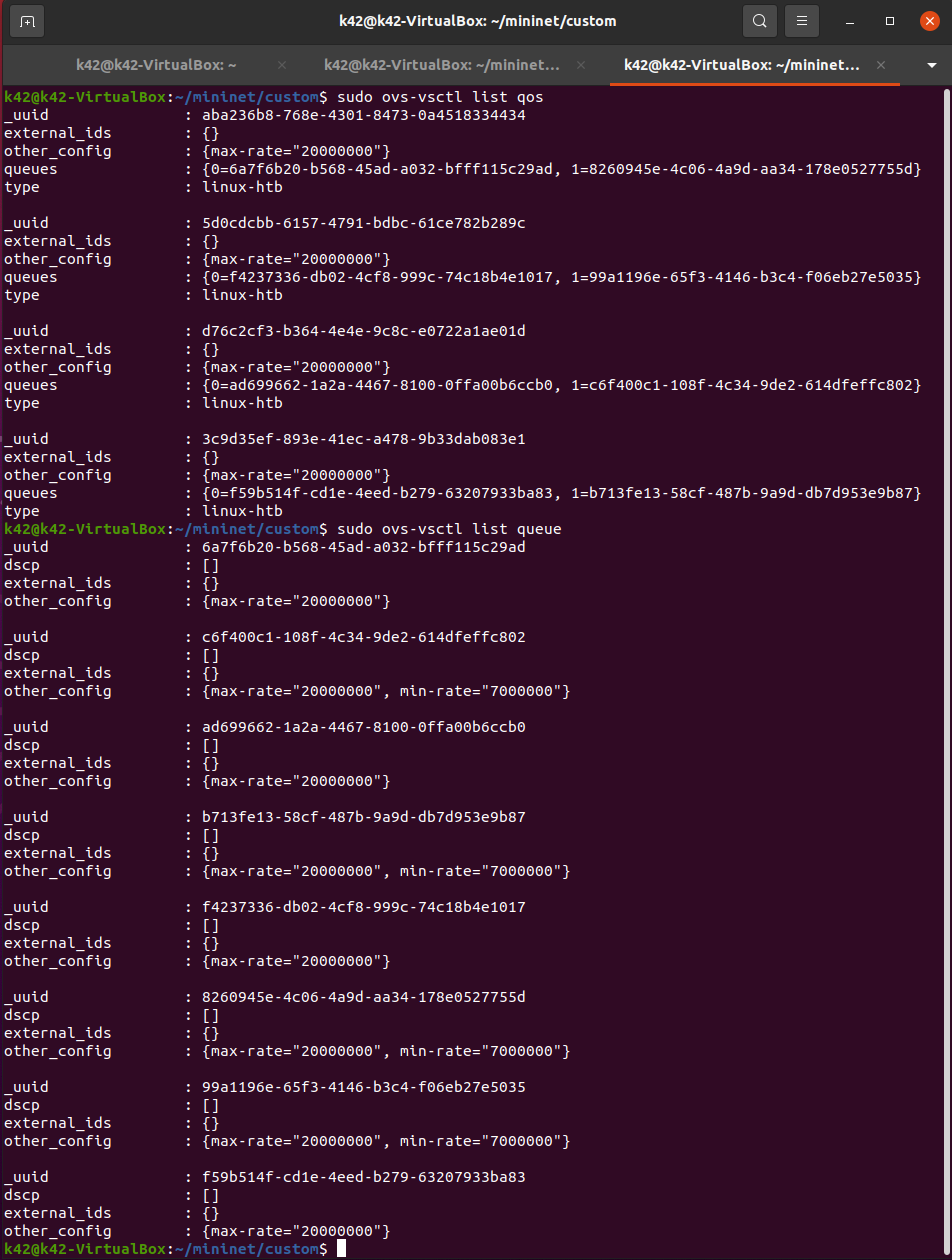
\includegraphics[width=0.7\textwidth]{Bilder/queue-qos}
 \captionsetup{justification=centering}
 \caption{Ausgabe der QoS und Queue der Switches aller Lokationen}
 \label{queue-qos}
\end{figure}

Für den Test wurden zwei weitere VirtualBox-Maschinen mit Ubuntu aufgestellt. Eine Maschine stellt den Server in der Lokation Frankfurt dar. Die andere Maschine stellt einen Host in der Berliner Lokation dar. Beide Maschinen wurden mit der Haupt-VirtualBox-Maschine über eine interne Schnittstelle verbunden. Der Frankfurter Server besitzt die IP \textit{\textbf{192.168.1.18}}, während der Berliner Host die IP \textit{\textbf{192.168.2.15}} besitzt. Dies wurde per Netplan eingerichtet, welcher per \textit{\textbf{sudo apt install netplan.io}} Befehl auf beiden Systemen installiert worden ist. Danach wurden in den Konfigurationsdateien im Dateipfad \textit{\textbf{/etc/netplan/}} die dementsprechende IP-Adresse, das Gateway der Lokation eingegeben und dhcp auf false gestellt. Anschließend wurden die Einstellungen mit dem Befehl \textit{\textbf{sudo netplan apply}} übernommen. Nach den Schritten besteht zwischen dem Host in Berlin und dem Server in Frankfurt über die Haupt-VirtualBox-Maschine eine Verbindung.\par
Um nun die Quality of Service und Queue Konfiguration zu testen, wurde auf dem Server in Frankfurt der Prosody \textit{\textbf{Extensible Messaging and Presence Protocol}} (XMPP) Server installiert und konfiguriert. Dazu wurde der Befehl \textit{\textbf{sudo apt-get install prosody}} im Terminal eingegeben. Anschließend wurde der Server anhand der Datei im Pfad \textit{\textbf{/etc/prosody/prosody.cfg.lua}} konfiguriert und mit dem Befehl \textit{\textbf{sudo systemctl restart prosody-service}} neu gestartet. Nun läuft in der Frankfurter Lokation ein XMPP-Server. Des Weiteren wurde auf dem Server in Frankfurt und auf dem Host in Berlin der XMPP-Client Pidgin mit dem Befehl \textit{\textbf{sudo apt install pidgin}} installiert. Es wurde danach über Prosody zwei XMPP-Benutzer mit dem Befehl \textit{\textbf{sudo prosodyctl adduser user1@192.168.1.18}} und \textit{\textbf{sudo prosodyctl adduser user2@192.168.1.18}} mit der Eingabe eines Passwortes erstellt. Mit dem Pidgin-Client wurden in beiden Lokationen die Nutzer eingeloggt, die sich zusätzlich gegenseitig zu den Kontakten hinzugefügt haben. Nun waren die Nutzer gegenseitig für einander sichtbar. Jetzt kann per Rechtsklick ein Sprachanruf gestartet und getätigt werden (siehe Abbildung \ref{pidgin}). Während dem Anruf kann per \textit{\textbf{sudo ovs-ofctl dump-flows s1}} Befehl erkannt werden, dass die Anzahl der Pakete für die vorher eingefügte UDP-Bedingung stetig steigen (siehe Abbildung \ref{udp}). Per Wireshark können die zwischen den Standorten Übermittelten UDP-Pakete betrachtet werden (siehe Abbildung \ref{udp2}). Damit wurde gezeigt, dass die UPD-Pakete des Sprachanrufes über die gesetzte Bedingung auf die Queue 1 weitergeleitet wird. Somit erhalten alle Pakete eine minimale Geschwindigkeit von sieben Megabit.

\begin{figure}[H]
 \centering
 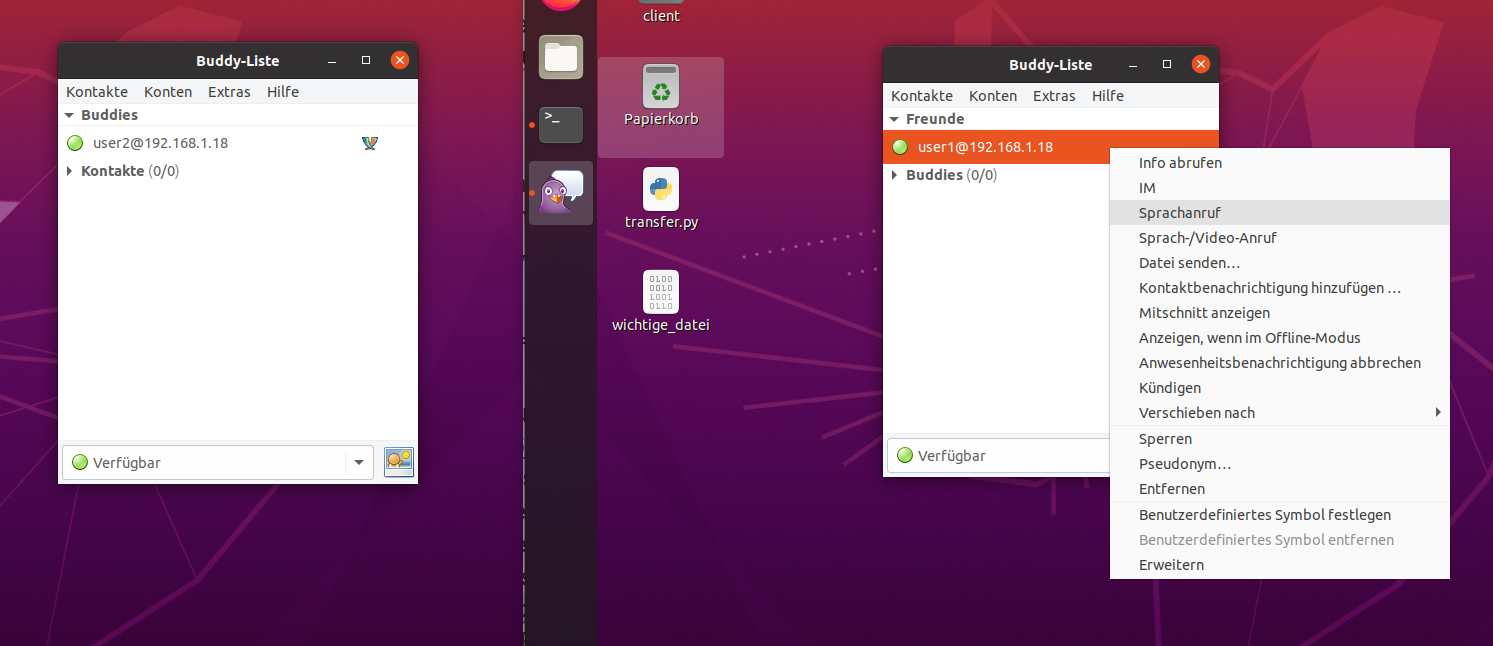
\includegraphics[width=0.8\textwidth]{Bilder/pidgin}
 \captionsetup{justification=centering}
 \caption{Sprachanruf zwischen Berlin und Frankfurt}
 \label{pidgin}
\end{figure}

\begin{figure}[H]
 \centering
 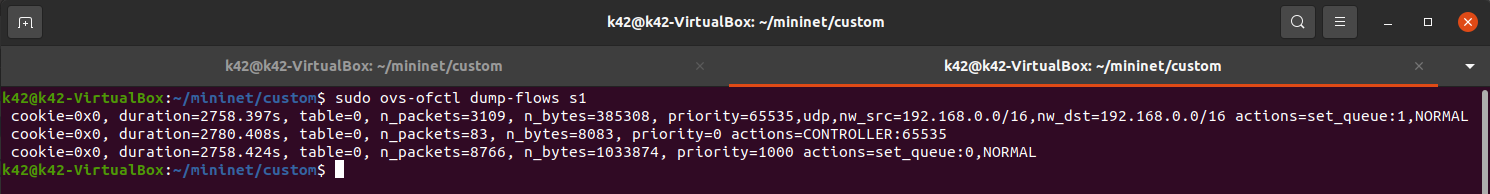
\includegraphics[width=0.8\textwidth]{Bilder/udp}
 \captionsetup{justification=centering}
 \caption{Ausgabe der Flows von s1}
 \label{udp}
\end{figure}

\begin{figure}[H]
 \centering
 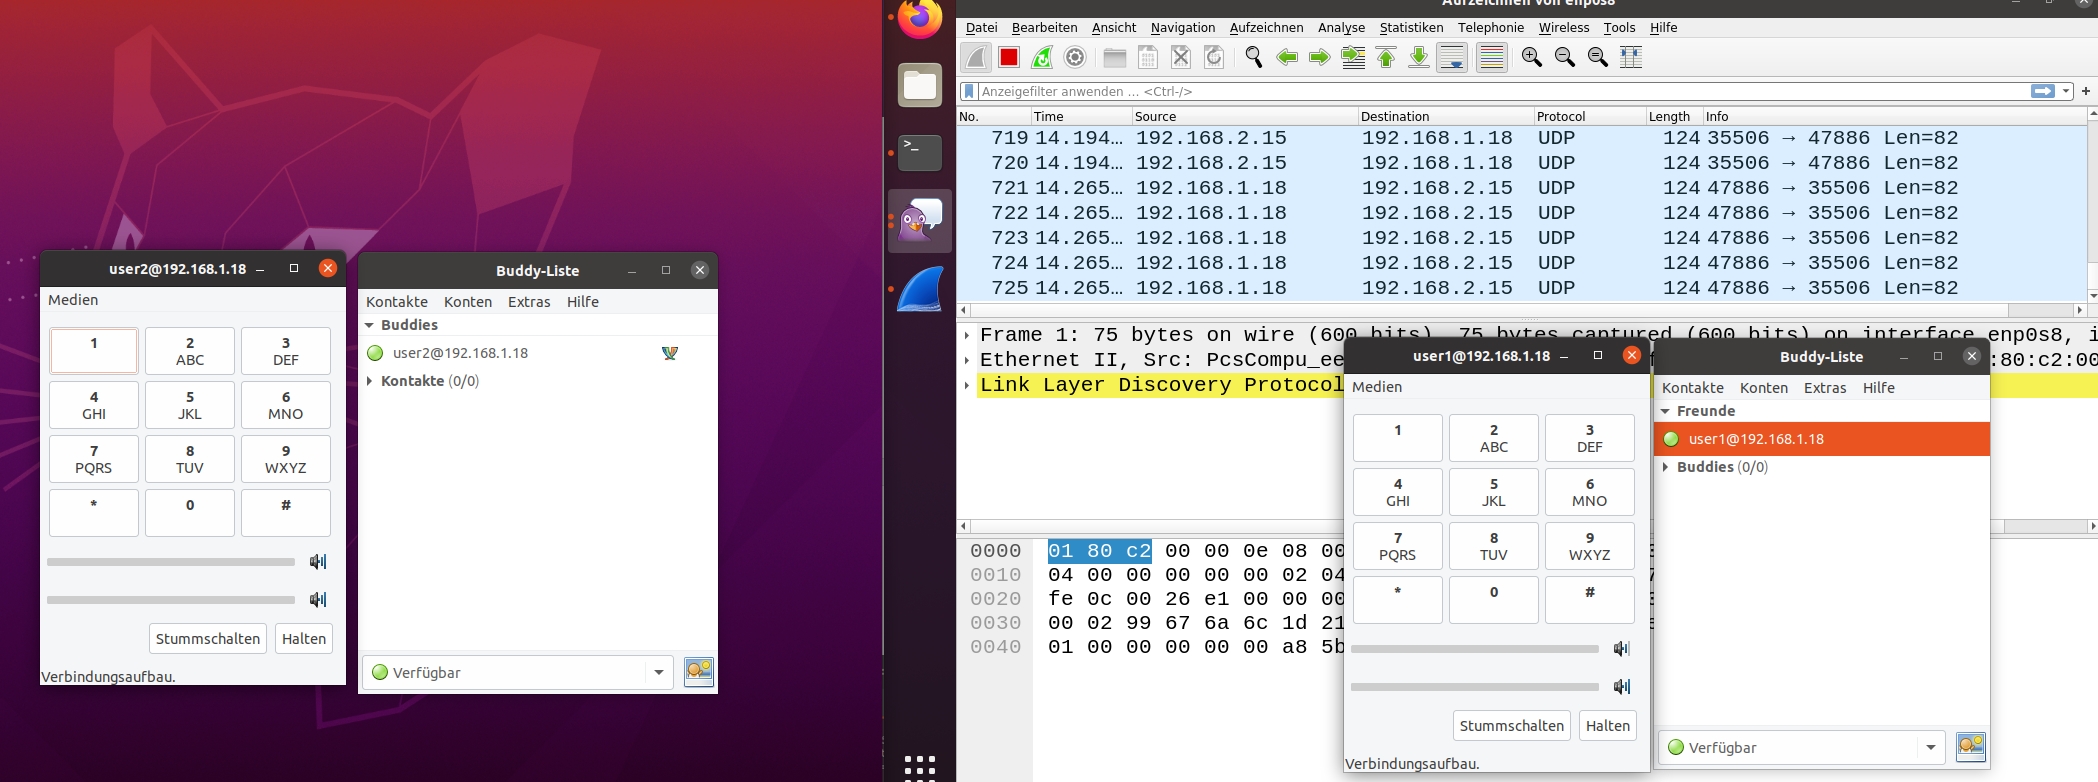
\includegraphics[width=0.8\textwidth]{Bilder/udp2}
 \captionsetup{justification=centering}
 \caption{UDP-Pakete während dem Sprachanruf}
 \label{udp2}
\end{figure}

\section{Priorisierung der Datenübertragung über API}
\subsection{Vorüberlegung}
{\tiny Verfasst von: Mücahit\par}
Anhand des Schlüsselwortes \textit{\textbf{priority}} soll der Flow einer Datenübertragung zwischen der Lokation Berlin und Frankfurt priorisiert werden. Allen anderen Flows werden auf der Strecke eine geringere Priorität zugewiesen, sodass die Datenübertragung bevorzugt wird. Falls die gleiche Priorität bei zwei Flows existiert, wird der Flow mit der genaueren Bedingung verwendet. Die Datenübertragung soll über einem in der Zentrale eingerichteten \textit{\textbf{Secure-Shell}} (SSH) Server laufen. Dazu wird auf dem Host in Berlin ein \textit{\textbf{SSH-Client}} benötigt. Bei der Übertragung nutzt SSH üblicherweise den \textit{\textbf{Port 22}} über dem \textit{\textbf{Transport Control Protocol}} (TCP). Mit dieser Information wird die Bedingung für die Priorisierung des Flows festgelegt. Die Übertragung und die Priorisierung werden versucht, in einem ausführbaren Python-Skript zu realisieren, bei der die Angabe der IPv4-Adresse des Hosts in Berlin und des Hosts in der Zentrale als Parameter nötig werden. Es könnte die IPv4-Adresse der Quelle und des Ziels auch automatisch vom Skript durch das System ermittelt werden. Das Skript sollte folgende Schritte beinhalten:
\begin{itemize}
\item[1.] IP-Quelle und Ziel eingeben und einlesen (später -> automatisieren)
\item[2.] Voraussichtlichen Flow über API priorisieren. Restlichen Datenverkehr drosseln
\item[3.] Übertragung per SSH starten
\item[4.] Bei Erfolg Priorisierung und Drosslung wieder aufheben
\item[5.] Bei Fehler Fehlermeldung ausgeben
\end{itemize}
Der Controller, genauer der OpenFlow-Server und der Restserver laufen unter der IP-Adresse \textit{\textbf{192.168.1.20}} und kann von jedem Host erreicht werden. Dies ist wichtig, da die Priorisierung von außen durchgeführt wird. Ansonsten kann der Controller, wenn dieser auf \textit{\textbf{localhost}} läuft, nicht erreicht werden.


\subsection{Durchführung}
{\tiny Verfasst von: Mücahit\par}
\begin{wrapfigure}{R}{0.5\textwidth}
	\vspace{-\baselineskip}
 	\centering
 	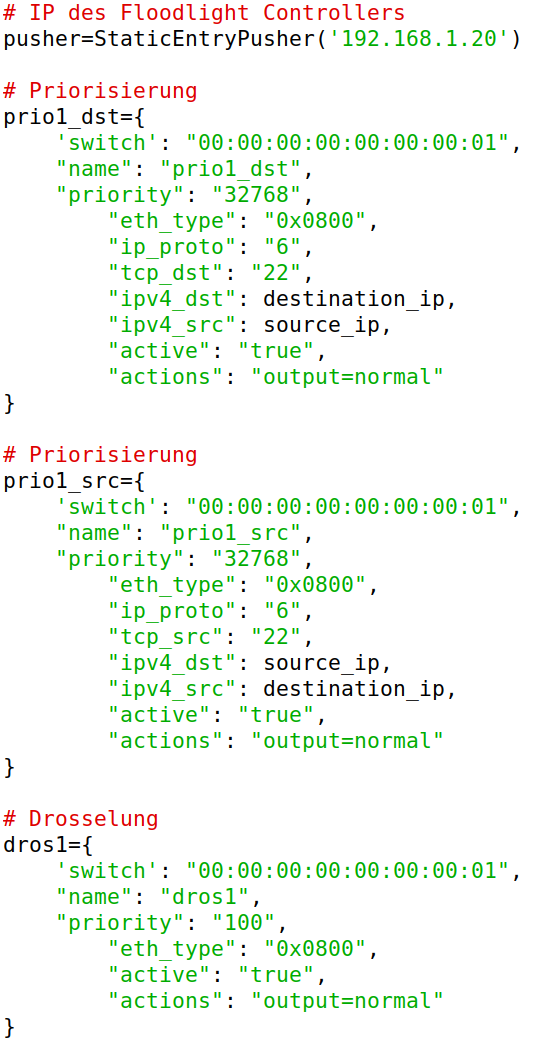
\includegraphics[width=0.35\textwidth]{Bilder/transfer-flow}
 	\caption{Flows für die Priorisierung und die Drosselung}
 	\label{transfer-flow}
\end{wrapfigure}
Die Durchführung erfolgt mit den im vorherigen Kapitel aufgestellten VirtualBox Maschinen. Auf dem Server in Frankfurt wurde per \textit{\textbf{sudo apt install openssh-server}} Befehl der SSH-Server installiert. Dieser wurde eingestellt, auf der IP des Servers zu laufen. Dafür wurde per \textit{\textbf{sudo nano /etc/ssh/sshd\_config}} Befehl in der Konfigurationsdatei des SSH-Servers die IP-Adresse geändert und die Publickeyauthentication ausgeschaltet. Anschließend wurde der SSH-Server-Dienst mit dem Befehl \textit{\textbf{sudo systemctl restart ssh}} neugestartet, um die Einstellungen zu übernehmen. Auf dem Berliner Host wurde per \textit{\textbf{dd if=/dev/zero of=wichtige\_datei bs=50MB count=1}} Befehl eine Dummy-Datei für die Übertragung auf dem Schreibtisch erstellt.\par

Der Server betreibt einen SSH-Server und der Host einen SSH-Client, womit wichtige Dateien übertragen werden. Dafür wurde auf dem Host ein Python-Skript erstellt, welcher näher erläutert wird. Vorher muss per \textit{\textbf{sudo pip install paramiko scp}} Befehl die benötigten Python-Module für die SSH-Verbindung installiert werden. Die Installation geschieht mit pip dem Paketverwaltungsprogramm von Python. Das Skript holt sich automatisch die IP-Adresse des Senders anhand der \textit{\textbf{get\_IP-Methode}} und speichert diese in eine Variable. Anschließend wird die Angabe der Informationen zur Übermittlung verlangt. Dazu gehört der Dateipfad, die IP-Adresse des Empfängers, den Servernamen, das Serverpasswort und den Pfad, wohin die Datei im Ziel gespeichert werden soll (siehe Abbildung \ref{transfer-daten}). Danach wird ein Objekt als Rest-Client zur Übermittlung der Prioritätensetzung erstellt. Dieser bekommt die \textit{\textbf{192.168.1.20}} als IP-Adresse des Controllers gesetzt. Jetzt werden die Flows zur Priorisierung erstellt. Dabei werden jeweils drei gleiche Flows auf den Switch in der Berliner Lokation mit der ID 2 und auf den Switch in der Frankfurter Lokation mit der ID 1 zugewiesen. Die zwei Flows priorisieren TCP-Pakete mit dem Port 22 und der angegebenen Quell- und Zieladresse. Beide Flows decken eingehende und ausgehende Pakete ab und bekommen \textit{\textbf{32768}} als die maximale Priorität gesetzt. Der dritte Flow drosselt den restlichen Verkehr. Hierbei wird nur der Ethernettyp auf IPv4 und die Priorität auf \textit{\textbf{100}} gesetzt (siehe Abbildung \ref{transfer-flow}). Damit ist die Priorität im Vergleich zu der Datenübertragung deutlich gering und wird an nächster Stelle bearbeitet. Die Flows werden nun mit der \textit{\textbf{Set-Methode}} dem Controller über die REST-API übertragen, der diese dann an die Switches zuweist. Nachdem die Priorisierung abgeschlossen ist, wird im nächsten Schritt die Datei per SSH übertragen. Dazu wird im Skript die vom Benutzer vorher gefragten Informationen zur Datenübertragung benutzt, um eine SSH-Verbindung aufzubauen, um die Datei zu senden (siehe Abbildung \ref{ssh}). Nachdem die Übertragung beendet wurde, wird mit der \textit{\textbf{Remove-Methode}} alle Priorisierungen von den Switches über die REST-API entfernt.

\begin{figure}[H]
 \centering
 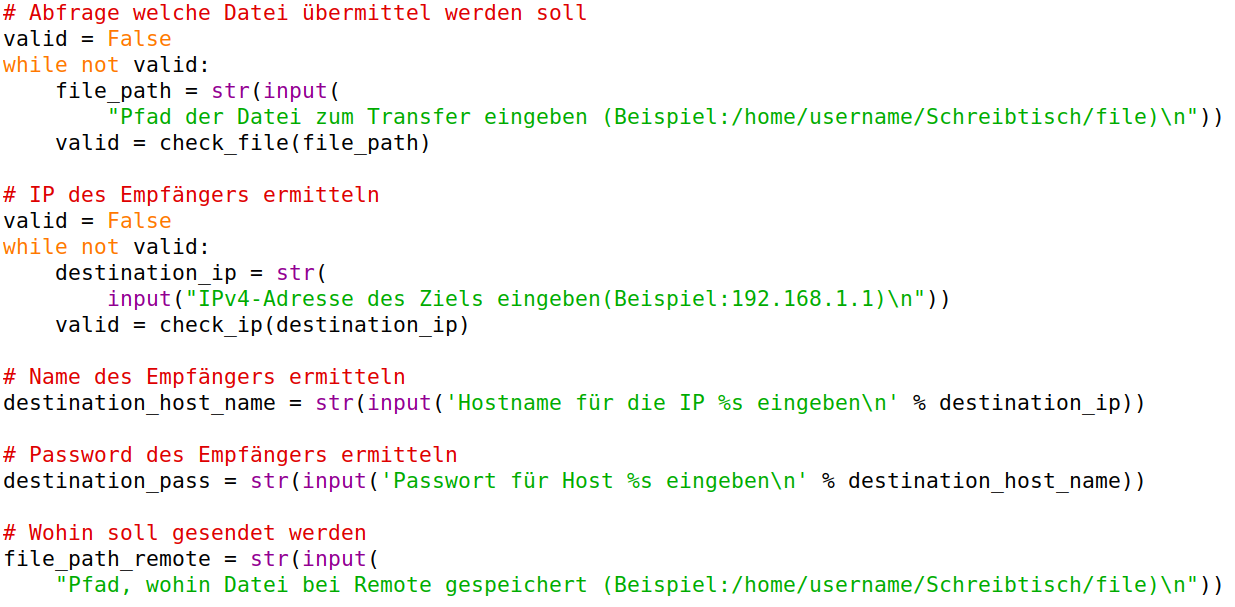
\includegraphics[width=0.8\textwidth]{Bilder/transfer-daten}
 \captionsetup{justification=centering}
 \caption{Abfrage der Daten für den Dateitransfer}
 \label{transfer-daten}
\end{figure}

\begin{figure}[H]
 \centering
 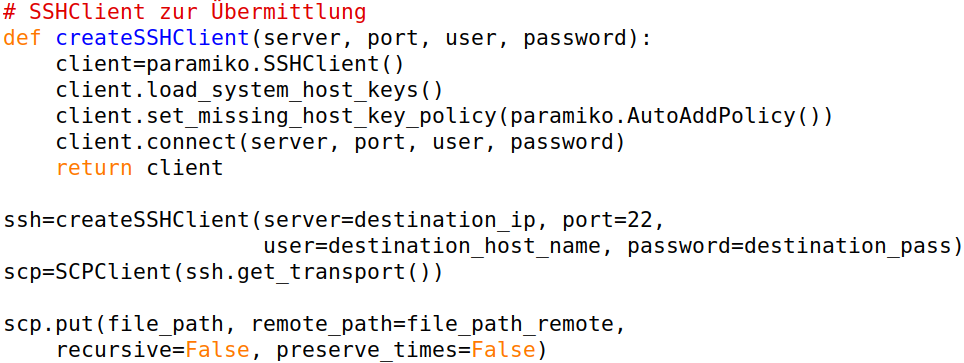
\includegraphics[width=0.8\textwidth]{Bilder/ssh}
 \captionsetup{justification=centering}
 \caption{Übermittlung der Datei über SSH}
 \label{ssh}
\end{figure}

\subsection{Ergebnis}
{\tiny Verfasst von: Mücahit\par}
Über das Python-Skript ist es nun möglich eine Datei priorisiert auf einen Server an der Zentrale zu senden. Das Skript enthält einige Überprüfungen, um beispielsweise zu schauen, ob die eingegebene IP-Adresse und der Dateipfad gültig sind.


\section{Analyse weiterer Netzwerkfunktionen}

\subsection{Hub}
{\tiny Verfasst von: Naghmeh\par}
Repeater arbeiten auf der Ebene 1 des OSI-Modells. Seine Aufgabe ist es, das Signal über dasselbe Netz zu regenerieren, bevor es zu schwach oder beschädigt wird, um die Länge von Signalübertragung im selben Netzwerk zu verlängern. Ein Hub ist im Grunde ein Multiport-Repeater. Ein Hub verbindet mehrere Geräte in einem Netzwerk. Hubs können keine Daten filtern, daher werden Pakete an alle verbundenen Geräte gesendet. Darüber hinaus verfügen sie nicht über die Intelligenz, um den besten Pfad für Pakete zu finden, was zu Ineffizienz und Verschwendung führt.\par
Beim Layer-1-Switching geht es im Wesentlichen um unintelligente Geräte wie Hubs und Repeater. SDN-Switches können so angepasst werden, dass sie sich wie Hubs oder Repeater verhalten. Da Hubs und Repeater keine Informationen speichern können, können Controller bei der Layer-1-Switching keine Datenflüsse weiterleiten. In diesem Fall, jedes Mal, wenn ein Paket ankommt, wird es an den Controller weitergeleitet, der dann entscheidet, alle mit ihm verbundenen Hosts zu überfluten. Dies braucht Zeit, um herauszufinden, wohin das Paket gehen soll, was die Gesamtleistung des Netzes beeinträchtigt.

\subsection{Bridge}
{\tiny Verfasst von: Naghmeh\par}

\subsection{Layer-2-Switch}
{\tiny Verfasst von: Naghmeh\par}

\subsection{Layer-3-Switch}
{\tiny Verfasst von: James\par}
Da Switching schneller als Routing ist, werden in LANS fast nur mit Switches gearbeitet und an zentralen Stellen Router genutzt, um das Internet zu erreichen. Im Netzwerkplan wurde an jeder Lokation nur ein Switch benötigt, dieser musste nicht VLAN fähig sein. Ein Layer-3-Switch ist beispielsweise ein VLAN-fähiger Switch, der grundlegende Routingfunktionalität bietet und auf Ebene 3 des OSI-Modells arbeitet, die Vermittlungsschicht. Das heißt, ein Layer-3-Switch arbeitet mit IP-Adressen und hat mit der Vermittlung von Paketen zu tun. Innerhalb unseres Projekts entschied man sich keine Layer-3-Switches zu nutzen, da die Funktionalitäten des Layer-2-Switches ausgereicht haben. 
\subsection{Dynamic Host Configuration Protocol}
{\tiny Verfasst von: James\par}
DHCP ist ein Dienst, der an das Netzwerk angeschlossene Geräte mit einer Netzwerkkonfiguration versorgt. Falls ein Gerät eine Konfiguration benötigt, wird dies mithilfe vom DHCP Server konfiguriert, dieser kann beispielsweise im Router des Netzwerks sein. Mithilfe von Mininet konnte eine DHCP Konfiguration realisiert werden. Bis zu diesem Punkt wurde die IP-Adressverwaltung ohne DHCP realisiert. Das heißt, jeder Host musste manuell eine IP-Adresse zugewiesen bekommen. Diese manuelle Konfiguration wurde durch eine for-Schleife im Skript (siehe Abbildung \ref{fororig}) durchgeführt.

\begin{figure}[H]
 \centering
 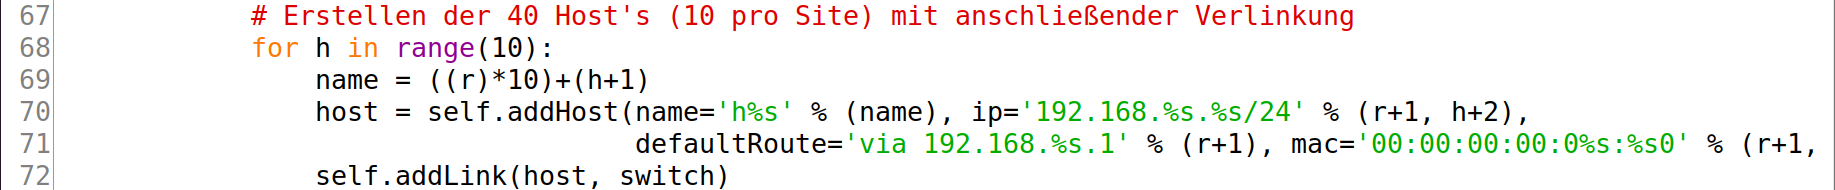
\includegraphics[width=0.8\textwidth]{Bilder/fororig}
 \captionsetup{justification=centering}
 \caption{Statische IP-Adressenverwaltung}
 \label{fororig}
\end{figure}

Bei aktivierten DHCP in Mininet verwaltet der DHCP-Server IP-Adressen ohne manuellen Eingriff des Administrators und weist jedem Host eine IP-Adresse zu. Somit wurde die Funktion der for-Schleife umgeändert, sodass jeder Host von Beginn an die IP-Adresse \textit{\textbf{0.0.0.0}} zugewiesen bekommt. Dadurch wird dem Host keine IP-Adresse manuell zugeteilt. Die IP-Adressverwaltung wird vom DHCP-Server übernommen (siehe Abbildung \ref{forneu}).
  
\begin{figure}[H]
 \centering
 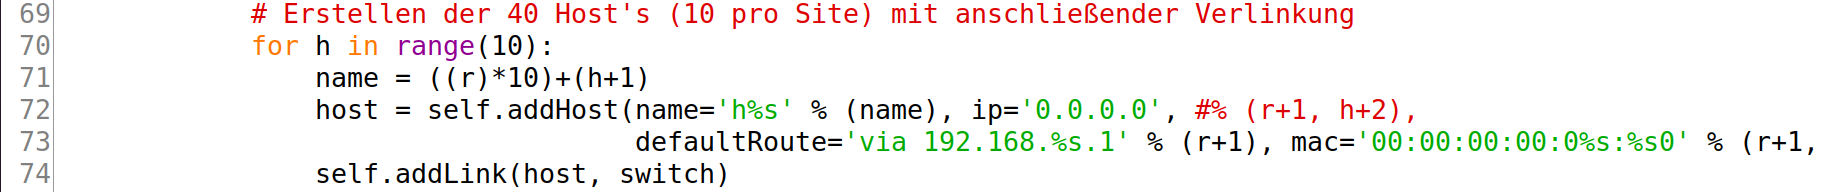
\includegraphics[width=0.8\textwidth]{Bilder/forneu}
 \captionsetup{justification=centering}
 \caption{Dynamische IP-Adressenverwaltung}
 \label{forneu}
\end{figure}

\subsubsection{Durchführung}
{\tiny Verfasst von: James\par}
\begin{wrapfigure}{r}{0.5\textwidth}
	\vspace{-\baselineskip}
 	\centering
 	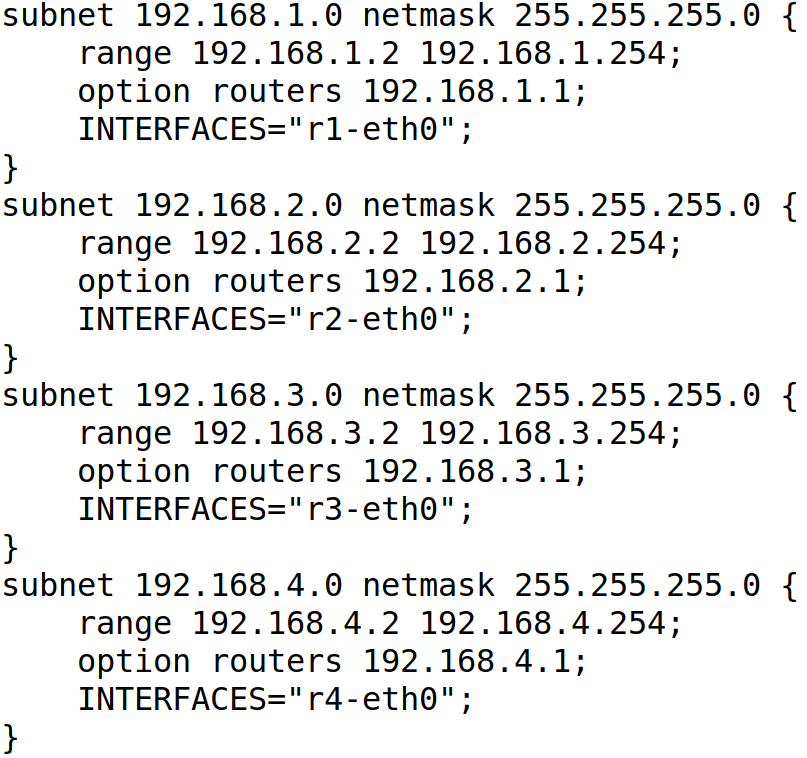
\includegraphics[width=0.4\textwidth]{Bilder/dhcp2}
 	\caption{DHCP-Konfiguration für alle Standorte}
 	\label{dhcp2}
\end{wrapfigure}
Um ein DHCP Server im Netzwerk zu realisieren, muss als erstes der DHCP server auf die VM installiert werden. Dies wird mit dem Befehl \textit{\textbf{sudo apt-get install isc.dhcp-server}} durchgeführt. Als zweites muss im Mininet-Skript die Zeile \textit{\textbf{os.system(“service isc-dhcp-server restart”)}} ergänzt werden, um den DHCP-Server neu zu starten. Anschließend wird der DHCP server konfiguriert. Dies erfolgt in der \textit{\textbf{dhcpd.conf}} Datei, die sich im Pfad \textit{\textbf{/etc/dhcp}} befindet (siehe Abbildung \ref{dhcp2}). In dieser Datei werden die von den DHCP-Clients benötigten Netzwerkkonfigurationsinformationen gespeichert. Da das Netzwerk aus vier Subnetzen besteht, die mit dem DHCP-Server verbunden sein sollen, müssen vier Subnetze in der \textit{\textbf{dhcpd.conf}} Datei definiert werden. Diese Subnetze benötigen folgende Parameter: \textit{\textbf{subnet, netmask, range, option routers, default-lease-time, max-lease-time}} und \textit{\textbf{INTERFACES}}. Wie in der Tabelle des Netzwerkplans vorgezeigt (siehe Abbildung \ref{netzwerkplan}), hat jede Lokation eine festgelegte Subnetz IP (\textit{\textbf{subnet}}), Netzwerkmaske (\textit{\textbf{netmask}}) und Router IP (\textit{\textbf{option routers}}) und wird hier definiert. Um allen Hosts in den jeweiligen Subnetzen dynamisch Adressen zuzuweisen, muss innerhalb der Subnetz-Deklaration ein Bereich definiert werden (\textit{\textbf{range}}). Anschließend wird definiert, an welches Netzwerkgerät der DHCP-Server verbunden werden soll (\textit{\textbf{INTERFACES}}). Es kann auch die Gültigkeitsdauer definiert werden, die angibt wie lange einem Host die IP-Adresse zu Verfügung steht. Normalerweise reichen die Voreinstellungen aus, können aber mit \textit{\textbf{default-lease-time}} und \textit{\textbf{max-lease-time}} erhöhen oder herabsetzen, je nach Notwendigkeit. Anhand dieser Informationen, kann für jeden Standort ein Subnetz definiert werden. 

\subsubsection{Ergebnis}
{\tiny Verfasst von: James\par}
Nachdem das Mininet Skript ausgeführt wird, kann mit Wireshark geprüft werden, ob ein DHCP-Server richtig implementiert wurde. Aus der folgenden Abbildung \ref{wireshark} ist ersichtlich, dass die Pakete zwischen h1 (192.168.1.2) und h11 (192.168.2.2) übertragen werden.
\begin{figure}[H]
 \centering
 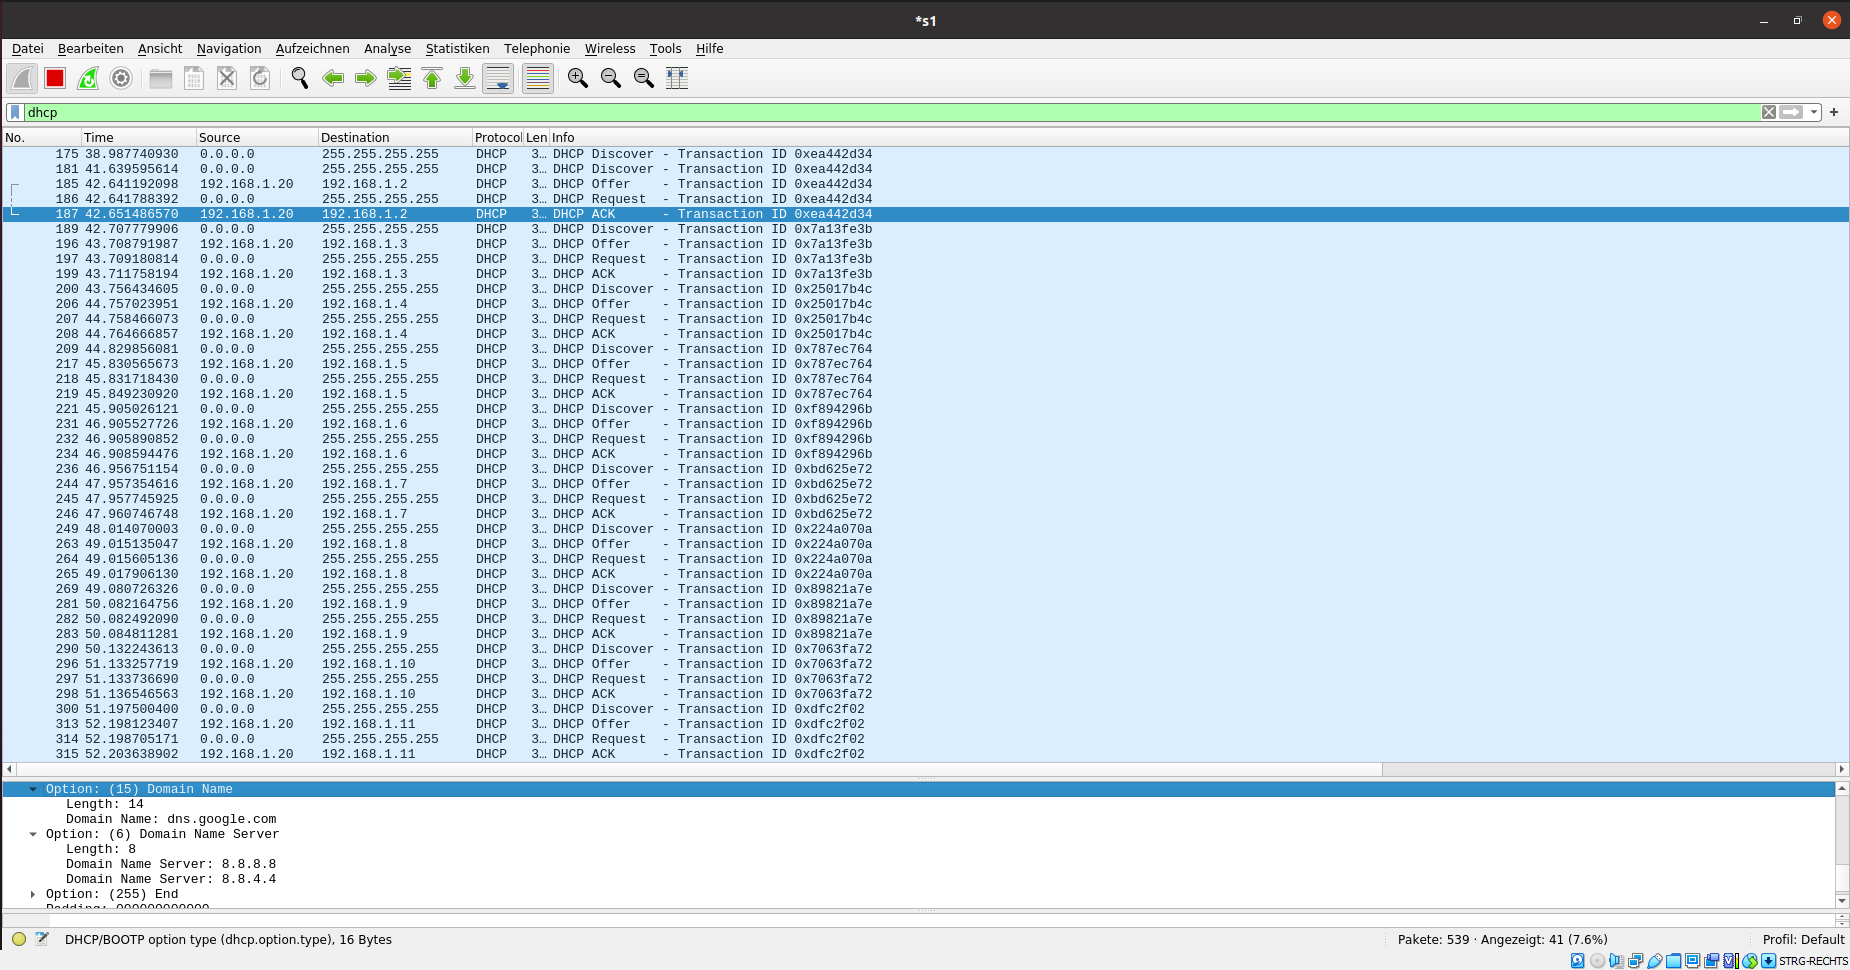
\includegraphics[width=1.0\textwidth]{Bilder/wireshark}
 \captionsetup{justification=centering}
 \caption{Datenverkehr zwischen h1 und h11}
 \label{wireshark}
\end{figure}

Um die Netzwerkkonfiguration vom DHCP-Server zu betrachten, muss Wireshark vor Mininet gestartet und beim Ausführen des Mininet Skripts eine Switch betrachtet werden. In diesem Beispiel wird die Lokation Frankfurt betrachtet (siehe Abbildung \ref{s1}).

\begin{figure}[H]
 \centering
 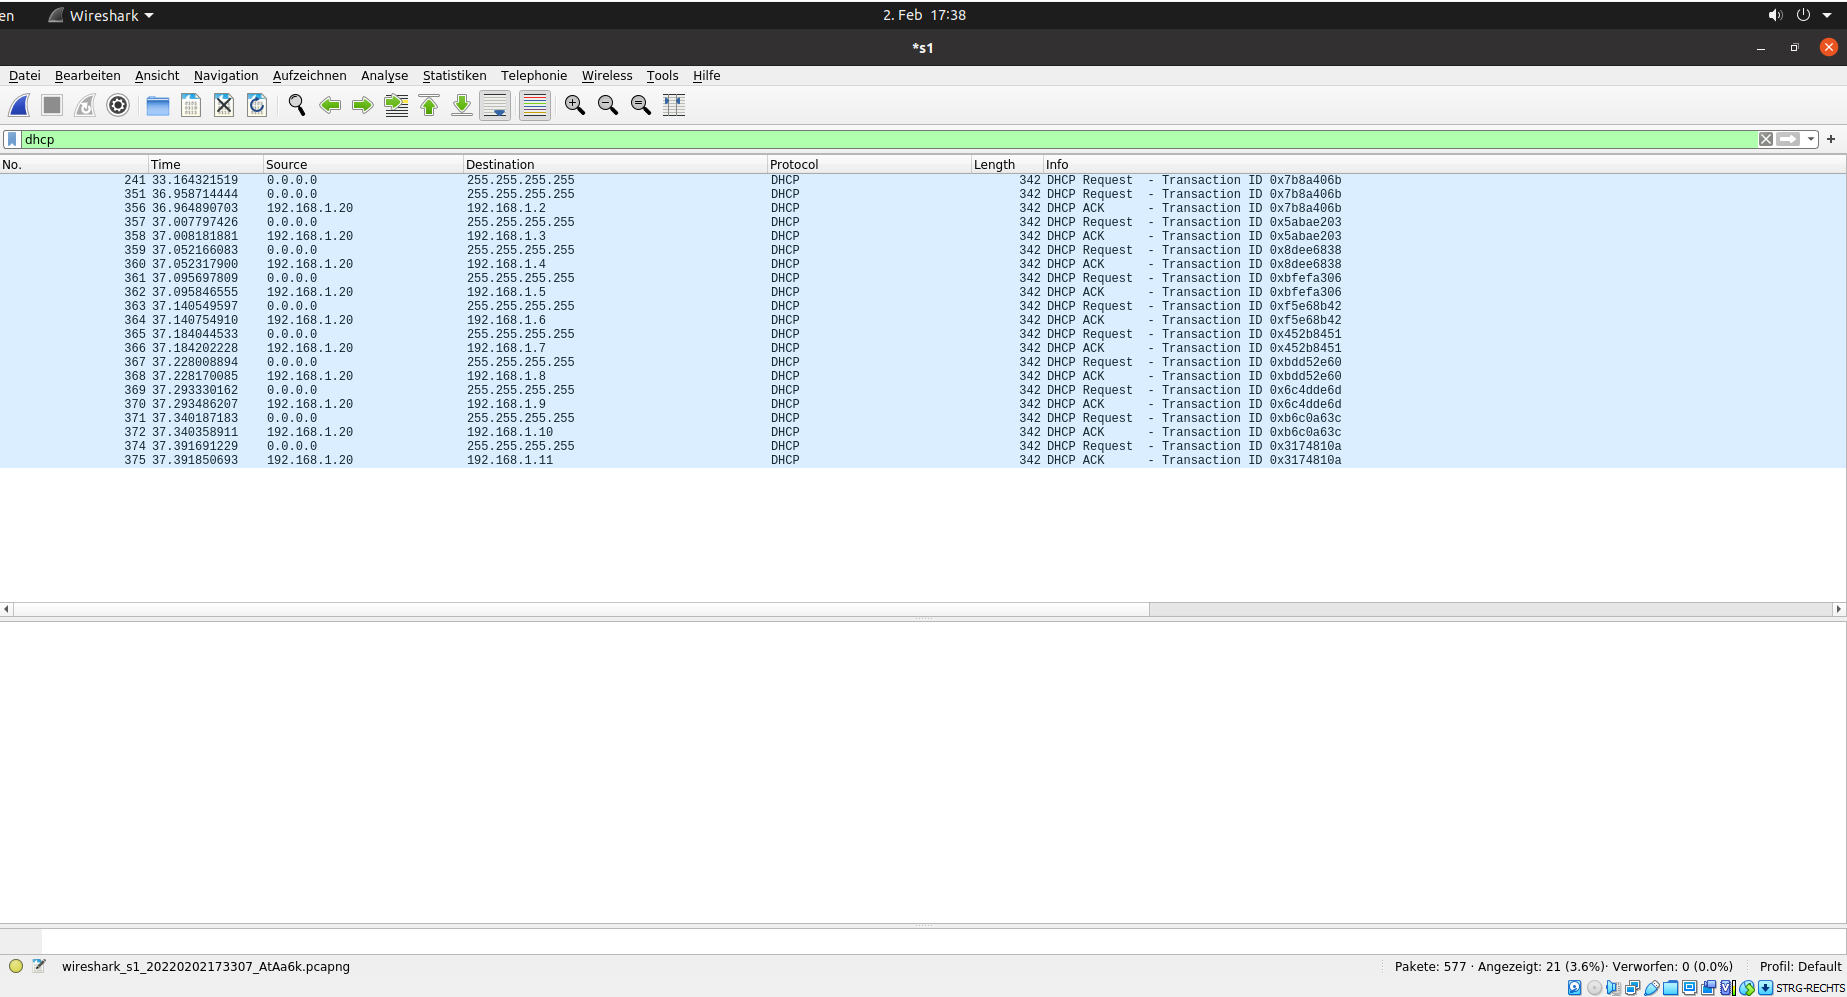
\includegraphics[width=1.0\textwidth]{Bilder/s1}
 \captionsetup{justification=centering}
 \caption{Wireshark-Aufnahme der Switch s1 (Frankfurt)}
 \label{s1}
\end{figure}


\subsection{Domain Name System}
{\tiny Verfasst von: James\par}


\chapter{Diskussion der Ergebnisse}
{\tiny Verfasst von: ?, ?, ?, ?\par}
Analyse der Ergebnisse
Kritische Betrachtung
Hier erwähnen welche Teile der Aufgaben nicht geklappt haben, wie beispielsweise Aufgabe 5 Webproxy
\section{Analyse der Ergebnisse}
{\tiny Verfasst von: ?, ?, ?, ?\par}
\section{Kritische Betrachtung}
{\tiny Verfasst von: ?, ?, ?, ?\par}

\chapter{Fazit}\label{ch:fazit}
{\tiny Verfasst von: ?, ?, ?, ?\par}
Eventuell als Überpunkt zu Gesamtergebnis?
Was ist der finale Stand des Projekts?
Inwiefern wurden die Ziele erreicht?

1. Fragestellung/Aufgabenstellung kurz einführen wieder
2. Zusammenfassen
3. Wurden die Ziele erreicht
scribbr.de
\section{Zukunftsaussichten}
{\tiny Verfasst von: ?, ?, ?, ?\par}
Inwiefern können die Ergebnisse des Projekts weiter genutzt werden?
\par


\printbibliography[title=Literaturverzeichnis]

\end{document}